\documentclass[a4paper]{book}
\usepackage{makeidx}
\usepackage{graphicx}
\usepackage{multicol}
\usepackage{float}
\usepackage{listings}
\usepackage{color}
\usepackage{ifthen}
\usepackage[table]{xcolor}
\usepackage{textcomp}
\usepackage{alltt}
\usepackage{ifpdf}
\ifpdf
\usepackage[pdftex,
            pagebackref=true,
            colorlinks=true,
            linkcolor=blue,
            unicode
           ]{hyperref}
\else
\usepackage[ps2pdf,
            pagebackref=true,
            colorlinks=true,
            linkcolor=blue,
            unicode
           ]{hyperref}
\usepackage{pspicture}
\fi
\usepackage[utf8]{inputenc}
\usepackage{mathptmx}
\usepackage[scaled=.90]{helvet}
\usepackage{courier}
\usepackage{sectsty}
\usepackage[titles]{tocloft}
\usepackage{doxygen}
\lstset{language=C++,inputencoding=utf8,basicstyle=\footnotesize,breaklines=true,breakatwhitespace=true,tabsize=2,numbers=left }
\makeindex
\setcounter{tocdepth}{3}
\renewcommand{\footrulewidth}{0.4pt}
\renewcommand{\familydefault}{\sfdefault}
\begin{document}
\hypersetup{pageanchor=false}
\begin{titlepage}
\vspace*{7cm}
\begin{center}
{\Large ecosistem\_\-1.0 \\[1ex]\large 1.0 }\\
\vspace*{1cm}
{\large Generated by Doxygen 1.7.4}\\
\vspace*{0.5cm}
{\small Wed Feb 29 2012 13:15:13}\\
\end{center}
\end{titlepage}
\clearemptydoublepage
\pagenumbering{roman}
\tableofcontents
\clearemptydoublepage
\pagenumbering{arabic}
\hypersetup{pageanchor=true}
\chapter{Ecosystem Simulator}
\label{index}\hypertarget{index}{}\hypertarget{index_intro}{}\section{Introduction}\label{index_intro}
this project is a didactic project which aim is to model and simulate the evolution of an ecosystem.\hypertarget{index_features}{}\section{Model Features}\label{index_features}
the ecosystem is developed to have the following features:\hypertarget{index_n_species}{}\subsection{N Species}\label{index_n_species}
the ecosystem could have n species whith different parameters\hypertarget{index_mutual_appetite}{}\subsection{Mutual Appetite}\label{index_mutual_appetite}
each species could like, and so eat, each other. selected a species the user can set how much a species like another. rabbit like carrot but doesn't like wolf.\hypertarget{index_gender}{}\subsection{Vivent Gender}\label{index_gender}
vivent could have a gender: male, female, asexual, ermaphrodite. in this realize animals could only be male or female. no vegetable reproduction is modeled nor implemented so vegetable gender is only asexual;\hypertarget{index_purposes}{}\section{Purposes}\label{index_purposes}
as already said this project has only didactic purposes. i can't really assure that it can produce good result from a scientific point of view. my real purpose was to develop something that could be expanded easily in future realizes, and of course have practice whith OO programming and boost features like multi index containers which are the key components of this project.\hypertarget{index_vivent_model}{}\section{Vivent Model}\label{index_vivent_model}
vivent are modelized giving them differents parameters. you can see them by looking to the vivent's inheritance tree. 
\chapter{Todo List}
\label{todo}
\hypertarget{todo}{}
\label{todo__todo000001}
\hypertarget{todo__todo000001}{}
 
\begin{DoxyDescription}
\item[Member \hyperlink{classEcosystemContainer_ac2c4ace58f9adbb265f61057420c5565}{EcosystemContainer::is\_\-full}() ]implement 
\end{DoxyDescription}

\label{todo__todo000003}
\hypertarget{todo__todo000003}{}
 
\begin{DoxyDescription}
\item[Member \hyperlink{classEcosystemContainer_a236c01266343664efab29b1a73e72d1d}{EcosystemContainer::step}(\hyperlink{structStepLog}{StepLog} \&log) ]could be a good idea to make the whole couple migrate 
\end{DoxyDescription}

\label{todo__todo000002}
\hypertarget{todo__todo000002}{}
 
\begin{DoxyDescription}
\item[Member \hyperlink{structSpeciesInfo_a109b3e5acaf126bb8df9648b6c925542}{SpeciesInfo::likings} ]scrivi delle considerazioni finali sul fatto che i multi\_\-index sono più comodi in questi casi anche per emulare una map isi isi 
\end{DoxyDescription}
\chapter{Class Index}
\section{Class Hierarchy}
This inheritance list is sorted roughly, but not completely, alphabetically:\begin{DoxyCompactList}
\item \contentsline{section}{AbstractClock}{\pageref{classAbstractClock}}{}
\begin{DoxyCompactList}
\item \contentsline{section}{Clock}{\pageref{classClock}}{}
\end{DoxyCompactList}
\item \contentsline{section}{change\_\-animal\_\-appetite}{\pageref{structchange__animal__appetite}}{}
\item \contentsline{section}{change\_\-animal\_\-hp}{\pageref{structchange__animal__hp}}{}
\item \contentsline{section}{change\_\-animal\_\-libido}{\pageref{structchange__animal__libido}}{}
\item \contentsline{section}{eco::Container}{\pageref{classeco_1_1Container}}{}
\begin{DoxyCompactList}
\item \contentsline{section}{EcosystemContainer}{\pageref{classEcosystemContainer}}{}
\item \contentsline{section}{Like}{\pageref{structLike}}{}
\item \contentsline{section}{SpeciesInfo}{\pageref{structSpeciesInfo}}{}
\item \contentsline{section}{SubsystemContainer}{\pageref{classSubsystemContainer}}{}
\end{DoxyCompactList}
\item \contentsline{section}{Controller}{\pageref{classController}}{}
\begin{DoxyCompactList}
\item \contentsline{section}{SpeciesController}{\pageref{classSpeciesController}}{}
\end{DoxyCompactList}
\item \contentsline{section}{DateOfBirth}{\pageref{classDateOfBirth}}{}
\item \contentsline{section}{SubsystemContainer::eat}{\pageref{structSubsystemContainer_1_1eat}}{}
\item \contentsline{section}{Existance}{\pageref{classExistance}}{}
\begin{DoxyCompactList}
\item \contentsline{section}{Vivent}{\pageref{classVivent}}{}
\begin{DoxyCompactList}
\item \contentsline{section}{Specied}{\pageref{classSpecied}}{}
\begin{DoxyCompactList}
\item \contentsline{section}{Animal}{\pageref{classAnimal}}{}
\begin{DoxyCompactList}
\item \contentsline{section}{IndividualAnimal}{\pageref{classIndividualAnimal}}{}
\end{DoxyCompactList}
\item \contentsline{section}{Vegetable}{\pageref{classVegetable}}{}
\begin{DoxyCompactList}
\item \contentsline{section}{IndividualVegetable}{\pageref{classIndividualVegetable}}{}
\end{DoxyCompactList}
\end{DoxyCompactList}
\end{DoxyCompactList}
\end{DoxyCompactList}
\item \contentsline{section}{Gender}{\pageref{classGender}}{}
\item \contentsline{section}{Grafico}{\pageref{classGrafico}}{}
\item \contentsline{section}{SubsystemContainer::id}{\pageref{structSubsystemContainer_1_1id}}{}
\item \contentsline{section}{LikeFactorCmp}{\pageref{structLikeFactorCmp}}{}
\item \contentsline{section}{LikeRefCmp}{\pageref{structLikeRefCmp}}{}
\item \contentsline{section}{PopulationVariation}{\pageref{structPopulationVariation}}{}
\item \contentsline{section}{SubsystemContainer::reproduction}{\pageref{structSubsystemContainer_1_1reproduction}}{}
\item \contentsline{section}{SubsystemContainer::spec\_\-id}{\pageref{structSubsystemContainer_1_1spec__id}}{}
\item \contentsline{section}{StepLog}{\pageref{structStepLog}}{}
\end{DoxyCompactList}

\chapter{Class Index}
\section{Class List}
Here are the classes, structs, unions and interfaces with brief descriptions:\begin{DoxyCompactList}
\item\contentsline{section}{\hyperlink{classAbstractClock}{AbstractClock} (Abstract class for the clock )}{\pageref{classAbstractClock}}{}
\item\contentsline{section}{\hyperlink{classAnimal}{Animal} (Class \hyperlink{classAnimal}{Animal} )}{\pageref{classAnimal}}{}
\item\contentsline{section}{\hyperlink{structchange__animal__appetite}{change\_\-animal\_\-appetite} (Functor to change \hyperlink{classIndividualAnimal}{IndividualAnimal} appetite )}{\pageref{structchange__animal__appetite}}{}
\item\contentsline{section}{\hyperlink{structchange__animal__hp}{change\_\-animal\_\-hp} (Functor to change \hyperlink{classIndividualAnimal}{IndividualAnimal} hp )}{\pageref{structchange__animal__hp}}{}
\item\contentsline{section}{\hyperlink{structchange__animal__libido}{change\_\-animal\_\-libido} (Functor to cahnge \hyperlink{classIndividualAnimal}{IndividualAnimal} libido )}{\pageref{structchange__animal__libido}}{}
\item\contentsline{section}{\hyperlink{classClock}{Clock} (Real clock able to give the time of the sistem )}{\pageref{classClock}}{}
\item\contentsline{section}{\hyperlink{classeco_1_1Container}{eco::Container} (\hyperlink{classeco_1_1Container}{Container} abstract class )}{\pageref{classeco_1_1Container}}{}
\item\contentsline{section}{\hyperlink{classController}{Controller} (Class that generally controll )}{\pageref{classController}}{}
\item\contentsline{section}{\hyperlink{classDateOfBirth}{DateOfBirth} (Simple class for the date of birh )}{\pageref{classDateOfBirth}}{}
\item\contentsline{section}{\hyperlink{structSubsystemContainer_1_1eat}{SubsystemContainer::eat} (Boost multyindex::ordered\_\-index tag )}{\pageref{structSubsystemContainer_1_1eat}}{}
\item\contentsline{section}{\hyperlink{classEcosystemContainer}{EcosystemContainer} (All the form of life )}{\pageref{classEcosystemContainer}}{}
\item\contentsline{section}{\hyperlink{classExistance}{Existance} (Class \hyperlink{classExistance}{Existance} the most abstracted object )}{\pageref{classExistance}}{}
\item\contentsline{section}{\hyperlink{classGender}{Gender} (\hyperlink{classGender}{Gender} of the form of life )}{\pageref{classGender}}{}
\item\contentsline{section}{\hyperlink{classGrafico}{Grafico} }{\pageref{classGrafico}}{}
\item\contentsline{section}{\hyperlink{structSubsystemContainer_1_1id}{SubsystemContainer::id} (Boost multyindex::ordered\_\-index tag )}{\pageref{structSubsystemContainer_1_1id}}{}
\item\contentsline{section}{\hyperlink{classIndividualAnimal}{IndividualAnimal} (Class \hyperlink{classIndividualAnimal}{IndividualAnimal} )}{\pageref{classIndividualAnimal}}{}
\item\contentsline{section}{\hyperlink{classIndividualVegetable}{IndividualVegetable} (Class \hyperlink{classIndividualVegetable}{IndividualVegetable} )}{\pageref{classIndividualVegetable}}{}
\item\contentsline{section}{\hyperlink{structLike}{Like} (How much a species is liked by another )}{\pageref{structLike}}{}
\item\contentsline{section}{\hyperlink{structLikeFactorCmp}{LikeFactorCmp} }{\pageref{structLikeFactorCmp}}{}
\item\contentsline{section}{\hyperlink{structLikeRefCmp}{LikeRefCmp} (Used in SpeciesInfo.h )}{\pageref{structLikeRefCmp}}{}
\item\contentsline{section}{\hyperlink{structPopulationVariation}{PopulationVariation} (Variation of population for a species in a subsystemcontainer )}{\pageref{structPopulationVariation}}{}
\item\contentsline{section}{\hyperlink{structSubsystemContainer_1_1reproduction}{SubsystemContainer::reproduction} (Boost multyindex::ordered\_\-index tag )}{\pageref{structSubsystemContainer_1_1reproduction}}{}
\item\contentsline{section}{\hyperlink{structSubsystemContainer_1_1spec__id}{SubsystemContainer::spec\_\-id} (Boost multyindex::ordered\_\-index tag )}{\pageref{structSubsystemContainer_1_1spec__id}}{}
\item\contentsline{section}{\hyperlink{classSpecied}{Specied} (Class \hyperlink{classSpecied}{Specied} the form of life as species belonger )}{\pageref{classSpecied}}{}
\item\contentsline{section}{\hyperlink{classSpeciesController}{SpeciesController} (Contain info about the species in the ecosystem )}{\pageref{classSpeciesController}}{}
\item\contentsline{section}{\hyperlink{structSpeciesInfo}{SpeciesInfo} (Species info containers )}{\pageref{structSpeciesInfo}}{}
\item\contentsline{section}{\hyperlink{structStepLog}{StepLog} (Log of the function step )}{\pageref{structStepLog}}{}
\item\contentsline{section}{\hyperlink{classSubsystemContainer}{SubsystemContainer} (Sub ecosystem container )}{\pageref{classSubsystemContainer}}{}
\item\contentsline{section}{\hyperlink{classVegetable}{Vegetable} (Class \hyperlink{classVegetable}{Vegetable} )}{\pageref{classVegetable}}{}
\item\contentsline{section}{\hyperlink{classVivent}{Vivent} (Class \hyperlink{classVivent}{Vivent} contain HP )}{\pageref{classVivent}}{}
\end{DoxyCompactList}

\chapter{File Index}
\section{File List}
Here is a list of all documented files with brief descriptions:\begin{DoxyCompactList}
\item\contentsline{section}{sources/\hyperlink{animal_8cpp}{animal.cpp} }{\pageref{animal_8cpp}}{}
\item\contentsline{section}{sources/\hyperlink{animal_8h}{animal.h} }{\pageref{animal_8h}}{}
\item\contentsline{section}{sources/\hyperlink{beeings_8h}{beeings.h} }{\pageref{beeings_8h}}{}
\item\contentsline{section}{sources/\hyperlink{classcompares_8hpp}{classcompares.hpp} }{\pageref{classcompares_8hpp}}{}
\item\contentsline{section}{sources/{\bfseries container.cpp} }{\pageref{container_8cpp}}{}
\item\contentsline{section}{sources/{\bfseries container.h} }{\pageref{container_8h}}{}
\item\contentsline{section}{sources/{\bfseries controller.cpp} }{\pageref{controller_8cpp}}{}
\item\contentsline{section}{sources/\hyperlink{controller_8h}{controller.h} }{\pageref{controller_8h}}{}
\item\contentsline{section}{sources/{\bfseries disegna.cpp} }{\pageref{disegna_8cpp}}{}
\item\contentsline{section}{sources/{\bfseries draw\_\-evolv.cpp} }{\pageref{draw__evolv_8cpp}}{}
\item\contentsline{section}{sources/{\bfseries ecosystem.cpp} }{\pageref{ecosystem_8cpp}}{}
\item\contentsline{section}{sources/\hyperlink{ecosystem_8h}{ecosystem.h} }{\pageref{ecosystem_8h}}{}
\item\contentsline{section}{sources/\hyperlink{existance_8cpp}{existance.cpp} }{\pageref{existance_8cpp}}{}
\item\contentsline{section}{sources/\hyperlink{existance_8h}{existance.h} }{\pageref{existance_8h}}{}
\item\contentsline{section}{sources/\hyperlink{fieldchangers_8hpp}{fieldchangers.hpp} }{\pageref{fieldchangers_8hpp}}{}
\item\contentsline{section}{sources/{\bfseries fill\_\-random\_\-draw.cpp} }{\pageref{fill__random__draw_8cpp}}{}
\item\contentsline{section}{sources/{\bfseries fill\_\-random\_\-result.cpp} }{\pageref{fill__random__result_8cpp}}{}
\item\contentsline{section}{sources/{\bfseries fill\_\-stream\_\-draw.cpp} }{\pageref{fill__stream__draw_8cpp}}{}
\item\contentsline{section}{sources/{\bfseries fill\_\-stream\_\-result.cpp} }{\pageref{fill__stream__result_8cpp}}{}
\item\contentsline{section}{sources/\hyperlink{gender_8cpp}{gender.cpp} }{\pageref{gender_8cpp}}{}
\item\contentsline{section}{sources/\hyperlink{gender_8h}{gender.h} (\hyperlink{classGender}{Gender} class interface )}{\pageref{gender_8h}}{}
\item\contentsline{section}{sources/{\bfseries grafico.cpp} }{\pageref{grafico_8cpp}}{}
\item\contentsline{section}{sources/{\bfseries grafico.hpp} }{\pageref{grafico_8hpp}}{}
\item\contentsline{section}{sources/\hyperlink{individualanimal_8cpp}{individualanimal.cpp} }{\pageref{individualanimal_8cpp}}{}
\item\contentsline{section}{sources/\hyperlink{individualanimal_8h}{individualanimal.h} }{\pageref{individualanimal_8h}}{}
\item\contentsline{section}{sources/{\bfseries individualvegetable.cpp} }{\pageref{individualvegetable_8cpp}}{}
\item\contentsline{section}{sources/\hyperlink{individualvegetable_8h}{individualvegetable.h} }{\pageref{individualvegetable_8h}}{}
\item\contentsline{section}{sources/{\bfseries like.cpp} }{\pageref{like_8cpp}}{}
\item\contentsline{section}{sources/{\bfseries like.h} }{\pageref{like_8h}}{}
\item\contentsline{section}{sources/{\bfseries main.cpp} }{\pageref{main_8cpp}}{}
\item\contentsline{section}{sources/{\bfseries mainpage.cpp} }{\pageref{mainpage_8cpp}}{}
\item\contentsline{section}{sources/\hyperlink{miscellaneus_8h}{miscellaneus.h} (Wrapper containing miscellaneus and varius classes )}{\pageref{miscellaneus_8h}}{}
\item\contentsline{section}{sources/{\bfseries populationvariation.hpp} }{\pageref{populationvariation_8hpp}}{}
\item\contentsline{section}{sources/{\bfseries specied.cpp} }{\pageref{specied_8cpp}}{}
\item\contentsline{section}{sources/\hyperlink{specied_8h}{specied.h} }{\pageref{specied_8h}}{}
\item\contentsline{section}{sources/{\bfseries speciescontroller.cpp} }{\pageref{speciescontroller_8cpp}}{}
\item\contentsline{section}{sources/\hyperlink{speciescontroller_8h}{speciescontroller.h} }{\pageref{speciescontroller_8h}}{}
\item\contentsline{section}{sources/{\bfseries speciesinfo.cpp} }{\pageref{speciesinfo_8cpp}}{}
\item\contentsline{section}{sources/\hyperlink{speciesinfo_8h}{speciesinfo.h} }{\pageref{speciesinfo_8h}}{}
\item\contentsline{section}{sources/{\bfseries step.cpp} }{\pageref{step_8cpp}}{}
\item\contentsline{section}{sources/{\bfseries step\_\-log.cpp} }{\pageref{step__log_8cpp}}{}
\item\contentsline{section}{sources/{\bfseries steplog.hpp} }{\pageref{steplog_8hpp}}{}
\item\contentsline{section}{sources/\hyperlink{subsystemcontainer_8cpp}{subsystemcontainer.cpp} }{\pageref{subsystemcontainer_8cpp}}{}
\item\contentsline{section}{sources/\hyperlink{subsystemcontainer_8h}{subsystemcontainer.h} }{\pageref{subsystemcontainer_8h}}{}
\item\contentsline{section}{sources/{\bfseries test\_\-like\_\-operators.cpp} }{\pageref{test__like__operators_8cpp}}{}
\item\contentsline{section}{sources/{\bfseries time.cpp} }{\pageref{time_8cpp}}{}
\item\contentsline{section}{sources/\hyperlink{time_8h}{time.h} (Classes to manipulate and determine the time of the system )}{\pageref{time_8h}}{}
\item\contentsline{section}{sources/\hyperlink{vegetable_8cpp}{vegetable.cpp} }{\pageref{vegetable_8cpp}}{}
\item\contentsline{section}{sources/\hyperlink{vegetable_8h}{vegetable.h} }{\pageref{vegetable_8h}}{}
\item\contentsline{section}{sources/{\bfseries vivent.cpp} }{\pageref{vivent_8cpp}}{}
\item\contentsline{section}{sources/\hyperlink{vivent_8h}{vivent.h} }{\pageref{vivent_8h}}{}
\end{DoxyCompactList}

\chapter{Class Documentation}
\hypertarget{classAbstractClock}{
\section{AbstractClock Class Reference}
\label{classAbstractClock}\index{AbstractClock@{AbstractClock}}
}


abstract class for the clock  




{\ttfamily \#include $<$time.h$>$}

Inheritance diagram for AbstractClock:\begin{figure}[H]
\begin{center}
\leavevmode
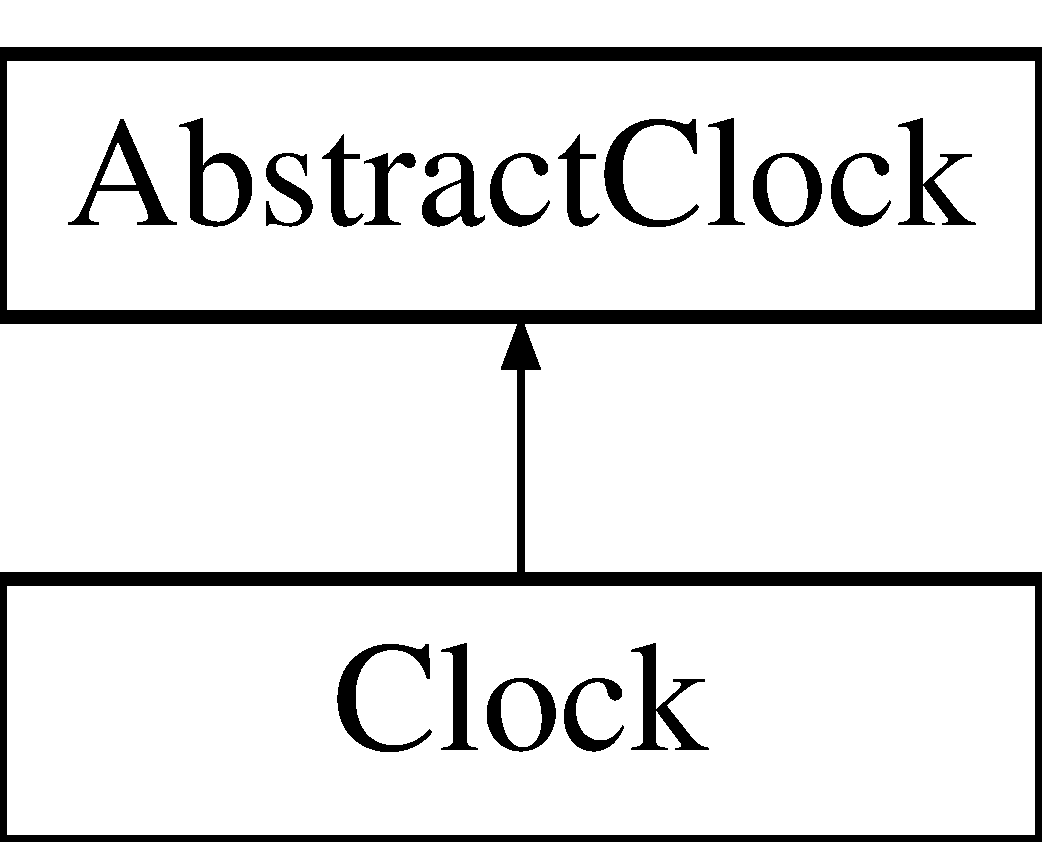
\includegraphics[height=2.000000cm]{classAbstractClock}
\end{center}
\end{figure}
\subsection*{Public Member Functions}
\begin{DoxyCompactItemize}
\item 
virtual void \hyperlink{classAbstractClock_ad161ad323e50eeba01cc97720a2c469e}{tick} (unsigned int times=1)=0
\begin{DoxyCompactList}\small\item\em make the clock tick \end{DoxyCompactList}\end{DoxyCompactItemize}


\subsection{Detailed Description}
abstract class for the clock 

Definition at line 53 of file time.h.



\subsection{Member Function Documentation}
\hypertarget{classAbstractClock_ad161ad323e50eeba01cc97720a2c469e}{
\index{AbstractClock@{AbstractClock}!tick@{tick}}
\index{tick@{tick}!AbstractClock@{AbstractClock}}
\subsubsection[{tick}]{\setlength{\rightskip}{0pt plus 5cm}virtual void AbstractClock::tick (
\begin{DoxyParamCaption}
\item[{unsigned int}]{times = {\ttfamily 1}}
\end{DoxyParamCaption}
)\hspace{0.3cm}{\ttfamily  \mbox{[}pure virtual\mbox{]}}}}
\label{classAbstractClock_ad161ad323e50eeba01cc97720a2c469e}


make the clock tick 

abstract function 

Implemented in \hyperlink{classClock_af0ac46dd780987f2daa69d580e4d5d51}{Clock}.



The documentation for this class was generated from the following files:\begin{DoxyCompactItemize}
\item 
sources/\hyperlink{time_8h}{time.h}\item 
sources/time.cpp\end{DoxyCompactItemize}

\hypertarget{classAnimal}{
\section{Animal Class Reference}
\label{classAnimal}\index{Animal@{Animal}}
}


class \hyperlink{classAnimal}{Animal}  




{\ttfamily \#include $<$animal.h$>$}

Inheritance diagram for Animal:\begin{figure}[H]
\begin{center}
\leavevmode
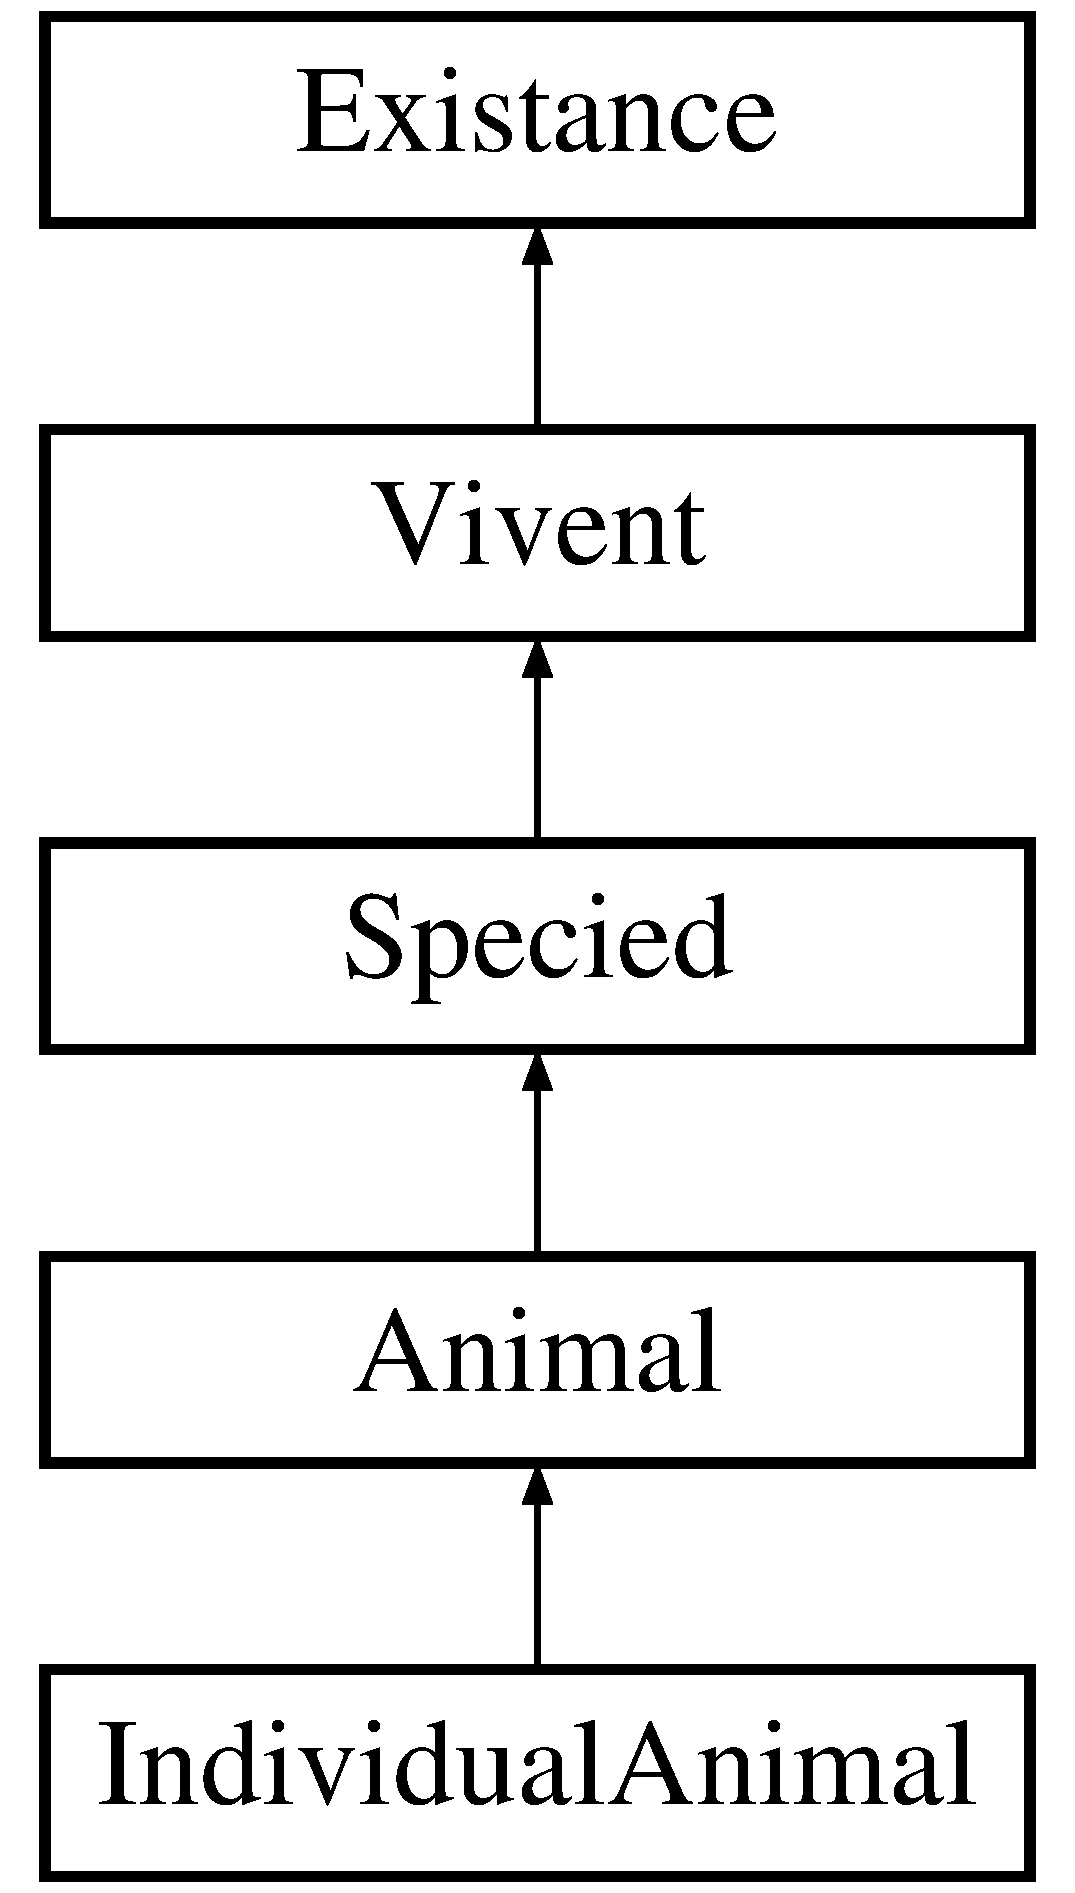
\includegraphics[height=5.000000cm]{classAnimal}
\end{center}
\end{figure}
\subsection*{Public Member Functions}
\begin{DoxyCompactItemize}
\item 
\hyperlink{classAnimal_a4afc6308ef1d106aaed2a5aa61851094}{Animal} (unsigned int u\_\-fight\_\-coast=1)
\begin{DoxyCompactList}\small\item\em default constructor \end{DoxyCompactList}\item 
\hyperlink{classAnimal_a476af25adde5f0dfa688129c8f86fa5c}{$\sim$Animal} ()
\begin{DoxyCompactList}\small\item\em default destructor \end{DoxyCompactList}\item 
virtual void \hyperlink{classAnimal_a4335ec7c755024705ec13084869006f9}{live} ()
\begin{DoxyCompactList}\small\item\em implementation of Specied::live() \end{DoxyCompactList}\item 
\hypertarget{classAnimal_ac18797411b022017013bfcf56e7f9414}{
unsigned int \& \hyperlink{classAnimal_ac18797411b022017013bfcf56e7f9414}{fight\_\-coast} ()}
\label{classAnimal_ac18797411b022017013bfcf56e7f9414}

\begin{DoxyCompactList}\small\item\em set fight coast \end{DoxyCompactList}\item 
\hypertarget{classAnimal_aca7896d9a29f9694dd6c2588fbcc0336}{
unsigned int \hyperlink{classAnimal_aca7896d9a29f9694dd6c2588fbcc0336}{fight\_\-coast} () const }
\label{classAnimal_aca7896d9a29f9694dd6c2588fbcc0336}

\begin{DoxyCompactList}\small\item\em get fight coast \end{DoxyCompactList}\end{DoxyCompactItemize}
\subsection*{Private Attributes}
\begin{DoxyCompactItemize}
\item 
unsigned int \hyperlink{classAnimal_a5f4e339fc2c5c487e9bec9e3bbb2d5ff}{m\_\-fight\_\-coast}
\begin{DoxyCompactList}\small\item\em fight coast is the coast to pay everytime a fight occours \end{DoxyCompactList}\end{DoxyCompactItemize}


\subsection{Detailed Description}
class \hyperlink{classAnimal}{Animal} 

this class rappresents the animal as a form of life able to move and eat. animals can eat other animals or vegetables. it depends from the liking between the species of the two form of lifes 

Definition at line 37 of file animal.h.



\subsection{Constructor \& Destructor Documentation}
\hypertarget{classAnimal_a4afc6308ef1d106aaed2a5aa61851094}{
\index{Animal@{Animal}!Animal@{Animal}}
\index{Animal@{Animal}!Animal@{Animal}}
\subsubsection[{Animal}]{\setlength{\rightskip}{0pt plus 5cm}Animal::Animal (
\begin{DoxyParamCaption}
\item[{unsigned int}]{u\_\-fight\_\-coast = {\ttfamily 1}}
\end{DoxyParamCaption}
)}}
\label{classAnimal_a4afc6308ef1d106aaed2a5aa61851094}


default constructor 

does nothing 

Definition at line 35 of file animal.cpp.

\hypertarget{classAnimal_a476af25adde5f0dfa688129c8f86fa5c}{
\index{Animal@{Animal}!$\sim$Animal@{$\sim$Animal}}
\index{$\sim$Animal@{$\sim$Animal}!Animal@{Animal}}
\subsubsection[{$\sim$Animal}]{\setlength{\rightskip}{0pt plus 5cm}Animal::$\sim$Animal (
\begin{DoxyParamCaption}
{}
\end{DoxyParamCaption}
)}}
\label{classAnimal_a476af25adde5f0dfa688129c8f86fa5c}


default destructor 

does nothing 

Definition at line 40 of file animal.cpp.



\subsection{Member Function Documentation}
\hypertarget{classAnimal_a4335ec7c755024705ec13084869006f9}{
\index{Animal@{Animal}!live@{live}}
\index{live@{live}!Animal@{Animal}}
\subsubsection[{live}]{\setlength{\rightskip}{0pt plus 5cm}void Animal::live (
\begin{DoxyParamCaption}
{}
\end{DoxyParamCaption}
)\hspace{0.3cm}{\ttfamily  \mbox{[}virtual\mbox{]}}}}
\label{classAnimal_a4335ec7c755024705ec13084869006f9}


implementation of Specied::live() 

\begin{DoxySeeAlso}{See also}
Specied::live() 
\end{DoxySeeAlso}


Definition at line 45 of file animal.cpp.



\subsection{Member Data Documentation}
\hypertarget{classAnimal_a5f4e339fc2c5c487e9bec9e3bbb2d5ff}{
\index{Animal@{Animal}!m\_\-fight\_\-coast@{m\_\-fight\_\-coast}}
\index{m\_\-fight\_\-coast@{m\_\-fight\_\-coast}!Animal@{Animal}}
\subsubsection[{m\_\-fight\_\-coast}]{\setlength{\rightskip}{0pt plus 5cm}unsigned int {\bf Animal::m\_\-fight\_\-coast}\hspace{0.3cm}{\ttfamily  \mbox{[}private\mbox{]}}}}
\label{classAnimal_a5f4e339fc2c5c487e9bec9e3bbb2d5ff}


fight coast is the coast to pay everytime a fight occours 

the pay coast is suctract from the hp both of the prey and the predator. 

Definition at line 68 of file animal.h.



The documentation for this class was generated from the following files:\begin{DoxyCompactItemize}
\item 
sources/\hyperlink{animal_8h}{animal.h}\item 
sources/\hyperlink{animal_8cpp}{animal.cpp}\end{DoxyCompactItemize}

\hypertarget{structchange__animal__appetite}{
\section{change\_\-animal\_\-appetite Struct Reference}
\label{structchange__animal__appetite}\index{change\_\-animal\_\-appetite@{change\_\-animal\_\-appetite}}
}


functor to change \hyperlink{classIndividualAnimal}{IndividualAnimal} appetite  




{\ttfamily \#include $<$fieldchangers.hpp$>$}

\subsection*{Public Member Functions}
\begin{DoxyCompactItemize}
\item 
\hypertarget{structchange__animal__appetite_ac41f6ae44d1d5c3326193b242b496270}{
\hyperlink{structchange__animal__appetite_ac41f6ae44d1d5c3326193b242b496270}{change\_\-animal\_\-appetite} (unsigned int nw\_\-appetite)}
\label{structchange__animal__appetite_ac41f6ae44d1d5c3326193b242b496270}

\begin{DoxyCompactList}\small\item\em constructor setting new appetite value \end{DoxyCompactList}\item 
\hypertarget{structchange__animal__appetite_adf55d69d445073e692f68bc06cb3abcf}{
void \hyperlink{structchange__animal__appetite_adf55d69d445073e692f68bc06cb3abcf}{operator()} (\hyperlink{classIndividualAnimal}{IndividualAnimal} \&an)}
\label{structchange__animal__appetite_adf55d69d445073e692f68bc06cb3abcf}

\begin{DoxyCompactList}\small\item\em change the value \end{DoxyCompactList}\end{DoxyCompactItemize}
\subsection*{Private Attributes}
\begin{DoxyCompactItemize}
\item 
\hypertarget{structchange__animal__appetite_a88b4e8d511e5ad5c389e79d7cd47cd7a}{
unsigned int \hyperlink{structchange__animal__appetite_a88b4e8d511e5ad5c389e79d7cd47cd7a}{m\_\-nw\_\-appetite}}
\label{structchange__animal__appetite_a88b4e8d511e5ad5c389e79d7cd47cd7a}

\begin{DoxyCompactList}\small\item\em new appetite value \end{DoxyCompactList}\end{DoxyCompactItemize}


\subsection{Detailed Description}
functor to change \hyperlink{classIndividualAnimal}{IndividualAnimal} appetite 

Definition at line 134 of file fieldchangers.hpp.



The documentation for this struct was generated from the following file:\begin{DoxyCompactItemize}
\item 
sources/\hyperlink{fieldchangers_8hpp}{fieldchangers.hpp}\end{DoxyCompactItemize}

\hypertarget{structchange__animal__hp}{
\section{change\_\-animal\_\-hp Struct Reference}
\label{structchange__animal__hp}\index{change\_\-animal\_\-hp@{change\_\-animal\_\-hp}}
}


functor to change \hyperlink{classIndividualAnimal}{IndividualAnimal} hp  




{\ttfamily \#include $<$fieldchangers.hpp$>$}

\subsection*{Public Member Functions}
\begin{DoxyCompactItemize}
\item 
\hypertarget{structchange__animal__hp_a62c8ac720a8a79c9b07d2b360df7be2d}{
\hyperlink{structchange__animal__hp_a62c8ac720a8a79c9b07d2b360df7be2d}{change\_\-animal\_\-hp} (int \&nw\_\-hp)}
\label{structchange__animal__hp_a62c8ac720a8a79c9b07d2b360df7be2d}

\begin{DoxyCompactList}\small\item\em constructor setting new hp value \end{DoxyCompactList}\item 
\hypertarget{structchange__animal__hp_a1ee9b6cc693ae673b687e7b81e1cdc83}{
void \hyperlink{structchange__animal__hp_a1ee9b6cc693ae673b687e7b81e1cdc83}{operator()} (\hyperlink{classIndividualAnimal}{IndividualAnimal} \&an)}
\label{structchange__animal__hp_a1ee9b6cc693ae673b687e7b81e1cdc83}

\begin{DoxyCompactList}\small\item\em change the value \end{DoxyCompactList}\end{DoxyCompactItemize}
\subsection*{Private Attributes}
\begin{DoxyCompactItemize}
\item 
\hypertarget{structchange__animal__hp_a1a7e86389e8afd8624fdb0a49aabd42c}{
int \hyperlink{structchange__animal__hp_a1a7e86389e8afd8624fdb0a49aabd42c}{m\_\-nw\_\-hp}}
\label{structchange__animal__hp_a1a7e86389e8afd8624fdb0a49aabd42c}

\begin{DoxyCompactList}\small\item\em new hp value \end{DoxyCompactList}\end{DoxyCompactItemize}


\subsection{Detailed Description}
functor to change \hyperlink{classIndividualAnimal}{IndividualAnimal} hp 

this version controll if the hp passed are negative. if so set it to 0 if they'r more than 100 set it to 0 because of uncorrect usage of unsigned int 

Definition at line 68 of file fieldchangers.hpp.



The documentation for this struct was generated from the following file:\begin{DoxyCompactItemize}
\item 
sources/\hyperlink{fieldchangers_8hpp}{fieldchangers.hpp}\end{DoxyCompactItemize}

\hypertarget{structchange__animal__libido}{
\section{change\_\-animal\_\-libido Struct Reference}
\label{structchange__animal__libido}\index{change\_\-animal\_\-libido@{change\_\-animal\_\-libido}}
}


functor to cahnge \hyperlink{classIndividualAnimal}{IndividualAnimal} libido  




{\ttfamily \#include $<$fieldchangers.hpp$>$}

\subsection*{Public Member Functions}
\begin{DoxyCompactItemize}
\item 
\hypertarget{structchange__animal__libido_a5896ac98df3c0d22bf73b154dbdf57e0}{
\hyperlink{structchange__animal__libido_a5896ac98df3c0d22bf73b154dbdf57e0}{change\_\-animal\_\-libido} (unsigned int nw\_\-libido)}
\label{structchange__animal__libido_a5896ac98df3c0d22bf73b154dbdf57e0}

\begin{DoxyCompactList}\small\item\em constructor setting new lidibo value \end{DoxyCompactList}\item 
\hypertarget{structchange__animal__libido_a209427500e96b2d1a177652d190d3660}{
void \hyperlink{structchange__animal__libido_a209427500e96b2d1a177652d190d3660}{operator()} (\hyperlink{classIndividualAnimal}{IndividualAnimal} \&an)}
\label{structchange__animal__libido_a209427500e96b2d1a177652d190d3660}

\begin{DoxyCompactList}\small\item\em change the value \end{DoxyCompactList}\end{DoxyCompactItemize}
\subsection*{Private Attributes}
\begin{DoxyCompactItemize}
\item 
\hypertarget{structchange__animal__libido_aef574a4444ac35696592fb1d04a8985d}{
unsigned int \hyperlink{structchange__animal__libido_aef574a4444ac35696592fb1d04a8985d}{m\_\-nw\_\-libido}}
\label{structchange__animal__libido_aef574a4444ac35696592fb1d04a8985d}

\begin{DoxyCompactList}\small\item\em new libido value \end{DoxyCompactList}\end{DoxyCompactItemize}


\subsection{Detailed Description}
functor to cahnge \hyperlink{classIndividualAnimal}{IndividualAnimal} libido 

Definition at line 114 of file fieldchangers.hpp.



The documentation for this struct was generated from the following file:\begin{DoxyCompactItemize}
\item 
sources/\hyperlink{fieldchangers_8hpp}{fieldchangers.hpp}\end{DoxyCompactItemize}

\hypertarget{classClock}{
\section{Clock Class Reference}
\label{classClock}\index{Clock@{Clock}}
}


real clock able to give the time of the sistem  




{\ttfamily \#include $<$time.h$>$}

Inheritance diagram for Clock:\begin{figure}[H]
\begin{center}
\leavevmode
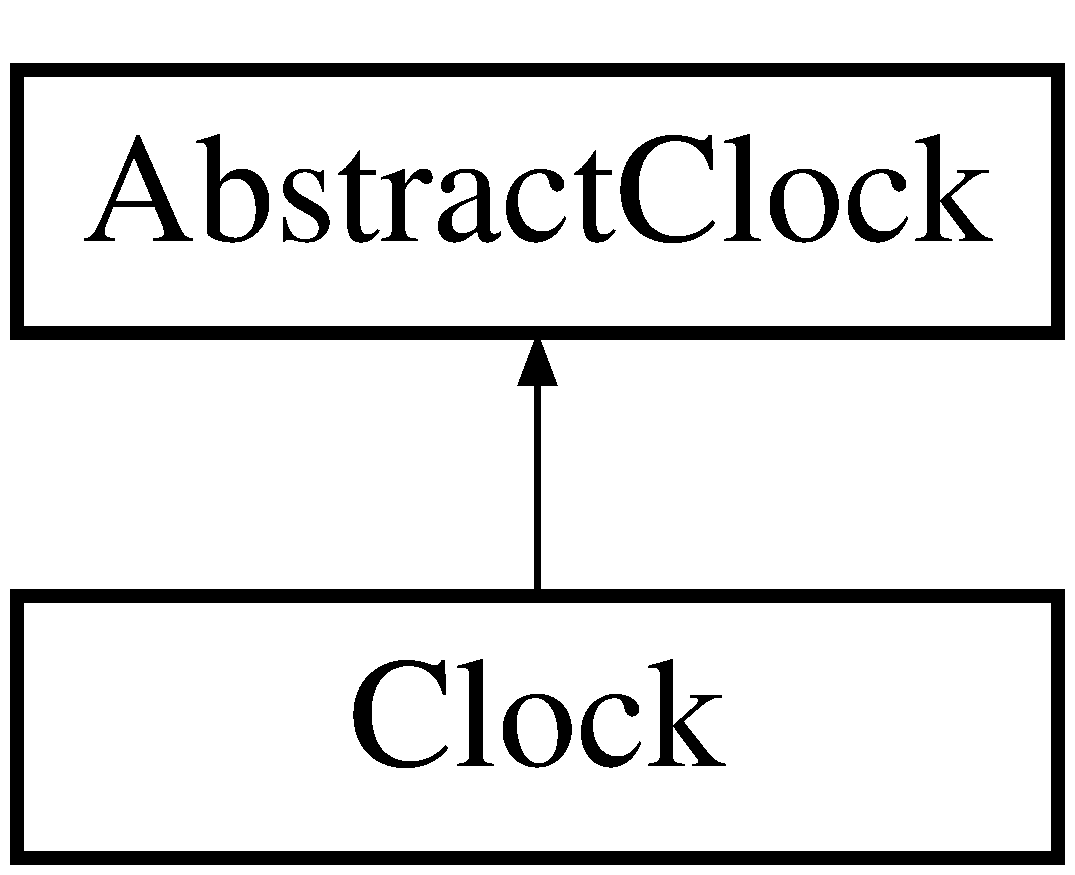
\includegraphics[height=2.000000cm]{classClock}
\end{center}
\end{figure}
\subsection*{Public Member Functions}
\begin{DoxyCompactItemize}
\item 
\hyperlink{classClock_a28d065d80392b50936715f34dfc0b1fc}{Clock} (long int u\_\-abs=0, double u\_\-rel=0)
\begin{DoxyCompactList}\small\item\em constructor giving initial conditions \end{DoxyCompactList}\item 
virtual void \hyperlink{classClock_af0ac46dd780987f2daa69d580e4d5d51}{tick} (unsigned int times=1)
\begin{DoxyCompactList}\small\item\em make the clock tick \end{DoxyCompactList}\item 
\hypertarget{classClock_aca15b58218d8e1a706cbb6217e720267}{
void \hyperlink{classClock_aca15b58218d8e1a706cbb6217e720267}{calculate\_\-relative} ()}
\label{classClock_aca15b58218d8e1a706cbb6217e720267}

\begin{DoxyCompactList}\small\item\em calculate the relative time \end{DoxyCompactList}\item 
\hypertarget{classClock_a1eedc5d52b167ee02f4fe59696bf9d62}{
long int \& \hyperlink{classClock_a1eedc5d52b167ee02f4fe59696bf9d62}{abs} ()}
\label{classClock_a1eedc5d52b167ee02f4fe59696bf9d62}

\begin{DoxyCompactList}\small\item\em set abs \end{DoxyCompactList}\item 
\hypertarget{classClock_af885542ddd8e598b0ced62edcde7f4fa}{
double \& \hyperlink{classClock_af885542ddd8e598b0ced62edcde7f4fa}{rel} ()}
\label{classClock_af885542ddd8e598b0ced62edcde7f4fa}

\begin{DoxyCompactList}\small\item\em set rel \end{DoxyCompactList}\item 
\hypertarget{classClock_a97bb93f3f1f6b6994e7a737ff88ec15d}{
const long int \& \hyperlink{classClock_a97bb93f3f1f6b6994e7a737ff88ec15d}{abs} () const }
\label{classClock_a97bb93f3f1f6b6994e7a737ff88ec15d}

\begin{DoxyCompactList}\small\item\em get abs \end{DoxyCompactList}\item 
\hypertarget{classClock_a7da14c0eb922ca5a4bdffb8159ca7b41}{
const double \& \hyperlink{classClock_a7da14c0eb922ca5a4bdffb8159ca7b41}{rel} () const }
\label{classClock_a7da14c0eb922ca5a4bdffb8159ca7b41}

\begin{DoxyCompactList}\small\item\em get rel \end{DoxyCompactList}\end{DoxyCompactItemize}
\subsection*{Private Attributes}
\begin{DoxyCompactItemize}
\item 
\hypertarget{classClock_a378ea759c6757fe17d11e8636df2da3b}{
long int \hyperlink{classClock_a378ea759c6757fe17d11e8636df2da3b}{m\_\-absolute\_\-time}}
\label{classClock_a378ea759c6757fe17d11e8636df2da3b}

\begin{DoxyCompactList}\small\item\em absolute time \end{DoxyCompactList}\item 
\hypertarget{classClock_a5276273aac712ca2f007c19d80f0f014}{
double \hyperlink{classClock_a5276273aac712ca2f007c19d80f0f014}{m\_\-relative\_\-time}}
\label{classClock_a5276273aac712ca2f007c19d80f0f014}

\begin{DoxyCompactList}\small\item\em relative time \end{DoxyCompactList}\end{DoxyCompactItemize}
\subsection*{Friends}
\begin{DoxyCompactItemize}
\item 
\hypertarget{classClock_a725f3e6c50a193ec896ee00bcc84ce04}{
std::ostream \& \hyperlink{classClock_a725f3e6c50a193ec896ee00bcc84ce04}{operator$<$$<$} (std::ostream \&os, const \hyperlink{classClock}{Clock} \&clock)}
\label{classClock_a725f3e6c50a193ec896ee00bcc84ce04}

\begin{DoxyCompactList}\small\item\em prints the time \end{DoxyCompactList}\end{DoxyCompactItemize}


\subsection{Detailed Description}
real clock able to give the time of the sistem 

give the absolute and relative time of the sistem 

Definition at line 68 of file time.h.



\subsection{Constructor \& Destructor Documentation}
\hypertarget{classClock_a28d065d80392b50936715f34dfc0b1fc}{
\index{Clock@{Clock}!Clock@{Clock}}
\index{Clock@{Clock}!Clock@{Clock}}
\subsubsection[{Clock}]{\setlength{\rightskip}{0pt plus 5cm}Clock::Clock (
\begin{DoxyParamCaption}
\item[{long int}]{u\_\-abs = {\ttfamily 0}, }
\item[{double}]{u\_\-rel = {\ttfamily 0}}
\end{DoxyParamCaption}
)}}
\label{classClock_a28d065d80392b50936715f34dfc0b1fc}


constructor giving initial conditions 

construcor giving the initial absolute time and relative time. default is 0,0


\begin{DoxyParams}{Parameters}
{\em u\_\-abs} & starting absolute time \\
\hline
{\em u\_\-rel} & starting relative time \\
\hline
\end{DoxyParams}


Definition at line 46 of file time.cpp.



\subsection{Member Function Documentation}
\hypertarget{classClock_af0ac46dd780987f2daa69d580e4d5d51}{
\index{Clock@{Clock}!tick@{tick}}
\index{tick@{tick}!Clock@{Clock}}
\subsubsection[{tick}]{\setlength{\rightskip}{0pt plus 5cm}void Clock::tick (
\begin{DoxyParamCaption}
\item[{unsigned int}]{times = {\ttfamily 1}}
\end{DoxyParamCaption}
)\hspace{0.3cm}{\ttfamily  \mbox{[}virtual\mbox{]}}}}
\label{classClock_af0ac46dd780987f2daa69d580e4d5d51}


make the clock tick 

increase the m\_\-absolute time and calculate the relative time 

Implements \hyperlink{classAbstractClock_ad161ad323e50eeba01cc97720a2c469e}{AbstractClock}.



Definition at line 69 of file time.cpp.



The documentation for this class was generated from the following files:\begin{DoxyCompactItemize}
\item 
sources/\hyperlink{time_8h}{time.h}\item 
sources/time.cpp\end{DoxyCompactItemize}

\hypertarget{classeco_1_1Container}{
\section{eco::Container Class Reference}
\label{classeco_1_1Container}\index{eco::Container@{eco::Container}}
}


\hyperlink{classeco_1_1Container}{Container} abstract class.  




{\ttfamily \#include $<$container.h$>$}

Inheritance diagram for eco::Container:\begin{figure}[H]
\begin{center}
\leavevmode
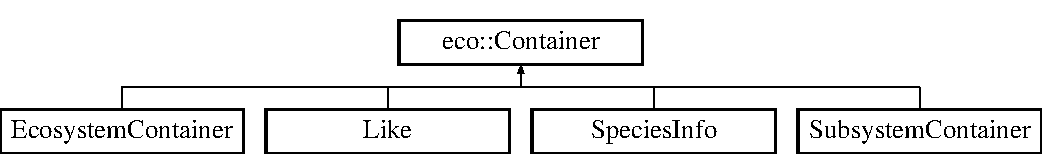
\includegraphics[height=2.000000cm]{classeco_1_1Container}
\end{center}
\end{figure}
\subsection*{Public Member Functions}
\begin{DoxyCompactItemize}
\item 
\hypertarget{classeco_1_1Container_a1b0c5515d6863c1bc98cc93b65952f42}{
\hyperlink{classeco_1_1Container_a1b0c5515d6863c1bc98cc93b65952f42}{Container} ()}
\label{classeco_1_1Container_a1b0c5515d6863c1bc98cc93b65952f42}

\begin{DoxyCompactList}\small\item\em default constructor \end{DoxyCompactList}\item 
\hypertarget{classeco_1_1Container_ae9f5d07bfc3defda274aa06091c19f56}{
\hyperlink{classeco_1_1Container_ae9f5d07bfc3defda274aa06091c19f56}{$\sim$Container} ()}
\label{classeco_1_1Container_ae9f5d07bfc3defda274aa06091c19f56}

\begin{DoxyCompactList}\small\item\em default destructor \end{DoxyCompactList}\item 
virtual bool \hyperlink{classeco_1_1Container_aaba4667933eb47147b319f6daa7da5c2}{is\_\-full} ()=0
\begin{DoxyCompactList}\small\item\em is the container full \end{DoxyCompactList}\end{DoxyCompactItemize}


\subsection{Detailed Description}
\hyperlink{classeco_1_1Container}{Container} abstract class. 

Definition at line 30 of file container.h.



\subsection{Member Function Documentation}
\hypertarget{classeco_1_1Container_aaba4667933eb47147b319f6daa7da5c2}{
\index{eco::Container@{eco::Container}!is\_\-full@{is\_\-full}}
\index{is\_\-full@{is\_\-full}!eco::Container@{eco::Container}}
\subsubsection[{is\_\-full}]{\setlength{\rightskip}{0pt plus 5cm}bool Container::is\_\-full (
\begin{DoxyParamCaption}
{}
\end{DoxyParamCaption}
)\hspace{0.3cm}{\ttfamily  \mbox{[}pure virtual\mbox{]}}}}
\label{classeco_1_1Container_aaba4667933eb47147b319f6daa7da5c2}


is the container full 

abstract member 

Implemented in \hyperlink{classEcosystemContainer_ac2c4ace58f9adbb265f61057420c5565}{EcosystemContainer}, \hyperlink{structLike_a507be8608c74775b568f093e15decbf1}{Like}, \hyperlink{structSpeciesInfo_a3d012834e84c8d878436a739f141f154}{SpeciesInfo}, and \hyperlink{classSubsystemContainer_abad57ab248735fded65abacb908a1b7c}{SubsystemContainer}.



Definition at line 38 of file container.cpp.



The documentation for this class was generated from the following files:\begin{DoxyCompactItemize}
\item 
sources/container.h\item 
sources/container.cpp\end{DoxyCompactItemize}

\hypertarget{classController}{
\section{Controller Class Reference}
\label{classController}\index{Controller@{Controller}}
}


class that generally controll  




{\ttfamily \#include $<$controller.h$>$}

Inheritance diagram for Controller:\begin{figure}[H]
\begin{center}
\leavevmode
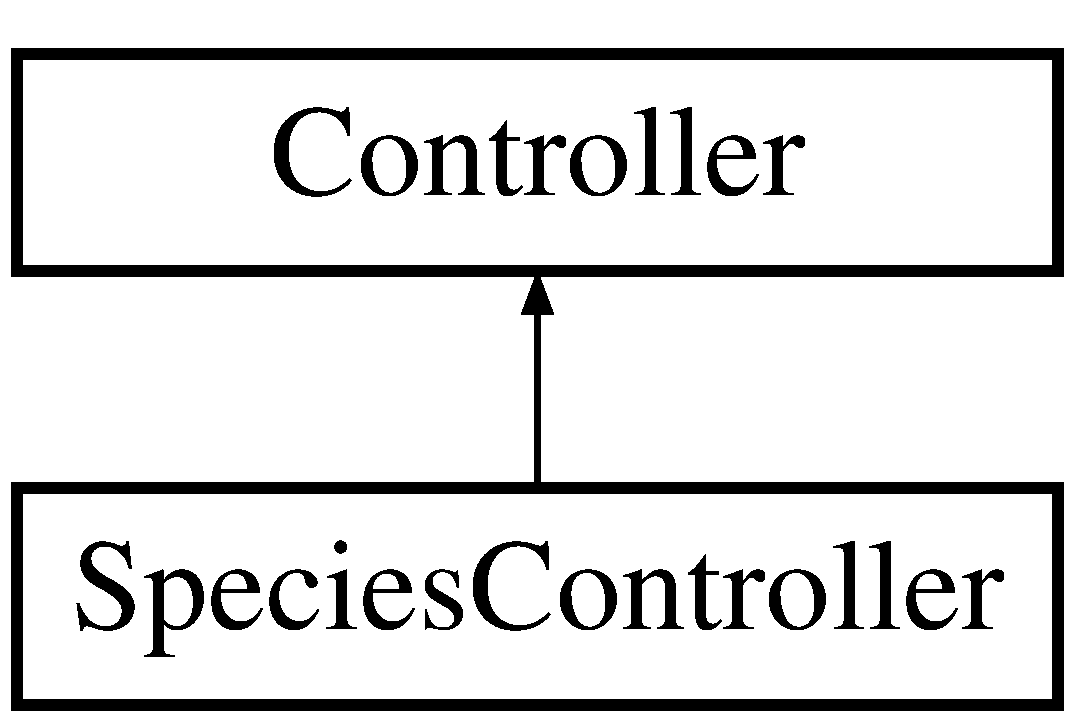
\includegraphics[height=2.000000cm]{classController}
\end{center}
\end{figure}
\subsection*{Public Member Functions}
\begin{DoxyCompactItemize}
\item 
\hypertarget{classController_a29c0a59cb4df6cdde9ee13cd154a2535}{
\hyperlink{classController_a29c0a59cb4df6cdde9ee13cd154a2535}{Controller} ()}
\label{classController_a29c0a59cb4df6cdde9ee13cd154a2535}

\begin{DoxyCompactList}\small\item\em default constructor \end{DoxyCompactList}\item 
\hypertarget{classController_a582aba16637c5c7462e980446b370a22}{
\hyperlink{classController_a582aba16637c5c7462e980446b370a22}{$\sim$Controller} ()}
\label{classController_a582aba16637c5c7462e980446b370a22}

\begin{DoxyCompactList}\small\item\em default destructor \end{DoxyCompactList}\item 
virtual bool \hyperlink{classController_abcf0d0905edc35ee09dc761bd2878d6a}{check} ()=0
\begin{DoxyCompactList}\small\item\em check what is to controll \end{DoxyCompactList}\end{DoxyCompactItemize}


\subsection{Detailed Description}
class that generally controll 

Definition at line 33 of file controller.h.



\subsection{Member Function Documentation}
\hypertarget{classController_abcf0d0905edc35ee09dc761bd2878d6a}{
\index{Controller@{Controller}!check@{check}}
\index{check@{check}!Controller@{Controller}}
\subsubsection[{check}]{\setlength{\rightskip}{0pt plus 5cm}virtual bool Controller::check (
\begin{DoxyParamCaption}
{}
\end{DoxyParamCaption}
)\hspace{0.3cm}{\ttfamily  \mbox{[}pure virtual\mbox{]}}}}
\label{classController_abcf0d0905edc35ee09dc761bd2878d6a}


check what is to controll 

abstarct function 

Implemented in \hyperlink{classSpeciesController_a82ca8bb4c8f99e8b1151990ef293e39a}{SpeciesController}.



The documentation for this class was generated from the following files:\begin{DoxyCompactItemize}
\item 
sources/\hyperlink{controller_8h}{controller.h}\item 
sources/controller.cpp\end{DoxyCompactItemize}

\hypertarget{classDateOfBirth}{
\section{DateOfBirth Class Reference}
\label{classDateOfBirth}\index{DateOfBirth@{DateOfBirth}}
}


simple class for the date of birh  




{\ttfamily \#include $<$time.h$>$}

\subsection*{Public Member Functions}
\begin{DoxyCompactItemize}
\item 
\hyperlink{classDateOfBirth_a2b781b44d207a48f9a17066a54c33bd1}{DateOfBirth} (long int u\_\-abs=0, double u\_\-rel=0)
\begin{DoxyCompactList}\small\item\em default creator \end{DoxyCompactList}\item 
\hyperlink{classDateOfBirth_a858604e5921287e5cb35dcadbff2689c}{DateOfBirth} (const \hyperlink{classClock}{Clock} \&u\_\-clock)
\begin{DoxyCompactList}\small\item\em creator whith a clock \end{DoxyCompactList}\item 
\hypertarget{classDateOfBirth_a9da1d12a3ef90a918bdea5a077e47f89}{
\hyperlink{classDateOfBirth_a9da1d12a3ef90a918bdea5a077e47f89}{$\sim$DateOfBirth} ()}
\label{classDateOfBirth_a9da1d12a3ef90a918bdea5a077e47f89}

\begin{DoxyCompactList}\small\item\em default destructor \end{DoxyCompactList}\item 
\hypertarget{classDateOfBirth_a4abde2ade51debf11060f515c157b658}{
const long int \& \hyperlink{classDateOfBirth_a4abde2ade51debf11060f515c157b658}{abs} () const }
\label{classDateOfBirth_a4abde2ade51debf11060f515c157b658}

\begin{DoxyCompactList}\small\item\em get abs \end{DoxyCompactList}\item 
\hypertarget{classDateOfBirth_a15399ab56a0b32b64d4b4ead601ba657}{
long int \& \hyperlink{classDateOfBirth_a15399ab56a0b32b64d4b4ead601ba657}{abs} ()}
\label{classDateOfBirth_a15399ab56a0b32b64d4b4ead601ba657}

\begin{DoxyCompactList}\small\item\em set abs \end{DoxyCompactList}\item 
\hypertarget{classDateOfBirth_a00324f71b547eb938030effcb5249eb7}{
const double \& \hyperlink{classDateOfBirth_a00324f71b547eb938030effcb5249eb7}{rel} () const }
\label{classDateOfBirth_a00324f71b547eb938030effcb5249eb7}

\begin{DoxyCompactList}\small\item\em get rel \end{DoxyCompactList}\item 
\hypertarget{classDateOfBirth_a3e050eecd8749371d3d8c21d76f146dd}{
double \& \hyperlink{classDateOfBirth_a3e050eecd8749371d3d8c21d76f146dd}{rel} ()}
\label{classDateOfBirth_a3e050eecd8749371d3d8c21d76f146dd}

\begin{DoxyCompactList}\small\item\em set rel \end{DoxyCompactList}\end{DoxyCompactItemize}
\subsection*{Private Attributes}
\begin{DoxyCompactItemize}
\item 
long int \hyperlink{classDateOfBirth_a3f2be0fbfb187a421301d50c768784ba}{m\_\-absolute}
\begin{DoxyCompactList}\small\item\em absolute date of birth \end{DoxyCompactList}\item 
double \hyperlink{classDateOfBirth_a4e0f255eaf334e4e35a49aceee5df28d}{m\_\-relative}
\begin{DoxyCompactList}\small\item\em relative date of birth \end{DoxyCompactList}\end{DoxyCompactItemize}
\subsection*{Friends}
\begin{DoxyCompactItemize}
\item 
\hypertarget{classDateOfBirth_abc2fd3b2388c85ad5f2399f4f250df3a}{
std::ostream \& \hyperlink{classDateOfBirth_abc2fd3b2388c85ad5f2399f4f250df3a}{operator$<$$<$} (std::ostream \&os, const \hyperlink{classDateOfBirth}{DateOfBirth} \&date)}
\label{classDateOfBirth_abc2fd3b2388c85ad5f2399f4f250df3a}

\begin{DoxyCompactList}\small\item\em stream to print the \hyperlink{classDateOfBirth}{DateOfBirth} \end{DoxyCompactList}\end{DoxyCompactItemize}


\subsection{Detailed Description}
simple class for the date of birh 

this class is a simple wrapper that contain the information relatives to the date of life of the form of life. it contains the relative and the absolute date of birth 

Definition at line 122 of file time.h.



\subsection{Constructor \& Destructor Documentation}
\hypertarget{classDateOfBirth_a2b781b44d207a48f9a17066a54c33bd1}{
\index{DateOfBirth@{DateOfBirth}!DateOfBirth@{DateOfBirth}}
\index{DateOfBirth@{DateOfBirth}!DateOfBirth@{DateOfBirth}}
\subsubsection[{DateOfBirth}]{\setlength{\rightskip}{0pt plus 5cm}DateOfBirth::DateOfBirth (
\begin{DoxyParamCaption}
\item[{long int}]{u\_\-abs = {\ttfamily 0}, }
\item[{double}]{u\_\-rel = {\ttfamily 0}}
\end{DoxyParamCaption}
)}}
\label{classDateOfBirth_a2b781b44d207a48f9a17066a54c33bd1}


default creator 

gives all 0 value, not assign clock\_\-ref 

Definition at line 100 of file time.cpp.

\hypertarget{classDateOfBirth_a858604e5921287e5cb35dcadbff2689c}{
\index{DateOfBirth@{DateOfBirth}!DateOfBirth@{DateOfBirth}}
\index{DateOfBirth@{DateOfBirth}!DateOfBirth@{DateOfBirth}}
\subsubsection[{DateOfBirth}]{\setlength{\rightskip}{0pt plus 5cm}DateOfBirth::DateOfBirth (
\begin{DoxyParamCaption}
\item[{const {\bf Clock} \&}]{u\_\-clock}
\end{DoxyParamCaption}
)}}
\label{classDateOfBirth_a858604e5921287e5cb35dcadbff2689c}


creator whith a clock 

set the birth date using the clock you pass it 

Definition at line 108 of file time.cpp.



\subsection{Member Data Documentation}
\hypertarget{classDateOfBirth_a3f2be0fbfb187a421301d50c768784ba}{
\index{DateOfBirth@{DateOfBirth}!m\_\-absolute@{m\_\-absolute}}
\index{m\_\-absolute@{m\_\-absolute}!DateOfBirth@{DateOfBirth}}
\subsubsection[{m\_\-absolute}]{\setlength{\rightskip}{0pt plus 5cm}long int {\bf DateOfBirth::m\_\-absolute}\hspace{0.3cm}{\ttfamily  \mbox{[}private\mbox{]}}}}
\label{classDateOfBirth_a3f2be0fbfb187a421301d50c768784ba}


absolute date of birth 

date of birth expressed as the number of calls occurred before the creation of the form of life 

Definition at line 162 of file time.h.

\hypertarget{classDateOfBirth_a4e0f255eaf334e4e35a49aceee5df28d}{
\index{DateOfBirth@{DateOfBirth}!m\_\-relative@{m\_\-relative}}
\index{m\_\-relative@{m\_\-relative}!DateOfBirth@{DateOfBirth}}
\subsubsection[{m\_\-relative}]{\setlength{\rightskip}{0pt plus 5cm}double {\bf DateOfBirth::m\_\-relative}\hspace{0.3cm}{\ttfamily  \mbox{[}private\mbox{]}}}}
\label{classDateOfBirth_a4e0f255eaf334e4e35a49aceee5df28d}


relative date of birth 

date of birth expressed as number of cicle occurred before the creation of the form of life 

Definition at line 167 of file time.h.



The documentation for this class was generated from the following files:\begin{DoxyCompactItemize}
\item 
sources/\hyperlink{time_8h}{time.h}\item 
sources/time.cpp\end{DoxyCompactItemize}

\hypertarget{structSubsystemContainer_1_1eat}{
\section{SubsystemContainer::eat Struct Reference}
\label{structSubsystemContainer_1_1eat}\index{SubsystemContainer::eat@{SubsystemContainer::eat}}
}


boost multyindex::ordered\_\-index tag  




{\ttfamily \#include $<$subsystemcontainer.h$>$}



\subsection{Detailed Description}
boost multyindex::ordered\_\-index tag 

Definition at line 83 of file subsystemcontainer.h.



The documentation for this struct was generated from the following file:\begin{DoxyCompactItemize}
\item 
sources/\hyperlink{subsystemcontainer_8h}{subsystemcontainer.h}\end{DoxyCompactItemize}

\hypertarget{classEcosystemContainer}{
\section{EcosystemContainer Class Reference}
\label{classEcosystemContainer}\index{EcosystemContainer@{EcosystemContainer}}
}


contains all the form of life  




{\ttfamily \#include $<$ecosystem.h$>$}

Inheritance diagram for EcosystemContainer:\begin{figure}[H]
\begin{center}
\leavevmode
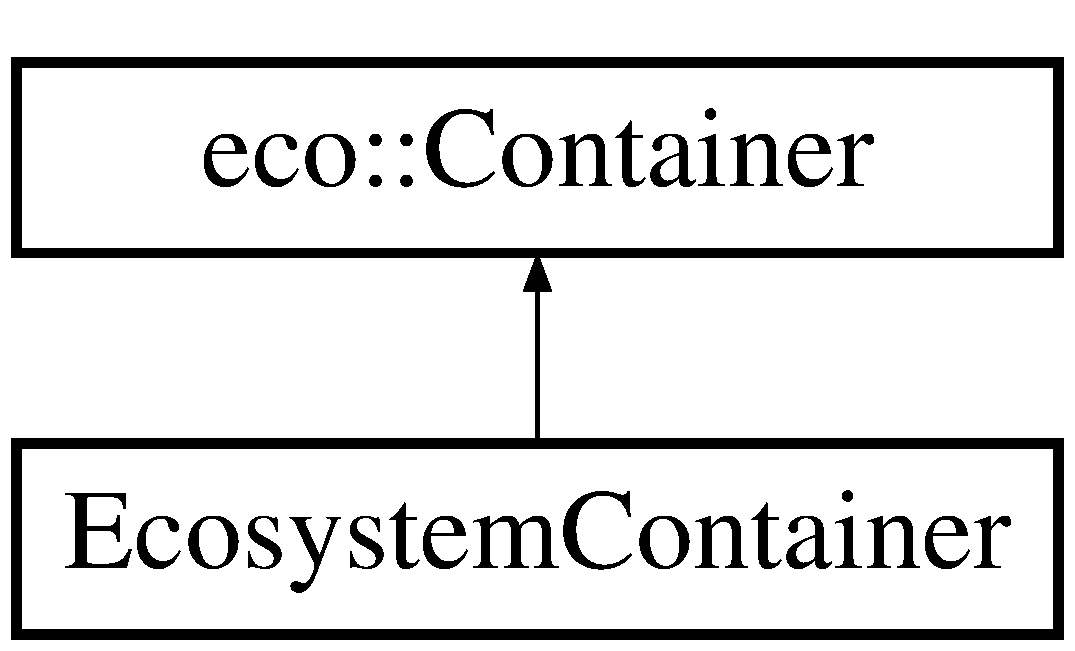
\includegraphics[height=2.000000cm]{classEcosystemContainer}
\end{center}
\end{figure}
\subsection*{Public Types}
\begin{DoxyCompactItemize}
\item 
typedef boost::multi\_\-array$<$ \hyperlink{classSubsystemContainer}{SubsystemContainer}, 2 $>$ \hyperlink{classEcosystemContainer_a52c612c138ad2af06dcf353e6c541345}{ecosys\_\-type}
\begin{DoxyCompactList}\small\item\em the type of the ecosystem is a boost multi\_\-array container \end{DoxyCompactList}\end{DoxyCompactItemize}
\subsection*{Public Member Functions}
\begin{DoxyCompactItemize}
\item 
\hypertarget{classEcosystemContainer_a9eca43f1e0446d7f114e53ccacbe21af}{
\hyperlink{classEcosystemContainer_a9eca43f1e0446d7f114e53ccacbe21af}{EcosystemContainer} (unsigned int u\_\-x\_\-size=0, unsigned int u\_\-y\_\-size=0, bool u\_\-bound=true, unsigned int u\_\-species\_\-number=1, bool u\_\-random\_\-seed=false)}
\label{classEcosystemContainer_a9eca43f1e0446d7f114e53ccacbe21af}

\begin{DoxyCompactList}\small\item\em default constructor \end{DoxyCompactList}\item 
\hypertarget{classEcosystemContainer_aaf7bbc46ec920a24b51732a221bdc537}{
\hyperlink{classEcosystemContainer_aaf7bbc46ec920a24b51732a221bdc537}{$\sim$EcosystemContainer} ()}
\label{classEcosystemContainer_aaf7bbc46ec920a24b51732a221bdc537}

\begin{DoxyCompactList}\small\item\em default destructor \end{DoxyCompactList}\item 
virtual bool \hyperlink{classEcosystemContainer_ac2c4ace58f9adbb265f61057420c5565}{is\_\-full} ()
\begin{DoxyCompactList}\small\item\em is the system full? \end{DoxyCompactList}\item 
void \hyperlink{classEcosystemContainer_a109ceeea2d948bc0d1ef407540cfb52d}{initialize} (std::istream \&is)
\begin{DoxyCompactList}\small\item\em initialize the sistem for the \hyperlink{classEcosystemContainer_a16d9614266ac07dc5252b1e731ab4712}{step()} \end{DoxyCompactList}\item 
void \hyperlink{classEcosystemContainer_a1a77a1d8297bba029bee543bed14f791}{initialize} (std::ifstream \&infs)
\begin{DoxyCompactList}\small\item\em initialize the sistem for \hyperlink{classEcosystemContainer_a16d9614266ac07dc5252b1e731ab4712}{step()} \end{DoxyCompactList}\item 
bool \hyperlink{classEcosystemContainer_a8be87beffab0799737ac8fe5091a9ff3}{insert} (\hyperlink{classIndividualAnimal}{IndividualAnimal} \&u\_\-an, const int u\_\-x, const int u\_\-y)
\begin{DoxyCompactList}\small\item\em insert animal in subecosystem container \end{DoxyCompactList}\item 
bool \hyperlink{classEcosystemContainer_a2ca198ce9aeb2082a9d5b76de4d0b45c}{insert} (\hyperlink{classIndividualVegetable}{IndividualVegetable} \&u\_\-veg, const int u\_\-x, const int u\_\-y)
\begin{DoxyCompactList}\small\item\em insert vegetable in the ecosystem container \end{DoxyCompactList}\item 
bool \hyperlink{classEcosystemContainer_a16d9614266ac07dc5252b1e731ab4712}{step} ()
\begin{DoxyCompactList}\small\item\em step evolution \end{DoxyCompactList}\item 
bool \hyperlink{classEcosystemContainer_a236c01266343664efab29b1a73e72d1d}{step} (\hyperlink{structStepLog}{StepLog} \&log)
\begin{DoxyCompactList}\small\item\em step evoultion producing steplog \end{DoxyCompactList}\item 
void \hyperlink{classEcosystemContainer_acc91c956fd0afc63a055c7072e250914}{FillRandom} ()
\begin{DoxyCompactList}\small\item\em fill random ecosystem \end{DoxyCompactList}\item 
\hypertarget{classEcosystemContainer_a248efcbe5e1cb7d4da1916df27e05520}{
bool \hyperlink{classEcosystemContainer_a248efcbe5e1cb7d4da1916df27e05520}{fill} (std::ifstream \&ifs)}
\label{classEcosystemContainer_a248efcbe5e1cb7d4da1916df27e05520}

\begin{DoxyCompactList}\small\item\em fill the ecosystem from a file \end{DoxyCompactList}\item 
std::pair$<$ unsigned int, bool $>$ \hyperlink{classEcosystemContainer_a5330060eabcdf726931e3c8984a71073}{specied\_\-population} (const unsigned int u\_\-spec\_\-id=0)
\begin{DoxyCompactList}\small\item\em total number of specied of this species \end{DoxyCompactList}\item 
void \hyperlink{classEcosystemContainer_a8f3fecee71e06e35a32ec35e3c01f924}{draw\_\-evolv} (const unsigned int steps)
\begin{DoxyCompactList}\small\item\em draw and evolv \end{DoxyCompactList}\item 
void \hyperlink{classEcosystemContainer_a9aedfda6204c1569234bf41489b88bd4}{draw\_\-evolv\_\-fast} (const unsigned int steps, std::string options=std::string(\char`\"{}refresh\_\-populations\char`\"{}))
\begin{DoxyCompactList}\small\item\em draw the evolution of the system in a fast way \end{DoxyCompactList}\item 
bool \hyperlink{classEcosystemContainer_a37e7e126c7ee9855a4fa3218711a5b1d}{evolv} (unsigned int steps)
\begin{DoxyCompactList}\small\item\em make the system evolv \end{DoxyCompactList}\item 
bool \hyperlink{classEcosystemContainer_a257157a8dbe84b0f5abcbde4fab0c9ae}{evolv} (unsigned int steps, std::vector$<$ \hyperlink{structStepLog}{StepLog} $>$ \&logs)
\begin{DoxyCompactList}\small\item\em make the system evolv and create a log \end{DoxyCompactList}\item 
bool \hyperlink{classEcosystemContainer_acbdecb83a3b8b0f4433b0a01a04d7af4}{evolv} (unsigned int steps, std::ofstream \&ofs)
\begin{DoxyCompactList}\small\item\em evolv the system and write logs \end{DoxyCompactList}\item 
\hypertarget{classEcosystemContainer_a6e175385de623dcbc018e5d8ae5c8af4}{
\hyperlink{classEcosystemContainer_a52c612c138ad2af06dcf353e6c541345}{ecosys\_\-type} \& \hyperlink{classEcosystemContainer_a6e175385de623dcbc018e5d8ae5c8af4}{ecosystem} ()}
\label{classEcosystemContainer_a6e175385de623dcbc018e5d8ae5c8af4}

\begin{DoxyCompactList}\small\item\em set the ecosystem \end{DoxyCompactList}\item 
\hyperlink{classSubsystemContainer}{SubsystemContainer} \& \hyperlink{classEcosystemContainer_a3a908f8550a2800227774a0fe623593c}{subsystem} (const int u\_\-x, const int u\_\-y)
\begin{DoxyCompactList}\small\item\em set the \hyperlink{classSubsystemContainer}{SubsystemContainer} \end{DoxyCompactList}\item 
\hypertarget{classEcosystemContainer_aa23780e2602c9aea376390c309261288}{
const \hyperlink{classEcosystemContainer_a52c612c138ad2af06dcf353e6c541345}{ecosys\_\-type} \& \hyperlink{classEcosystemContainer_aa23780e2602c9aea376390c309261288}{ecosystem} () const }
\label{classEcosystemContainer_aa23780e2602c9aea376390c309261288}

\begin{DoxyCompactList}\small\item\em get the ecosystem \end{DoxyCompactList}\item 
const \hyperlink{classSubsystemContainer}{SubsystemContainer} \& \hyperlink{classEcosystemContainer_a957ab87f64f41f8c1669f993c1976a85}{subsystem} (int u\_\-x, int u\_\-y) const 
\begin{DoxyCompactList}\small\item\em get the \hyperlink{classSubsystemContainer}{SubsystemContainer} \end{DoxyCompactList}\end{DoxyCompactItemize}
\subsection*{Private Member Functions}
\begin{DoxyCompactItemize}
\item 
std::pair$<$ bool, bool $>$ \hyperlink{classEcosystemContainer_a1f8ef307d02139dd3483933057478dfd}{m\_\-newborn} (const unsigned int species\_\-id, const unsigned int subs\_\-x, const unsigned int subs\_\-y, unsigned int u\_\-hp)
\begin{DoxyCompactList}\small\item\em create a newborn for the species indicated \end{DoxyCompactList}\item 
std::pair$<$ bool, bool $>$ \hyperlink{classEcosystemContainer_a38c68130f0005de72f8f0ba01bb29472}{m\_\-newborn} (const unsigned int species\_\-id, const unsigned int subs\_\-x, const unsigned int subs\_\-y, unsigned int u\_\-hp, \hyperlink{structStepLog}{StepLog} \&log)
\begin{DoxyCompactList}\small\item\em create a newborn for the species indicated \end{DoxyCompactList}\item 
int \hyperlink{classEcosystemContainer_ad046555c1a42891ea1ceb14fe3a2bed5}{m\_\-rand\_\-int} (int a=0, int b=0)
\begin{DoxyCompactList}\small\item\em get a random int \end{DoxyCompactList}\item 
void \hyperlink{classEcosystemContainer_a8c82bc02305c597ce40914491fbb8aec}{m\_\-dead} (\hyperlink{classSubsystemContainer_a90723cf9f8cdae39e46ff65c5c898c2c}{SubsystemContainer::an\_\-eat\_\-it} dead\_\-an, \hyperlink{classSubsystemContainer_ad6392db27e78a340c21252e63edbe55f}{SubsystemContainer::index\_\-an\_\-by\_\-eat} \&eat\_\-index)
\begin{DoxyCompactList}\small\item\em remove animal from the index provided \end{DoxyCompactList}\item 
void \hyperlink{classEcosystemContainer_a803abe3366ba3d8579a92efc1096a2a6}{m\_\-dead} (\hyperlink{classSubsystemContainer_a90723cf9f8cdae39e46ff65c5c898c2c}{SubsystemContainer::an\_\-eat\_\-it} dead\_\-an, \hyperlink{classSubsystemContainer_ad6392db27e78a340c21252e63edbe55f}{SubsystemContainer::index\_\-an\_\-by\_\-eat} \&eat\_\-index, \hyperlink{structStepLog}{StepLog} \&log, int x, int y)
\begin{DoxyCompactList}\small\item\em remove animal from the index provided and create a log \end{DoxyCompactList}\item 
void \hyperlink{classEcosystemContainer_ac20491928d3df161e621586a282b8e04}{m\_\-dead} (\hyperlink{classSubsystemContainer_a016775688f9d4baed66e8bdc3fbc0ec9}{SubsystemContainer::an\_\-id\_\-it} dead\_\-an, \hyperlink{classSubsystemContainer_ae095d19ad8aee4e1f1620166f440cf99}{SubsystemContainer::index\_\-an\_\-by\_\-id} \&id\_\-index)
\begin{DoxyCompactList}\small\item\em remove animal from the index provided \end{DoxyCompactList}\item 
void \hyperlink{classEcosystemContainer_a308e43a136e8990d4229dbdd6a8bfa56}{m\_\-dead} (\hyperlink{classSubsystemContainer_a016775688f9d4baed66e8bdc3fbc0ec9}{SubsystemContainer::an\_\-id\_\-it} dead\_\-an, \hyperlink{classSubsystemContainer_ae095d19ad8aee4e1f1620166f440cf99}{SubsystemContainer::index\_\-an\_\-by\_\-id} \&id\_\-index, \hyperlink{structStepLog}{StepLog} \&log, int x, int y)
\begin{DoxyCompactList}\small\item\em remove animal from the index provided and create a log \end{DoxyCompactList}\item 
void \hyperlink{classEcosystemContainer_a76a30d59c284f91c5df800631b9acd0a}{m\_\-dead} (\hyperlink{classSubsystemContainer_aee4873426aef4e4f9f8d41ffb2b2f781}{SubsystemContainer::an\_\-reproduce\_\-it} dead\_\-an, \hyperlink{classSubsystemContainer_a08f08e93dceda155601c8ff6ed31839e}{SubsystemContainer::index\_\-an\_\-by\_\-reproduce} \&repr\_\-index)
\begin{DoxyCompactList}\small\item\em remove animal from the index provided \end{DoxyCompactList}\item 
void \hyperlink{classEcosystemContainer_ab9766e2ce58e850fa2764e07027f88db}{m\_\-dead} (\hyperlink{classSubsystemContainer_aee4873426aef4e4f9f8d41ffb2b2f781}{SubsystemContainer::an\_\-reproduce\_\-it} dead\_\-an, \hyperlink{classSubsystemContainer_a08f08e93dceda155601c8ff6ed31839e}{SubsystemContainer::index\_\-an\_\-by\_\-reproduce} \&repr\_\-index, \hyperlink{structStepLog}{StepLog} \&log, int x, int y)
\begin{DoxyCompactList}\small\item\em remove animal from the index provided and create a log \end{DoxyCompactList}\item 
void \hyperlink{classEcosystemContainer_a18d6b66ba403b00cbb3069bfcc2a72d6}{m\_\-bound\_\-translator} (int \&x, int \&y)
\begin{DoxyCompactList}\small\item\em translate the coordinate if there were no boundaries \end{DoxyCompactList}\item 
bool \hyperlink{classEcosystemContainer_a1f17cee83b62c0b3a088701011a09f0d}{m\_\-where\_\-to\_\-move} (int \&u\_\-x, int \&u\_\-y, const int curr\_\-x, const int curr\_\-y, const unsigned int species\_\-id)
\begin{DoxyCompactList}\small\item\em where an animal could move \end{DoxyCompactList}\item 
bool \hyperlink{classEcosystemContainer_af1b88c429ba4807eaa02c1c958a8037c}{m\_\-migrate} (const int curr\_\-x, const int curr\_\-y, \hyperlink{classSubsystemContainer_a016775688f9d4baed66e8bdc3fbc0ec9}{SubsystemContainer::an\_\-id\_\-it} \&to\_\-move, \hyperlink{classSubsystemContainer_ae095d19ad8aee4e1f1620166f440cf99}{SubsystemContainer::index\_\-an\_\-by\_\-id} \&idx)
\begin{DoxyCompactList}\small\item\em migrate form curr\_\-x and curr\_\-y using m\_\-where\_\-to\_\-move \end{DoxyCompactList}\item 
bool \hyperlink{classEcosystemContainer_af383cbfff979511fa2d88776d5058185}{m\_\-migrate} (const int curr\_\-x, const int curr\_\-y, \hyperlink{classSubsystemContainer_a016775688f9d4baed66e8bdc3fbc0ec9}{SubsystemContainer::an\_\-id\_\-it} \&to\_\-move, \hyperlink{classSubsystemContainer_ae095d19ad8aee4e1f1620166f440cf99}{SubsystemContainer::index\_\-an\_\-by\_\-id} \&idx, \hyperlink{structStepLog}{StepLog} \&log)
\begin{DoxyCompactList}\small\item\em migrate form curr\_\-x and curr\_\-y using m\_\-where\_\-to\_\-move \end{DoxyCompactList}\end{DoxyCompactItemize}
\subsection*{Private Attributes}
\begin{DoxyCompactItemize}
\item 
\hypertarget{classEcosystemContainer_a61ee14b3ace1c7a1548c7dcffbdd4fc2}{
unsigned int \hyperlink{classEcosystemContainer_a61ee14b3ace1c7a1548c7dcffbdd4fc2}{m\_\-x\_\-size}}
\label{classEcosystemContainer_a61ee14b3ace1c7a1548c7dcffbdd4fc2}

\begin{DoxyCompactList}\small\item\em x size of the container \end{DoxyCompactList}\item 
\hypertarget{classEcosystemContainer_ae6b6c3cfeb86973490c1e4bf37c6712b}{
unsigned int \hyperlink{classEcosystemContainer_ae6b6c3cfeb86973490c1e4bf37c6712b}{m\_\-y\_\-size}}
\label{classEcosystemContainer_ae6b6c3cfeb86973490c1e4bf37c6712b}

\begin{DoxyCompactList}\small\item\em y size of the container \end{DoxyCompactList}\item 
\hypertarget{classEcosystemContainer_a87d7a3c084c9f8ed29a7484c91a9ebb9}{
bool \hyperlink{classEcosystemContainer_a87d7a3c084c9f8ed29a7484c91a9ebb9}{m\_\-boundaries}}
\label{classEcosystemContainer_a87d7a3c084c9f8ed29a7484c91a9ebb9}

\begin{DoxyCompactList}\small\item\em if the ecosystem have boundaries or not \end{DoxyCompactList}\item 
\hyperlink{classEcosystemContainer_a52c612c138ad2af06dcf353e6c541345}{ecosys\_\-type} \hyperlink{classEcosystemContainer_a19f047377f131b497c7258b58adb1a45}{m\_\-ecosystem}
\begin{DoxyCompactList}\small\item\em the ecosystem as ensable of subsystem containers \end{DoxyCompactList}\item 
unsigned long int \hyperlink{classEcosystemContainer_adefb24e46962eab1528a2fc322ae6e53}{m\_\-last\_\-existance\_\-id}
\begin{DoxyCompactList}\small\item\em the last existance id of a new creature \end{DoxyCompactList}\item 
\hyperlink{classSpeciesController}{SpeciesController} \hyperlink{classEcosystemContainer_a41211c58341df2a0ef7ee44b69151de0}{m\_\-species\_\-controller}
\begin{DoxyCompactList}\small\item\em the species controller for this ecosys \end{DoxyCompactList}\item 
\hypertarget{classEcosystemContainer_aaf112f8024a548d0266bd4b87653c2f8}{
\hyperlink{classClock}{Clock} \hyperlink{classEcosystemContainer_aaf112f8024a548d0266bd4b87653c2f8}{m\_\-clock}}
\label{classEcosystemContainer_aaf112f8024a548d0266bd4b87653c2f8}

\begin{DoxyCompactList}\small\item\em the clock of the system \end{DoxyCompactList}\item 
\hypertarget{classEcosystemContainer_aa6403dd5bcafef13d4f696f3f8c4f52a}{
boost::mt19937 \hyperlink{classEcosystemContainer_aa6403dd5bcafef13d4f696f3f8c4f52a}{m\_\-generator}}
\label{classEcosystemContainer_aa6403dd5bcafef13d4f696f3f8c4f52a}

\begin{DoxyCompactList}\small\item\em the random number generator used by m\_\-rand\_\-int \end{DoxyCompactList}\end{DoxyCompactItemize}
\subsection*{Friends}
\begin{DoxyCompactItemize}
\item 
\hypertarget{classEcosystemContainer_a8863e5007c8cf23c4b14342c947cc1eb}{
std::ifstream \& {\bfseries operator$>$$>$} (std::ifstream \&is, \hyperlink{classEcosystemContainer}{EcosystemContainer} \&eco)}
\label{classEcosystemContainer_a8863e5007c8cf23c4b14342c947cc1eb}

\end{DoxyCompactItemize}


\subsection{Detailed Description}
contains all the form of life 

Definition at line 49 of file ecosystem.h.



\subsection{Member Typedef Documentation}
\hypertarget{classEcosystemContainer_a52c612c138ad2af06dcf353e6c541345}{
\index{EcosystemContainer@{EcosystemContainer}!ecosys\_\-type@{ecosys\_\-type}}
\index{ecosys\_\-type@{ecosys\_\-type}!EcosystemContainer@{EcosystemContainer}}
\subsubsection[{ecosys\_\-type}]{\setlength{\rightskip}{0pt plus 5cm}typedef boost::multi\_\-array$<${\bf SubsystemContainer}, 2$>$ {\bf EcosystemContainer::ecosys\_\-type}}}
\label{classEcosystemContainer_a52c612c138ad2af06dcf353e6c541345}


the type of the ecosystem is a boost multi\_\-array container 

roughtly is a matrix 

Definition at line 55 of file ecosystem.h.



\subsection{Member Function Documentation}
\hypertarget{classEcosystemContainer_a8f3fecee71e06e35a32ec35e3c01f924}{
\index{EcosystemContainer@{EcosystemContainer}!draw\_\-evolv@{draw\_\-evolv}}
\index{draw\_\-evolv@{draw\_\-evolv}!EcosystemContainer@{EcosystemContainer}}
\subsubsection[{draw\_\-evolv}]{\setlength{\rightskip}{0pt plus 5cm}void Eco::draw\_\-evolv (
\begin{DoxyParamCaption}
\item[{const unsigned int}]{steps}
\end{DoxyParamCaption}
)}}
\label{classEcosystemContainer_a8f3fecee71e06e35a32ec35e3c01f924}


draw and evolv 

evolv the sistem for a number of steps and draw his evolution this method is slower than draw\_\-evolv\_\-fast because for every step it reset the TH2F and compute the total population for every species in every single subsystem. although the rappresentation is always right. 

Definition at line 61 of file draw\_\-evolv.cpp.

\hypertarget{classEcosystemContainer_a9aedfda6204c1569234bf41489b88bd4}{
\index{EcosystemContainer@{EcosystemContainer}!draw\_\-evolv\_\-fast@{draw\_\-evolv\_\-fast}}
\index{draw\_\-evolv\_\-fast@{draw\_\-evolv\_\-fast}!EcosystemContainer@{EcosystemContainer}}
\subsubsection[{draw\_\-evolv\_\-fast}]{\setlength{\rightskip}{0pt plus 5cm}void Eco::draw\_\-evolv\_\-fast (
\begin{DoxyParamCaption}
\item[{const unsigned int}]{steps, }
\item[{std::string}]{options = {\ttfamily std::string(\char`\"{}refresh\_\-populations\char`\"{})}}
\end{DoxyParamCaption}
)}}
\label{classEcosystemContainer_a9aedfda6204c1569234bf41489b88bd4}


draw the evolution of the system in a fast way 

the system will evolv and for each step will be draw something according to options parameter. this method is faster than draw\_\-evolv because it parses the log produced by step( StepLog) and modify the rappresentation whithout performing a query for every subsystem and for every species. it doesn't reset the TH2F but only modify the wheight of the interested bins 

Definition at line 352 of file draw\_\-evolv.cpp.

\hypertarget{classEcosystemContainer_a37e7e126c7ee9855a4fa3218711a5b1d}{
\index{EcosystemContainer@{EcosystemContainer}!evolv@{evolv}}
\index{evolv@{evolv}!EcosystemContainer@{EcosystemContainer}}
\subsubsection[{evolv}]{\setlength{\rightskip}{0pt plus 5cm}bool Eco::evolv (
\begin{DoxyParamCaption}
\item[{unsigned int}]{steps}
\end{DoxyParamCaption}
)}}
\label{classEcosystemContainer_a37e7e126c7ee9855a4fa3218711a5b1d}


make the system evolv 


\begin{DoxyParams}{Parameters}
{\em steps} & number times \hyperlink{classEcosystemContainer_a16d9614266ac07dc5252b1e731ab4712}{step()} will be runned \\
\hline
\end{DoxyParams}
\begin{DoxyReturn}{Returns}
false if step fails. 
\end{DoxyReturn}


Definition at line 1362 of file ecosystem.cpp.

\hypertarget{classEcosystemContainer_a257157a8dbe84b0f5abcbde4fab0c9ae}{
\index{EcosystemContainer@{EcosystemContainer}!evolv@{evolv}}
\index{evolv@{evolv}!EcosystemContainer@{EcosystemContainer}}
\subsubsection[{evolv}]{\setlength{\rightskip}{0pt plus 5cm}bool Eco::evolv (
\begin{DoxyParamCaption}
\item[{unsigned int}]{steps, }
\item[{std::vector$<$ {\bf StepLog} $>$ \&}]{logs}
\end{DoxyParamCaption}
)}}
\label{classEcosystemContainer_a257157a8dbe84b0f5abcbde4fab0c9ae}


make the system evolv and create a log 


\begin{DoxyParams}{Parameters}
{\em steps} & number times \hyperlink{classEcosystemContainer_a16d9614266ac07dc5252b1e731ab4712}{step()} will be runned \\
\hline
{\em Logs} & a vector of \hyperlink{structStepLog}{StepLog} \\
\hline
\end{DoxyParams}
\begin{DoxyReturn}{Returns}
false if step fails. 
\end{DoxyReturn}
\begin{DoxySeeAlso}{See also}
\hyperlink{structStepLog}{StepLog} 
\end{DoxySeeAlso}


Definition at line 1384 of file ecosystem.cpp.

\hypertarget{classEcosystemContainer_acbdecb83a3b8b0f4433b0a01a04d7af4}{
\index{EcosystemContainer@{EcosystemContainer}!evolv@{evolv}}
\index{evolv@{evolv}!EcosystemContainer@{EcosystemContainer}}
\subsubsection[{evolv}]{\setlength{\rightskip}{0pt plus 5cm}bool Eco::evolv (
\begin{DoxyParamCaption}
\item[{unsigned int}]{steps, }
\item[{std::ofstream \&}]{ofs}
\end{DoxyParamCaption}
)}}
\label{classEcosystemContainer_acbdecb83a3b8b0f4433b0a01a04d7af4}


evolv the system and write logs 

evolv the system and once finisched or once \hyperlink{classEcosystemContainer_a16d9614266ac07dc5252b1e731ab4712}{step()} returns false; write using the ofs to a file the results. results are elaborations of \hyperlink{structStepLog}{StepLog} 
\begin{DoxyParams}{Parameters}
{\em steps} & number times \hyperlink{classEcosystemContainer_a16d9614266ac07dc5252b1e731ab4712}{step()} will be runned \\
\hline
{\em ofs} & output file stream in which buffer \\
\hline
\end{DoxyParams}
\begin{DoxyReturn}{Returns}
false if step fails. 
\end{DoxyReturn}


Definition at line 1411 of file ecosystem.cpp.

\hypertarget{classEcosystemContainer_acc91c956fd0afc63a055c7072e250914}{
\index{EcosystemContainer@{EcosystemContainer}!FillRandom@{FillRandom}}
\index{FillRandom@{FillRandom}!EcosystemContainer@{EcosystemContainer}}
\subsubsection[{FillRandom}]{\setlength{\rightskip}{0pt plus 5cm}void Eco::FillRandom (
\begin{DoxyParamCaption}
{}
\end{DoxyParamCaption}
)}}
\label{classEcosystemContainer_acc91c956fd0afc63a055c7072e250914}


fill random ecosystem 

each subsystem will be filled by a random number of vivent for each species whith random hp and random sex. the distribution is uniform and linear. this filling method respect the \hyperlink{classSubsystemContainer_abad57ab248735fded65abacb908a1b7c}{SubsystemContainer::is\_\-full}.

this method is written ad FillRandom and not fillrandom just to do a tribute to root-\/cern lib. 

Definition at line 357 of file ecosystem.cpp.

\hypertarget{classEcosystemContainer_a109ceeea2d948bc0d1ef407540cfb52d}{
\index{EcosystemContainer@{EcosystemContainer}!initialize@{initialize}}
\index{initialize@{initialize}!EcosystemContainer@{EcosystemContainer}}
\subsubsection[{initialize}]{\setlength{\rightskip}{0pt plus 5cm}void Eco::initialize (
\begin{DoxyParamCaption}
\item[{std::istream \&}]{is}
\end{DoxyParamCaption}
)}}
\label{classEcosystemContainer_a109ceeea2d948bc0d1ef407540cfb52d}


initialize the sistem for the \hyperlink{classEcosystemContainer_a16d9614266ac07dc5252b1e731ab4712}{step()} 


\begin{DoxyParams}{Parameters}
{\em is} & generical input stream \\
\hline
\end{DoxyParams}
\begin{DoxyReturn}{Returns}
true if initialization suceed, false if fails 
\end{DoxyReturn}


Definition at line 125 of file ecosystem.cpp.

\hypertarget{classEcosystemContainer_a1a77a1d8297bba029bee543bed14f791}{
\index{EcosystemContainer@{EcosystemContainer}!initialize@{initialize}}
\index{initialize@{initialize}!EcosystemContainer@{EcosystemContainer}}
\subsubsection[{initialize}]{\setlength{\rightskip}{0pt plus 5cm}void Eco::initialize (
\begin{DoxyParamCaption}
\item[{std::ifstream \&}]{infs}
\end{DoxyParamCaption}
)}}
\label{classEcosystemContainer_a1a77a1d8297bba029bee543bed14f791}


initialize the sistem for \hyperlink{classEcosystemContainer_a16d9614266ac07dc5252b1e731ab4712}{step()} 


\begin{DoxyParams}{Parameters}
{\em infs} & input file stream \\
\hline
\end{DoxyParams}
\begin{DoxyReturn}{Returns}
true if initialization suceed, false if fails 
\end{DoxyReturn}


Definition at line 173 of file ecosystem.cpp.

\hypertarget{classEcosystemContainer_a8be87beffab0799737ac8fe5091a9ff3}{
\index{EcosystemContainer@{EcosystemContainer}!insert@{insert}}
\index{insert@{insert}!EcosystemContainer@{EcosystemContainer}}
\subsubsection[{insert}]{\setlength{\rightskip}{0pt plus 5cm}bool Eco::insert (
\begin{DoxyParamCaption}
\item[{{\bf IndividualAnimal} \&}]{u\_\-an, }
\item[{const int}]{u\_\-x, }
\item[{const int}]{u\_\-y}
\end{DoxyParamCaption}
)}}
\label{classEcosystemContainer_a8be87beffab0799737ac8fe5091a9ff3}


insert animal in subecosystem container 


\begin{DoxyParams}{Parameters}
{\em u\_\-an} & the animal to inser \\
\hline
{\em u\_\-x} & the x coord of the subsystem you want to insert in \\
\hline
{\em u\_\-y} & the y coord of the subsystem you want to insert in \\
\hline
\end{DoxyParams}
\begin{DoxyReturn}{Returns}
true if insertion succed, false if fails 
\end{DoxyReturn}


Definition at line 243 of file ecosystem.cpp.

\hypertarget{classEcosystemContainer_a2ca198ce9aeb2082a9d5b76de4d0b45c}{
\index{EcosystemContainer@{EcosystemContainer}!insert@{insert}}
\index{insert@{insert}!EcosystemContainer@{EcosystemContainer}}
\subsubsection[{insert}]{\setlength{\rightskip}{0pt plus 5cm}bool Eco::insert (
\begin{DoxyParamCaption}
\item[{{\bf IndividualVegetable} \&}]{u\_\-veg, }
\item[{const int}]{u\_\-x, }
\item[{const int}]{u\_\-y}
\end{DoxyParamCaption}
)}}
\label{classEcosystemContainer_a2ca198ce9aeb2082a9d5b76de4d0b45c}


insert vegetable in the ecosystem container 


\begin{DoxyParams}{Parameters}
{\em u\_\-veg} & the vegetable to insert \\
\hline
{\em u\_\-x} & the x coord of the subsystem you want to insert in \\
\hline
{\em u\_\-y} & the y coord of the subsystem you want to insert in \\
\hline
\end{DoxyParams}
\begin{DoxyReturn}{Returns}
true if insertion succed, false if fails 
\end{DoxyReturn}


Definition at line 300 of file ecosystem.cpp.

\hypertarget{classEcosystemContainer_ac2c4ace58f9adbb265f61057420c5565}{
\index{EcosystemContainer@{EcosystemContainer}!is\_\-full@{is\_\-full}}
\index{is\_\-full@{is\_\-full}!EcosystemContainer@{EcosystemContainer}}
\subsubsection[{is\_\-full}]{\setlength{\rightskip}{0pt plus 5cm}bool Eco::is\_\-full (
\begin{DoxyParamCaption}
{}
\end{DoxyParamCaption}
)\hspace{0.3cm}{\ttfamily  \mbox{[}virtual\mbox{]}}}}
\label{classEcosystemContainer_ac2c4ace58f9adbb265f61057420c5565}


is the system full? 

\begin{Desc}
\item[\hyperlink{todo__todo000001}{Todo}]implement \end{Desc}


Implements \hyperlink{classeco_1_1Container_aaba4667933eb47147b319f6daa7da5c2}{eco::Container}.



Definition at line 92 of file ecosystem.cpp.

\hypertarget{classEcosystemContainer_a18d6b66ba403b00cbb3069bfcc2a72d6}{
\index{EcosystemContainer@{EcosystemContainer}!m\_\-bound\_\-translator@{m\_\-bound\_\-translator}}
\index{m\_\-bound\_\-translator@{m\_\-bound\_\-translator}!EcosystemContainer@{EcosystemContainer}}
\subsubsection[{m\_\-bound\_\-translator}]{\setlength{\rightskip}{0pt plus 5cm}void Eco::m\_\-bound\_\-translator (
\begin{DoxyParamCaption}
\item[{int \&}]{x, }
\item[{int \&}]{y}
\end{DoxyParamCaption}
)\hspace{0.3cm}{\ttfamily  \mbox{[}private\mbox{]}}}}
\label{classEcosystemContainer_a18d6b66ba403b00cbb3069bfcc2a72d6}


translate the coordinate if there were no boundaries 

if there were no boundaries the x and y coord could be more than m\_\-x\_\-size or m\_\-y\_\-size or less than 0. this function provide a translation of such numbers in an interval from 0 -\/ m\_\-x/y\_\-size.

if the m\_\-boundaries flag is not true and the coordinates are not in the interval it will print an error message and set both x and y to 0 example: if x = m\_\-x\_\-size+1 it becomes 0 

Definition at line 794 of file ecosystem.cpp.

\hypertarget{classEcosystemContainer_ac20491928d3df161e621586a282b8e04}{
\index{EcosystemContainer@{EcosystemContainer}!m\_\-dead@{m\_\-dead}}
\index{m\_\-dead@{m\_\-dead}!EcosystemContainer@{EcosystemContainer}}
\subsubsection[{m\_\-dead}]{\setlength{\rightskip}{0pt plus 5cm}void Eco::m\_\-dead (
\begin{DoxyParamCaption}
\item[{{\bf SubsystemContainer::an\_\-id\_\-it}}]{dead\_\-an, }
\item[{{\bf SubsystemContainer::index\_\-an\_\-by\_\-id} \&}]{id\_\-index}
\end{DoxyParamCaption}
)\hspace{0.3cm}{\ttfamily  \mbox{[}private\mbox{]}}}}
\label{classEcosystemContainer_ac20491928d3df161e621586a282b8e04}


remove animal from the index provided 


\begin{DoxyParams}{Parameters}
{\em dead\_\-an} & the animal \\
\hline
{\em id\_\-index} & the id index of the \hyperlink{classSubsystemContainer_aa11de189765005941e3c055feceb3db0}{SubsystemContainer::vegetable\_\-set} \\
\hline
\end{DoxyParams}


Definition at line 719 of file ecosystem.cpp.

\hypertarget{classEcosystemContainer_a8c82bc02305c597ce40914491fbb8aec}{
\index{EcosystemContainer@{EcosystemContainer}!m\_\-dead@{m\_\-dead}}
\index{m\_\-dead@{m\_\-dead}!EcosystemContainer@{EcosystemContainer}}
\subsubsection[{m\_\-dead}]{\setlength{\rightskip}{0pt plus 5cm}void Eco::m\_\-dead (
\begin{DoxyParamCaption}
\item[{{\bf SubsystemContainer::an\_\-eat\_\-it}}]{dead\_\-an, }
\item[{{\bf SubsystemContainer::index\_\-an\_\-by\_\-eat} \&}]{eat\_\-index}
\end{DoxyParamCaption}
)\hspace{0.3cm}{\ttfamily  \mbox{[}private\mbox{]}}}}
\label{classEcosystemContainer_a8c82bc02305c597ce40914491fbb8aec}


remove animal from the index provided 


\begin{DoxyParams}{Parameters}
{\em dead\_\-an} & the animal \\
\hline
{\em eat\_\-index} & the eat index of the \hyperlink{classSubsystemContainer_aa11de189765005941e3c055feceb3db0}{SubsystemContainer::vegetable\_\-set} \\
\hline
\end{DoxyParams}


Definition at line 683 of file ecosystem.cpp.

\hypertarget{classEcosystemContainer_a76a30d59c284f91c5df800631b9acd0a}{
\index{EcosystemContainer@{EcosystemContainer}!m\_\-dead@{m\_\-dead}}
\index{m\_\-dead@{m\_\-dead}!EcosystemContainer@{EcosystemContainer}}
\subsubsection[{m\_\-dead}]{\setlength{\rightskip}{0pt plus 5cm}void Eco::m\_\-dead (
\begin{DoxyParamCaption}
\item[{{\bf SubsystemContainer::an\_\-reproduce\_\-it}}]{dead\_\-an, }
\item[{{\bf SubsystemContainer::index\_\-an\_\-by\_\-reproduce} \&}]{repr\_\-index}
\end{DoxyParamCaption}
)\hspace{0.3cm}{\ttfamily  \mbox{[}private\mbox{]}}}}
\label{classEcosystemContainer_a76a30d59c284f91c5df800631b9acd0a}


remove animal from the index provided 


\begin{DoxyParams}{Parameters}
{\em dead\_\-an} & the animal \\
\hline
{\em id\_\-index} & the id index of the \hyperlink{classSubsystemContainer_aa11de189765005941e3c055feceb3db0}{SubsystemContainer::vegetable\_\-set} \\
\hline
\end{DoxyParams}


Definition at line 755 of file ecosystem.cpp.

\hypertarget{classEcosystemContainer_a803abe3366ba3d8579a92efc1096a2a6}{
\index{EcosystemContainer@{EcosystemContainer}!m\_\-dead@{m\_\-dead}}
\index{m\_\-dead@{m\_\-dead}!EcosystemContainer@{EcosystemContainer}}
\subsubsection[{m\_\-dead}]{\setlength{\rightskip}{0pt plus 5cm}void Eco::m\_\-dead (
\begin{DoxyParamCaption}
\item[{{\bf SubsystemContainer::an\_\-eat\_\-it}}]{dead\_\-an, }
\item[{{\bf SubsystemContainer::index\_\-an\_\-by\_\-eat} \&}]{eat\_\-index, }
\item[{{\bf StepLog} \&}]{log, }
\item[{int}]{x, }
\item[{int}]{y}
\end{DoxyParamCaption}
)\hspace{0.3cm}{\ttfamily  \mbox{[}private\mbox{]}}}}
\label{classEcosystemContainer_a803abe3366ba3d8579a92efc1096a2a6}


remove animal from the index provided and create a log 


\begin{DoxyParams}{Parameters}
{\em dead\_\-an} & the animal \\
\hline
{\em eat\_\-index} & the eat index of the \hyperlink{classSubsystemContainer_aa11de189765005941e3c055feceb3db0}{SubsystemContainer::vegetable\_\-set} \\
\hline
{\em log} & insert a \hyperlink{structPopulationVariation}{PopulationVariation} inside the \hyperlink{structStepLog}{StepLog} \\
\hline
{\em x} & the x coord of the subsystem in which the anima is \\
\hline
{\em y} & the y coord of the subsystem in which the anima is \\
\hline
\end{DoxyParams}


Definition at line 696 of file ecosystem.cpp.

\hypertarget{classEcosystemContainer_a308e43a136e8990d4229dbdd6a8bfa56}{
\index{EcosystemContainer@{EcosystemContainer}!m\_\-dead@{m\_\-dead}}
\index{m\_\-dead@{m\_\-dead}!EcosystemContainer@{EcosystemContainer}}
\subsubsection[{m\_\-dead}]{\setlength{\rightskip}{0pt plus 5cm}void Eco::m\_\-dead (
\begin{DoxyParamCaption}
\item[{{\bf SubsystemContainer::an\_\-id\_\-it}}]{dead\_\-an, }
\item[{{\bf SubsystemContainer::index\_\-an\_\-by\_\-id} \&}]{id\_\-index, }
\item[{{\bf StepLog} \&}]{log, }
\item[{int}]{x, }
\item[{int}]{y}
\end{DoxyParamCaption}
)\hspace{0.3cm}{\ttfamily  \mbox{[}private\mbox{]}}}}
\label{classEcosystemContainer_a308e43a136e8990d4229dbdd6a8bfa56}


remove animal from the index provided and create a log 


\begin{DoxyParams}{Parameters}
{\em dead\_\-an} & the animal \\
\hline
{\em id\_\-index} & the id index of the \hyperlink{classSubsystemContainer_aa11de189765005941e3c055feceb3db0}{SubsystemContainer::vegetable\_\-set} \\
\hline
{\em log} & insert a \hyperlink{structPopulationVariation}{PopulationVariation} inside the \hyperlink{structStepLog}{StepLog} \\
\hline
{\em x} & the x coord of the subsystem in which the anima is \\
\hline
{\em y} & the y coord of the subsystem in which the anima is \\
\hline
\end{DoxyParams}


Definition at line 732 of file ecosystem.cpp.

\hypertarget{classEcosystemContainer_ab9766e2ce58e850fa2764e07027f88db}{
\index{EcosystemContainer@{EcosystemContainer}!m\_\-dead@{m\_\-dead}}
\index{m\_\-dead@{m\_\-dead}!EcosystemContainer@{EcosystemContainer}}
\subsubsection[{m\_\-dead}]{\setlength{\rightskip}{0pt plus 5cm}void Eco::m\_\-dead (
\begin{DoxyParamCaption}
\item[{{\bf SubsystemContainer::an\_\-reproduce\_\-it}}]{dead\_\-an, }
\item[{{\bf SubsystemContainer::index\_\-an\_\-by\_\-reproduce} \&}]{repr\_\-index, }
\item[{{\bf StepLog} \&}]{log, }
\item[{int}]{x, }
\item[{int}]{y}
\end{DoxyParamCaption}
)\hspace{0.3cm}{\ttfamily  \mbox{[}private\mbox{]}}}}
\label{classEcosystemContainer_ab9766e2ce58e850fa2764e07027f88db}


remove animal from the index provided and create a log 


\begin{DoxyParams}{Parameters}
{\em dead\_\-an} & the animal \\
\hline
{\em id\_\-index} & the id index of the \hyperlink{classSubsystemContainer_aa11de189765005941e3c055feceb3db0}{SubsystemContainer::vegetable\_\-set} \\
\hline
{\em log} & insert a \hyperlink{structPopulationVariation}{PopulationVariation} inside the \hyperlink{structStepLog}{StepLog} \\
\hline
{\em x} & the x coord of the subsystem in which the anima is \\
\hline
{\em y} & the y coord of the subsystem in which the anima is \\
\hline
\end{DoxyParams}


Definition at line 769 of file ecosystem.cpp.

\hypertarget{classEcosystemContainer_af1b88c429ba4807eaa02c1c958a8037c}{
\index{EcosystemContainer@{EcosystemContainer}!m\_\-migrate@{m\_\-migrate}}
\index{m\_\-migrate@{m\_\-migrate}!EcosystemContainer@{EcosystemContainer}}
\subsubsection[{m\_\-migrate}]{\setlength{\rightskip}{0pt plus 5cm}bool Eco::m\_\-migrate (
\begin{DoxyParamCaption}
\item[{const int}]{curr\_\-x, }
\item[{const int}]{curr\_\-y, }
\item[{{\bf SubsystemContainer::an\_\-id\_\-it} \&}]{to\_\-move, }
\item[{{\bf SubsystemContainer::index\_\-an\_\-by\_\-id} \&}]{idx}
\end{DoxyParamCaption}
)\hspace{0.3cm}{\ttfamily  \mbox{[}private\mbox{]}}}}
\label{classEcosystemContainer_af1b88c429ba4807eaa02c1c958a8037c}


migrate form curr\_\-x and curr\_\-y using m\_\-where\_\-to\_\-move 

this method is called inside step. and move the animal from a subsystem to other.

this method were called in \hyperlink{classEcosystemContainer_a16d9614266ac07dc5252b1e731ab4712}{step()} when:
\begin{DoxyItemize}
\item there is no food in the current subsystem
\item there is no one for reproduction
\item there is no space for a newborn
\end{DoxyItemize}


\begin{DoxyParams}{Parameters}
{\em curr\_\-x} & the current x subsystem coordinate \\
\hline
{\em to\_\-move} & an iterator to the animal to move \\
\hline
{\em idx} & the current id\_\-index in which the animal is. this parameter is necessary because the animal had to be removed from the current ecosystem \\
\hline
\end{DoxyParams}
\begin{DoxyReturn}{Returns}
true if migration occours, else false 
\end{DoxyReturn}


Definition at line 1111 of file ecosystem.cpp.

\hypertarget{classEcosystemContainer_af383cbfff979511fa2d88776d5058185}{
\index{EcosystemContainer@{EcosystemContainer}!m\_\-migrate@{m\_\-migrate}}
\index{m\_\-migrate@{m\_\-migrate}!EcosystemContainer@{EcosystemContainer}}
\subsubsection[{m\_\-migrate}]{\setlength{\rightskip}{0pt plus 5cm}bool Eco::m\_\-migrate (
\begin{DoxyParamCaption}
\item[{const int}]{curr\_\-x, }
\item[{const int}]{curr\_\-y, }
\item[{{\bf SubsystemContainer::an\_\-id\_\-it} \&}]{to\_\-move, }
\item[{{\bf SubsystemContainer::index\_\-an\_\-by\_\-id} \&}]{idx, }
\item[{{\bf StepLog} \&}]{log}
\end{DoxyParamCaption}
)\hspace{0.3cm}{\ttfamily  \mbox{[}private\mbox{]}}}}
\label{classEcosystemContainer_af383cbfff979511fa2d88776d5058185}


migrate form curr\_\-x and curr\_\-y using m\_\-where\_\-to\_\-move 

this method is called inside step. and move the animal from a subsystem to other.

this method were called in \hyperlink{classEcosystemContainer_a16d9614266ac07dc5252b1e731ab4712}{step()} when:
\begin{DoxyItemize}
\item there is no food in the current subsystem
\item there is no one for reproduction
\item there is no space for a newborn
\end{DoxyItemize}


\begin{DoxyParams}{Parameters}
{\em curr\_\-x} & the current x subsystem coordinate \\
\hline
{\em to\_\-move} & an iterator to the animal to move \\
\hline
{\em idx} & the current id\_\-index in which the animal is. this parameter is necessary because the animal had to be removed from the current ecosystem \\
\hline
{\em log} & create a \hyperlink{structPopulationVariation}{PopulationVariation} and insert it in the the \hyperlink{structStepLog}{StepLog} passed. \\
\hline
\end{DoxyParams}
\begin{DoxyReturn}{Returns}
true if migration occours, else false 
\end{DoxyReturn}


Definition at line 1215 of file ecosystem.cpp.

\hypertarget{classEcosystemContainer_a38c68130f0005de72f8f0ba01bb29472}{
\index{EcosystemContainer@{EcosystemContainer}!m\_\-newborn@{m\_\-newborn}}
\index{m\_\-newborn@{m\_\-newborn}!EcosystemContainer@{EcosystemContainer}}
\subsubsection[{m\_\-newborn}]{\setlength{\rightskip}{0pt plus 5cm}std::pair$<$ bool, bool $>$ Eco::m\_\-newborn (
\begin{DoxyParamCaption}
\item[{const unsigned int}]{species\_\-id, }
\item[{const unsigned int}]{subs\_\-x, }
\item[{const unsigned int}]{subs\_\-y, }
\item[{unsigned int}]{u\_\-hp, }
\item[{{\bf StepLog} \&}]{log}
\end{DoxyParamCaption}
)\hspace{0.3cm}{\ttfamily  \mbox{[}private\mbox{]}}}}
\label{classEcosystemContainer_a38c68130f0005de72f8f0ba01bb29472}


create a newborn for the species indicated 

this function is used inside \hyperlink{classEcosystemContainer_a16d9614266ac07dc5252b1e731ab4712}{step()} 
\begin{DoxyParams}{Parameters}
{\em species\_\-id} & the species id of the newborn \\
\hline
{\em subs\_\-x} & the x coord of the subsystem in which the newborn should be \\
\hline
{\em subs\_\-y} & the y coord of the subsystem in which the newborn should be \\
\hline
{\em log} & the \hyperlink{structStepLog}{StepLog} \\
\hline
\end{DoxyParams}
\begin{DoxyReturn}{Returns}
first false if insertion fail, second false if there is no space for the newborn
\end{DoxyReturn}
\begin{DoxySeeAlso}{See also}
\hyperlink{structStepLog}{StepLog} 
\end{DoxySeeAlso}


Definition at line 933 of file ecosystem.cpp.

\hypertarget{classEcosystemContainer_a1f8ef307d02139dd3483933057478dfd}{
\index{EcosystemContainer@{EcosystemContainer}!m\_\-newborn@{m\_\-newborn}}
\index{m\_\-newborn@{m\_\-newborn}!EcosystemContainer@{EcosystemContainer}}
\subsubsection[{m\_\-newborn}]{\setlength{\rightskip}{0pt plus 5cm}std::pair$<$ bool, bool $>$ Eco::m\_\-newborn (
\begin{DoxyParamCaption}
\item[{const unsigned int}]{species\_\-id, }
\item[{const unsigned int}]{subs\_\-x, }
\item[{const unsigned int}]{subs\_\-y, }
\item[{unsigned int}]{u\_\-hp}
\end{DoxyParamCaption}
)\hspace{0.3cm}{\ttfamily  \mbox{[}private\mbox{]}}}}
\label{classEcosystemContainer_a1f8ef307d02139dd3483933057478dfd}


create a newborn for the species indicated 

this function is used inside \hyperlink{classEcosystemContainer_a16d9614266ac07dc5252b1e731ab4712}{step()} 
\begin{DoxyParams}{Parameters}
{\em species\_\-id} & the species id of the newborn \\
\hline
{\em subs\_\-x} & the x coord of the subsystem in which the newborn should be \\
\hline
{\em subs\_\-y} & the y coord of the subsystem in which the newborn should be \\
\hline
{\em log} & the \hyperlink{structStepLog}{StepLog} \\
\hline
\end{DoxyParams}
\begin{DoxyReturn}{Returns}
first false if insertion fail, second false if there is no space for the newborn 
\end{DoxyReturn}


Definition at line 846 of file ecosystem.cpp.

\hypertarget{classEcosystemContainer_ad046555c1a42891ea1ceb14fe3a2bed5}{
\index{EcosystemContainer@{EcosystemContainer}!m\_\-rand\_\-int@{m\_\-rand\_\-int}}
\index{m\_\-rand\_\-int@{m\_\-rand\_\-int}!EcosystemContainer@{EcosystemContainer}}
\subsubsection[{m\_\-rand\_\-int}]{\setlength{\rightskip}{0pt plus 5cm}int Eco::m\_\-rand\_\-int (
\begin{DoxyParamCaption}
\item[{int}]{a = {\ttfamily 0}, }
\item[{int}]{b = {\ttfamily 0}}
\end{DoxyParamCaption}
)\hspace{0.3cm}{\ttfamily  \mbox{[}private\mbox{]}}}}
\label{classEcosystemContainer_ad046555c1a42891ea1ceb14fe3a2bed5}


get a random int 

create a random integet from a to b included. the sistribution is uniform. boost random numbers generator where used 

Definition at line 671 of file ecosystem.cpp.

\hypertarget{classEcosystemContainer_a1f17cee83b62c0b3a088701011a09f0d}{
\index{EcosystemContainer@{EcosystemContainer}!m\_\-where\_\-to\_\-move@{m\_\-where\_\-to\_\-move}}
\index{m\_\-where\_\-to\_\-move@{m\_\-where\_\-to\_\-move}!EcosystemContainer@{EcosystemContainer}}
\subsubsection[{m\_\-where\_\-to\_\-move}]{\setlength{\rightskip}{0pt plus 5cm}bool Eco::m\_\-where\_\-to\_\-move (
\begin{DoxyParamCaption}
\item[{int \&}]{u\_\-x, }
\item[{int \&}]{u\_\-y, }
\item[{const int}]{curr\_\-x, }
\item[{const int}]{curr\_\-y, }
\item[{const unsigned int}]{species\_\-id}
\end{DoxyParamCaption}
)\hspace{0.3cm}{\ttfamily  \mbox{[}private\mbox{]}}}}
\label{classEcosystemContainer_a1f17cee83b62c0b3a088701011a09f0d}


where an animal could move 

for a determinate species it controll inside near subsystem if they were full and took a random one of unfull 
\begin{DoxyParams}{Parameters}
{\em u\_\-x} & the x coord animal will move \\
\hline
{\em curr\_\-x} & the current x coord in which the animal is \\
\hline
\end{DoxyParams}
\begin{DoxyReturn}{Returns}
false if there is no place to move 
\end{DoxyReturn}


Definition at line 1031 of file ecosystem.cpp.

\hypertarget{classEcosystemContainer_a5330060eabcdf726931e3c8984a71073}{
\index{EcosystemContainer@{EcosystemContainer}!specied\_\-population@{specied\_\-population}}
\index{specied\_\-population@{specied\_\-population}!EcosystemContainer@{EcosystemContainer}}
\subsubsection[{specied\_\-population}]{\setlength{\rightskip}{0pt plus 5cm}std::pair$<$ unsigned int, bool $>$ Eco::specied\_\-population (
\begin{DoxyParamCaption}
\item[{const unsigned int}]{u\_\-spec\_\-id = {\ttfamily 0}}
\end{DoxyParamCaption}
)}}
\label{classEcosystemContainer_a5330060eabcdf726931e3c8984a71073}


total number of specied of this species 

\begin{DoxyReturn}{Returns}
a pair whith at first member the number of animals present in the ecosystem and at second member true if the species exists and false if not 
\end{DoxyReturn}


Definition at line 1335 of file ecosystem.cpp.

\hypertarget{classEcosystemContainer_a236c01266343664efab29b1a73e72d1d}{
\index{EcosystemContainer@{EcosystemContainer}!step@{step}}
\index{step@{step}!EcosystemContainer@{EcosystemContainer}}
\subsubsection[{step}]{\setlength{\rightskip}{0pt plus 5cm}bool Eco::step (
\begin{DoxyParamCaption}
\item[{{\bf StepLog} \&}]{log}
\end{DoxyParamCaption}
)}}
\label{classEcosystemContainer_a236c01266343664efab29b1a73e72d1d}


step evoultion producing steplog 

make a step in the evolution of the system and produce log.

this function in used in draw\_\-evolv\_\-fast \begin{DoxySeeAlso}{See also}
\hyperlink{structStepLog}{StepLog} 

\hyperlink{classEcosystemContainer_a9aedfda6204c1569234bf41489b88bd4}{EcosystemContainer::draw\_\-evolv\_\-fast} 
\end{DoxySeeAlso}


\begin{Desc}
\item[\hyperlink{todo__todo000003}{Todo}]could be a good idea to make the whole couple migrate \end{Desc}




Definition at line 39 of file step\_\-log.cpp.

\hypertarget{classEcosystemContainer_a16d9614266ac07dc5252b1e731ab4712}{
\index{EcosystemContainer@{EcosystemContainer}!step@{step}}
\index{step@{step}!EcosystemContainer@{EcosystemContainer}}
\subsubsection[{step}]{\setlength{\rightskip}{0pt plus 5cm}bool Eco::step (
\begin{DoxyParamCaption}
{}
\end{DoxyParamCaption}
)}}
\label{classEcosystemContainer_a16d9614266ac07dc5252b1e731ab4712}


step evolution 

make a step in the evolution of the system 

Definition at line 39 of file step.cpp.

\hypertarget{classEcosystemContainer_a3a908f8550a2800227774a0fe623593c}{
\index{EcosystemContainer@{EcosystemContainer}!subsystem@{subsystem}}
\index{subsystem@{subsystem}!EcosystemContainer@{EcosystemContainer}}
\subsubsection[{subsystem}]{\setlength{\rightskip}{0pt plus 5cm}{\bf SubsystemContainer} \& Eco::subsystem (
\begin{DoxyParamCaption}
\item[{const int}]{u\_\-x, }
\item[{const int}]{u\_\-y}
\end{DoxyParamCaption}
)}}
\label{classEcosystemContainer_a3a908f8550a2800227774a0fe623593c}


set the \hyperlink{classSubsystemContainer}{SubsystemContainer} 


\begin{DoxyParams}{Parameters}
{\em u\_\-x} & x coordinate of the subsystem \\
\hline
{\em u\_\-y} & y coordinate of the subsystem \\
\hline
\end{DoxyParams}


Definition at line 556 of file ecosystem.cpp.

\hypertarget{classEcosystemContainer_a957ab87f64f41f8c1669f993c1976a85}{
\index{EcosystemContainer@{EcosystemContainer}!subsystem@{subsystem}}
\index{subsystem@{subsystem}!EcosystemContainer@{EcosystemContainer}}
\subsubsection[{subsystem}]{\setlength{\rightskip}{0pt plus 5cm}const {\bf SubsystemContainer} \& Eco::subsystem (
\begin{DoxyParamCaption}
\item[{int}]{u\_\-x, }
\item[{int}]{u\_\-y}
\end{DoxyParamCaption}
) const}}
\label{classEcosystemContainer_a957ab87f64f41f8c1669f993c1976a85}


get the \hyperlink{classSubsystemContainer}{SubsystemContainer} 


\begin{DoxyParams}{Parameters}
{\em u\_\-x} & x coordinate of the subsystem \\
\hline
{\em u\_\-y} & y coordinate of the subsystem \\
\hline
\end{DoxyParams}


Definition at line 618 of file ecosystem.cpp.



\subsection{Member Data Documentation}
\hypertarget{classEcosystemContainer_a19f047377f131b497c7258b58adb1a45}{
\index{EcosystemContainer@{EcosystemContainer}!m\_\-ecosystem@{m\_\-ecosystem}}
\index{m\_\-ecosystem@{m\_\-ecosystem}!EcosystemContainer@{EcosystemContainer}}
\subsubsection[{m\_\-ecosystem}]{\setlength{\rightskip}{0pt plus 5cm}{\bf ecosys\_\-type} {\bf EcosystemContainer::m\_\-ecosystem}\hspace{0.3cm}{\ttfamily  \mbox{[}private\mbox{]}}}}
\label{classEcosystemContainer_a19f047377f131b497c7258b58adb1a45}


the ecosystem as ensable of subsystem containers 

as you can see in ecosys\_\-type this is a bidimensional boost::multy\_\-array (a matrix). please read the boost::multy\_\-array doc befor to edit. range goes from \mbox{[}0\mbox{]}\mbox{[}0\mbox{]} to \mbox{[}m\_\-x\_\-size-\/1\mbox{]}\mbox{[}m\_\-y\_\-size-\/1\mbox{]} 

Definition at line 422 of file ecosystem.h.

\hypertarget{classEcosystemContainer_adefb24e46962eab1528a2fc322ae6e53}{
\index{EcosystemContainer@{EcosystemContainer}!m\_\-last\_\-existance\_\-id@{m\_\-last\_\-existance\_\-id}}
\index{m\_\-last\_\-existance\_\-id@{m\_\-last\_\-existance\_\-id}!EcosystemContainer@{EcosystemContainer}}
\subsubsection[{m\_\-last\_\-existance\_\-id}]{\setlength{\rightskip}{0pt plus 5cm}unsigned long int {\bf EcosystemContainer::m\_\-last\_\-existance\_\-id}\hspace{0.3cm}{\ttfamily  \mbox{[}private\mbox{]}}}}
\label{classEcosystemContainer_adefb24e46962eab1528a2fc322ae6e53}


the last existance id of a new creature 

due to the fact that there is an unique id\_\-number all the vivent inside a subsystem container vegetable or animal set every new vivent created can not have the same id of another. if this occurs the insertion in the subsystem will fail. so every time an animal is inserted or created by \hyperlink{classEcosystemContainer_acc91c956fd0afc63a055c7072e250914}{FillRandom()} or m\_\-newborn this variable is incremented; 

Definition at line 432 of file ecosystem.h.

\hypertarget{classEcosystemContainer_a41211c58341df2a0ef7ee44b69151de0}{
\index{EcosystemContainer@{EcosystemContainer}!m\_\-species\_\-controller@{m\_\-species\_\-controller}}
\index{m\_\-species\_\-controller@{m\_\-species\_\-controller}!EcosystemContainer@{EcosystemContainer}}
\subsubsection[{m\_\-species\_\-controller}]{\setlength{\rightskip}{0pt plus 5cm}{\bf SpeciesController} {\bf EcosystemContainer::m\_\-species\_\-controller}\hspace{0.3cm}{\ttfamily  \mbox{[}private\mbox{]}}}}
\label{classEcosystemContainer_a41211c58341df2a0ef7ee44b69151de0}


the species controller for this ecosys 

the species controller is initializiated calling the methods initialize. 

Definition at line 438 of file ecosystem.h.



The documentation for this class was generated from the following files:\begin{DoxyCompactItemize}
\item 
sources/\hyperlink{ecosystem_8h}{ecosystem.h}\item 
sources/draw\_\-evolv.cpp\item 
sources/ecosystem.cpp\item 
sources/step.cpp\item 
sources/step\_\-log.cpp\end{DoxyCompactItemize}

\hypertarget{classExistance}{
\section{Existance Class Reference}
\label{classExistance}\index{Existance@{Existance}}
}


class \hyperlink{classExistance}{Existance} the most abstracted object  




{\ttfamily \#include $<$existance.h$>$}

Inheritance diagram for Existance:\begin{figure}[H]
\begin{center}
\leavevmode
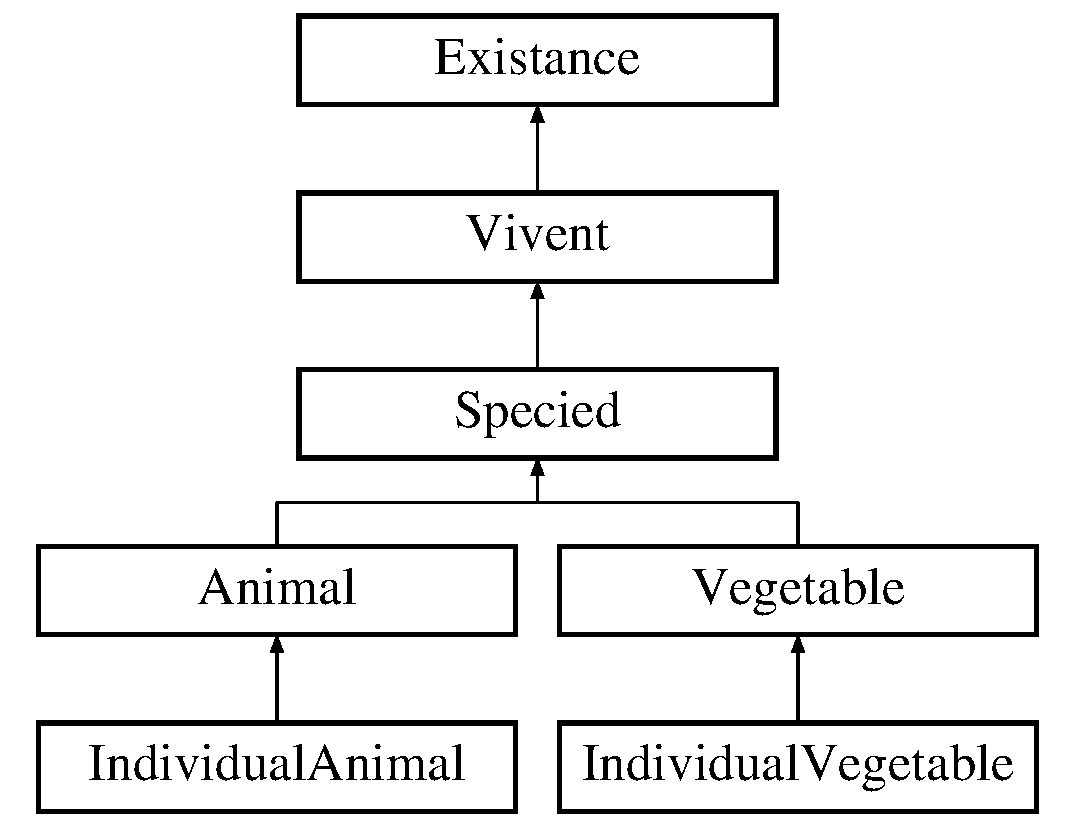
\includegraphics[height=5.000000cm]{classExistance}
\end{center}
\end{figure}
\subsection*{Public Types}
\begin{DoxyCompactItemize}
\item 
typedef long unsigned int \hyperlink{classExistance_a82c4092964457cd7da30d53072c62f1a}{id\_\-type}
\begin{DoxyCompactList}\small\item\em the type of the id\_\-number \end{DoxyCompactList}\end{DoxyCompactItemize}
\subsection*{Public Member Functions}
\begin{DoxyCompactItemize}
\item 
\hypertarget{classExistance_a415f1af7d255f9301b0a12c801404d6a}{
\hyperlink{classExistance_a415f1af7d255f9301b0a12c801404d6a}{Existance} (\hyperlink{classDateOfBirth}{DateOfBirth} u\_\-birth\_\-date=\hyperlink{classDateOfBirth}{DateOfBirth}(0, 0), \hyperlink{classExistance_a82c4092964457cd7da30d53072c62f1a}{id\_\-type} u\_\-id\_\-number=0)}
\label{classExistance_a415f1af7d255f9301b0a12c801404d6a}

\begin{DoxyCompactList}\small\item\em default constructor \end{DoxyCompactList}\item 
\hypertarget{classExistance_a38ff86bfab06fdc0b19af335b502165a}{
\hyperlink{classExistance_a38ff86bfab06fdc0b19af335b502165a}{$\sim$Existance} ()}
\label{classExistance_a38ff86bfab06fdc0b19af335b502165a}

\begin{DoxyCompactList}\small\item\em default destructor \end{DoxyCompactList}\item 
virtual bool \hyperlink{classExistance_ab86c25a779d30c45e26031e47c7b45dc}{is\_\-alive} ()=0
\begin{DoxyCompactList}\small\item\em is the existance alive? \end{DoxyCompactList}\item 
\hyperlink{classDateOfBirth}{DateOfBirth} \& \hyperlink{classExistance_a5ed0fe6062a67abff1df3ce4cae109b0}{birth\_\-date} ()
\begin{DoxyCompactList}\small\item\em the birth date \end{DoxyCompactList}\item 
\hyperlink{classExistance_a82c4092964457cd7da30d53072c62f1a}{id\_\-type} \& \hyperlink{classExistance_a23533e617509b239de916fe90811f27a}{id\_\-number} ()
\begin{DoxyCompactList}\small\item\em the id numer \end{DoxyCompactList}\item 
\hypertarget{classExistance_a1bf4ab1ba9b880175b49f914736ccd54}{
const \hyperlink{classDateOfBirth}{DateOfBirth} \& \hyperlink{classExistance_a1bf4ab1ba9b880175b49f914736ccd54}{birth\_\-date} () const }
\label{classExistance_a1bf4ab1ba9b880175b49f914736ccd54}

\begin{DoxyCompactList}\small\item\em get the birth date \end{DoxyCompactList}\item 
\hypertarget{classExistance_ad8b3c9cfa5c5be0f1420b4e43e78e227}{
\hyperlink{classExistance_a82c4092964457cd7da30d53072c62f1a}{id\_\-type} \hyperlink{classExistance_ad8b3c9cfa5c5be0f1420b4e43e78e227}{id\_\-number} () const }
\label{classExistance_ad8b3c9cfa5c5be0f1420b4e43e78e227}

\begin{DoxyCompactList}\small\item\em get the id\_\-number \end{DoxyCompactList}\end{DoxyCompactItemize}
\subsection*{Private Attributes}
\begin{DoxyCompactItemize}
\item 
\hyperlink{classDateOfBirth}{DateOfBirth} \hyperlink{classExistance_aee261695e56ed7a8d1d72aea3beb8fae}{m\_\-birth\_\-date}
\begin{DoxyCompactList}\small\item\em when an Existace is created \end{DoxyCompactList}\item 
\hyperlink{classExistance_a82c4092964457cd7da30d53072c62f1a}{id\_\-type} \hyperlink{classExistance_a6efaefb1b86cde1108adb1e71f33f84f}{m\_\-id\_\-number}
\begin{DoxyCompactList}\small\item\em unique identifier of a form of life \end{DoxyCompactList}\end{DoxyCompactItemize}


\subsection{Detailed Description}
class \hyperlink{classExistance}{Existance} the most abstracted object 

this class is the most abstract object and it's pure virtual class. all the form of life in the program eredit from her 

Definition at line 40 of file existance.h.



\subsection{Member Typedef Documentation}
\hypertarget{classExistance_a82c4092964457cd7da30d53072c62f1a}{
\index{Existance@{Existance}!id\_\-type@{id\_\-type}}
\index{id\_\-type@{id\_\-type}!Existance@{Existance}}
\subsubsection[{id\_\-type}]{\setlength{\rightskip}{0pt plus 5cm}typedef long unsigned int {\bf Existance::id\_\-type}}}
\label{classExistance_a82c4092964457cd7da30d53072c62f1a}


the type of the id\_\-number 

long unsigned int 

Definition at line 46 of file existance.h.



\subsection{Member Function Documentation}
\hypertarget{classExistance_a5ed0fe6062a67abff1df3ce4cae109b0}{
\index{Existance@{Existance}!birth\_\-date@{birth\_\-date}}
\index{birth\_\-date@{birth\_\-date}!Existance@{Existance}}
\subsubsection[{birth\_\-date}]{\setlength{\rightskip}{0pt plus 5cm}{\bf DateOfBirth} \& Existance::birth\_\-date (
\begin{DoxyParamCaption}
{}
\end{DoxyParamCaption}
)}}
\label{classExistance_a5ed0fe6062a67abff1df3ce4cae109b0}


the birth date 

da birth date \begin{DoxySeeAlso}{See also}
\hyperlink{classDateOfBirth}{DateOfBirth} 

\hyperlink{classExistance_aee261695e56ed7a8d1d72aea3beb8fae}{m\_\-birth\_\-date} 
\end{DoxySeeAlso}


Definition at line 48 of file existance.cpp.

\hypertarget{classExistance_a23533e617509b239de916fe90811f27a}{
\index{Existance@{Existance}!id\_\-number@{id\_\-number}}
\index{id\_\-number@{id\_\-number}!Existance@{Existance}}
\subsubsection[{id\_\-number}]{\setlength{\rightskip}{0pt plus 5cm}{\bf Existance::id\_\-type} \& Existance::id\_\-number (
\begin{DoxyParamCaption}
{}
\end{DoxyParamCaption}
)}}
\label{classExistance_a23533e617509b239de916fe90811f27a}


the id numer 

\begin{DoxySeeAlso}{See also}
\hyperlink{classExistance_a6efaefb1b86cde1108adb1e71f33f84f}{m\_\-id\_\-number} 
\end{DoxySeeAlso}


Definition at line 53 of file existance.cpp.

\hypertarget{classExistance_ab86c25a779d30c45e26031e47c7b45dc}{
\index{Existance@{Existance}!is\_\-alive@{is\_\-alive}}
\index{is\_\-alive@{is\_\-alive}!Existance@{Existance}}
\subsubsection[{is\_\-alive}]{\setlength{\rightskip}{0pt plus 5cm}virtual bool Existance::is\_\-alive (
\begin{DoxyParamCaption}
{}
\end{DoxyParamCaption}
)\hspace{0.3cm}{\ttfamily  \mbox{[}pure virtual\mbox{]}}}}
\label{classExistance_ab86c25a779d30c45e26031e47c7b45dc}


is the existance alive? 

returns true if the object is alive. existance cannot be whithout their specifications, so this member is pure virtual 

Implemented in \hyperlink{classIndividualAnimal_a78960ddab5b3649638ba6b97238edc06}{IndividualAnimal}, \hyperlink{classSpecied_a2173ab978d5cd2c2de4e25a4d6eb3152}{Specied}, and \hyperlink{classVivent_a253291090ae6207f8f51f8ff669d9d17}{Vivent}.



\subsection{Member Data Documentation}
\hypertarget{classExistance_aee261695e56ed7a8d1d72aea3beb8fae}{
\index{Existance@{Existance}!m\_\-birth\_\-date@{m\_\-birth\_\-date}}
\index{m\_\-birth\_\-date@{m\_\-birth\_\-date}!Existance@{Existance}}
\subsubsection[{m\_\-birth\_\-date}]{\setlength{\rightskip}{0pt plus 5cm}{\bf DateOfBirth} {\bf Existance::m\_\-birth\_\-date}\hspace{0.3cm}{\ttfamily  \mbox{[}private\mbox{]}}}}
\label{classExistance_aee261695e56ed7a8d1d72aea3beb8fae}


when an Existace is created 

every form of life has a date of birth. see \hyperlink{classDateOfBirth}{DateOfBirth} for more info. \begin{DoxySeeAlso}{See also}
\hyperlink{classDateOfBirth}{DateOfBirth} 
\end{DoxySeeAlso}


Definition at line 88 of file existance.h.

\hypertarget{classExistance_a6efaefb1b86cde1108adb1e71f33f84f}{
\index{Existance@{Existance}!m\_\-id\_\-number@{m\_\-id\_\-number}}
\index{m\_\-id\_\-number@{m\_\-id\_\-number}!Existance@{Existance}}
\subsubsection[{m\_\-id\_\-number}]{\setlength{\rightskip}{0pt plus 5cm}{\bf id\_\-type} {\bf Existance::m\_\-id\_\-number}\hspace{0.3cm}{\ttfamily  \mbox{[}private\mbox{]}}}}
\label{classExistance_a6efaefb1b86cde1108adb1e71f33f84f}


unique identifier of a form of life 

this data member is different between all the form of life istanced. this property has to be granted by the gestion algorithm 

Definition at line 96 of file existance.h.



The documentation for this class was generated from the following files:\begin{DoxyCompactItemize}
\item 
sources/\hyperlink{existance_8h}{existance.h}\item 
sources/\hyperlink{existance_8cpp}{existance.cpp}\end{DoxyCompactItemize}

\hypertarget{classGender}{
\section{Gender Class Reference}
\label{classGender}\index{Gender@{Gender}}
}


the gender of the form of life  




{\ttfamily \#include $<$gender.h$>$}

\subsection*{Public Member Functions}
\begin{DoxyCompactItemize}
\item 
\hyperlink{classGender_a90e371a0a09819d60c2452238988262f}{Gender} ()
\begin{DoxyCompactList}\small\item\em default constructor \end{DoxyCompactList}\item 
\hyperlink{classGender_a359546875d33cef5599e85e58c15d8e0}{Gender} (std::string r\_\-gender)
\begin{DoxyCompactList}\small\item\em constructor using a string \end{DoxyCompactList}\item 
\hypertarget{classGender_a7ad7a7514711926743c9117dcbdefe04}{
\hyperlink{classGender_a7ad7a7514711926743c9117dcbdefe04}{$\sim$Gender} ()}
\label{classGender_a7ad7a7514711926743c9117dcbdefe04}

\begin{DoxyCompactList}\small\item\em default destructor \end{DoxyCompactList}\item 
\hypertarget{classGender_ac2ea0b219f63dddd3c8ec4511d942e38}{
bool \hyperlink{classGender_ac2ea0b219f63dddd3c8ec4511d942e38}{is\_\-male} ()}
\label{classGender_ac2ea0b219f63dddd3c8ec4511d942e38}

\begin{DoxyCompactList}\small\item\em returns true if it is male \end{DoxyCompactList}\item 
\hypertarget{classGender_a7618eefc206851181be4ac406482189e}{
bool \hyperlink{classGender_a7618eefc206851181be4ac406482189e}{is\_\-female} ()}
\label{classGender_a7618eefc206851181be4ac406482189e}

\begin{DoxyCompactList}\small\item\em returns true if it is female \end{DoxyCompactList}\item 
\hypertarget{classGender_a5be5137cbbe3177d3934b78f23c19e87}{
bool \hyperlink{classGender_a5be5137cbbe3177d3934b78f23c19e87}{is\_\-hermaphrodite} ()}
\label{classGender_a5be5137cbbe3177d3934b78f23c19e87}

\begin{DoxyCompactList}\small\item\em returns true if it is hermaphrodite \end{DoxyCompactList}\item 
\hypertarget{classGender_ad1e9c77e0075959e59995ae5f0587695}{
bool \hyperlink{classGender_ad1e9c77e0075959e59995ae5f0587695}{is\_\-asexual} ()}
\label{classGender_ad1e9c77e0075959e59995ae5f0587695}

\begin{DoxyCompactList}\small\item\em returns true if it is asexual \end{DoxyCompactList}\item 
\hypertarget{classGender_a454a9f9b3605d4df6ad3125fbcb78dd2}{
const std::string \& \hyperlink{classGender_a454a9f9b3605d4df6ad3125fbcb78dd2}{gender} () const }
\label{classGender_a454a9f9b3605d4df6ad3125fbcb78dd2}

\begin{DoxyCompactList}\small\item\em get gender name \end{DoxyCompactList}\item 
void \hyperlink{classGender_a931859ed381f2adb1a5aa54f163db24c}{change\_\-gender} (std::string r\_\-gender)
\begin{DoxyCompactList}\small\item\em change the sex \end{DoxyCompactList}\item 
void \hyperlink{classGender_a74e44c24c4c8748aa9aa2a884a03e2a3}{change\_\-gender} (const unsigned int u\_\-gender\_\-num=4)
\begin{DoxyCompactList}\small\item\em change the sex \end{DoxyCompactList}\item 
unsigned int \hyperlink{classGender_ab1e46219176ba4a6b63fa3e0ce45d3b7}{numerical\_\-gender} () const 
\begin{DoxyCompactList}\small\item\em numerical gender \end{DoxyCompactList}\item 
\hypertarget{classGender_a9c20ed5c2c47837c2fce7686d42e0325}{
bool \hyperlink{classGender_a9c20ed5c2c47837c2fce7686d42e0325}{operator$<$} (const \hyperlink{classGender}{Gender} \&gen) const }
\label{classGender_a9c20ed5c2c47837c2fce7686d42e0325}

\begin{DoxyCompactList}\small\item\em operator $<$ \end{DoxyCompactList}\end{DoxyCompactItemize}
\subsection*{Private Attributes}
\begin{DoxyCompactItemize}
\item 
\hypertarget{classGender_a57094c4220de22c3f5d2f0876a28695a}{
bool \hyperlink{classGender_a57094c4220de22c3f5d2f0876a28695a}{male\_\-}}
\label{classGender_a57094c4220de22c3f5d2f0876a28695a}

\begin{DoxyCompactList}\small\item\em if true is a male \end{DoxyCompactList}\item 
\hypertarget{classGender_a1f13af5f143d7a202fcf1e406595071f}{
bool \hyperlink{classGender_a1f13af5f143d7a202fcf1e406595071f}{female\_\-}}
\label{classGender_a1f13af5f143d7a202fcf1e406595071f}

\begin{DoxyCompactList}\small\item\em if true is a female \end{DoxyCompactList}\item 
\hypertarget{classGender_a9c64708993b555550d8effa0f5da74c1}{
std::string \hyperlink{classGender_a9c64708993b555550d8effa0f5da74c1}{gender\_\-name\_\-}}
\label{classGender_a9c64708993b555550d8effa0f5da74c1}

\begin{DoxyCompactList}\small\item\em name of the gender \end{DoxyCompactList}\end{DoxyCompactItemize}
\subsection*{Friends}
\begin{DoxyCompactItemize}
\item 
std::ostream \& \hyperlink{classGender_a880decf4751cb0cf4d7b30cfa096a758}{operator$<$$<$} (std::ostream \&os, const \hyperlink{classGender}{Gender} \&gen)
\begin{DoxyCompactList}\small\item\em ostream operator of gender \end{DoxyCompactList}\end{DoxyCompactItemize}


\subsection{Detailed Description}
the gender of the form of life 

the possible gender of a form of life where: male , female, ermaphrodite, asexual;

this is decided by the values of male\_\- and female\_\-;

the ermaphrodite is male and female at the same time, the asexual is nor male nor female.

\begin{DoxySeeAlso}{See also}
\hyperlink{classGender_a57094c4220de22c3f5d2f0876a28695a}{male\_\-} 

\hyperlink{classGender_a1f13af5f143d7a202fcf1e406595071f}{female\_\-} 
\end{DoxySeeAlso}


Definition at line 48 of file gender.h.



\subsection{Constructor \& Destructor Documentation}
\hypertarget{classGender_a90e371a0a09819d60c2452238988262f}{
\index{Gender@{Gender}!Gender@{Gender}}
\index{Gender@{Gender}!Gender@{Gender}}
\subsubsection[{Gender}]{\setlength{\rightskip}{0pt plus 5cm}Gender::Gender (
\begin{DoxyParamCaption}
{}
\end{DoxyParamCaption}
)}}
\label{classGender_a90e371a0a09819d60c2452238988262f}


default constructor 

if no argument were given the form of life is considered asexual 

Definition at line 32 of file gender.cpp.

\hypertarget{classGender_a359546875d33cef5599e85e58c15d8e0}{
\index{Gender@{Gender}!Gender@{Gender}}
\index{Gender@{Gender}!Gender@{Gender}}
\subsubsection[{Gender}]{\setlength{\rightskip}{0pt plus 5cm}Gender::Gender (
\begin{DoxyParamCaption}
\item[{std::string}]{r\_\-gender}
\end{DoxyParamCaption}
)}}
\label{classGender_a359546875d33cef5599e85e58c15d8e0}


constructor using a string 


\begin{DoxyParams}{Parameters}
{\em r\_\-gender} & is the string containing the gender specification given in runtime. possible values are: \char`\"{}male\char`\"{} , \char`\"{}female\char`\"{} , \char`\"{}ermaphrodite\char`\"{} , \char`\"{}asexual\char`\"{};\\
\hline
\end{DoxyParams}
if the gender is speciefied badly the gender is set to asexual; 

Definition at line 42 of file gender.cpp.



\subsection{Member Function Documentation}
\hypertarget{classGender_a931859ed381f2adb1a5aa54f163db24c}{
\index{Gender@{Gender}!change\_\-gender@{change\_\-gender}}
\index{change\_\-gender@{change\_\-gender}!Gender@{Gender}}
\subsubsection[{change\_\-gender}]{\setlength{\rightskip}{0pt plus 5cm}void Gender::change\_\-gender (
\begin{DoxyParamCaption}
\item[{std::string}]{r\_\-gender}
\end{DoxyParamCaption}
)}}
\label{classGender_a931859ed381f2adb1a5aa54f163db24c}


change the sex 

need a string like the constructos 
\begin{DoxyParams}{Parameters}
{\em r\_\-gender} & see \hyperlink{classGender_a90e371a0a09819d60c2452238988262f}{Gender()} \\
\hline
\end{DoxyParams}


Definition at line 110 of file gender.cpp.

\hypertarget{classGender_a74e44c24c4c8748aa9aa2a884a03e2a3}{
\index{Gender@{Gender}!change\_\-gender@{change\_\-gender}}
\index{change\_\-gender@{change\_\-gender}!Gender@{Gender}}
\subsubsection[{change\_\-gender}]{\setlength{\rightskip}{0pt plus 5cm}void Gender::change\_\-gender (
\begin{DoxyParamCaption}
\item[{const unsigned int}]{u\_\-gender\_\-num = {\ttfamily 4}}
\end{DoxyParamCaption}
)}}
\label{classGender_a74e44c24c4c8748aa9aa2a884a03e2a3}


change the sex 


\begin{DoxyParams}{Parameters}
{\em u\_\-gender\_\-num} & see numerical\_\-gender \\
\hline
\end{DoxyParams}


Definition at line 152 of file gender.cpp.

\hypertarget{classGender_ab1e46219176ba4a6b63fa3e0ce45d3b7}{
\index{Gender@{Gender}!numerical\_\-gender@{numerical\_\-gender}}
\index{numerical\_\-gender@{numerical\_\-gender}!Gender@{Gender}}
\subsubsection[{numerical\_\-gender}]{\setlength{\rightskip}{0pt plus 5cm}unsigned int Gender::numerical\_\-gender (
\begin{DoxyParamCaption}
{}
\end{DoxyParamCaption}
) const}}
\label{classGender_ab1e46219176ba4a6b63fa3e0ce45d3b7}


numerical gender 

return a numerical id (int) which rappresent the gender. 1 is male, 2 is female, 3 is hermaphrodite and 4 is asexual; 

Definition at line 195 of file gender.cpp.



\subsection{Friends And Related Function Documentation}
\hypertarget{classGender_a880decf4751cb0cf4d7b30cfa096a758}{
\index{Gender@{Gender}!operator$<$$<$@{operator$<$$<$}}
\index{operator$<$$<$@{operator$<$$<$}!Gender@{Gender}}
\subsubsection[{operator$<$$<$}]{\setlength{\rightskip}{0pt plus 5cm}std::ostream\& operator$<$$<$ (
\begin{DoxyParamCaption}
\item[{std::ostream \&}]{os, }
\item[{const {\bf Gender} \&}]{gen}
\end{DoxyParamCaption}
)\hspace{0.3cm}{\ttfamily  \mbox{[}friend\mbox{]}}}}
\label{classGender_a880decf4751cb0cf4d7b30cfa096a758}


ostream operator of gender 

prints a string saying the actual gender is a wrapper of \hyperlink{classGender_a454a9f9b3605d4df6ad3125fbcb78dd2}{Gender::gender()} 

Definition at line 213 of file gender.cpp.



The documentation for this class was generated from the following files:\begin{DoxyCompactItemize}
\item 
sources/\hyperlink{gender_8h}{gender.h}\item 
sources/\hyperlink{gender_8cpp}{gender.cpp}\end{DoxyCompactItemize}

\hypertarget{classGrafico}{
\section{Grafico Class Reference}
\label{classGrafico}\index{Grafico@{Grafico}}
}
\subsection*{Public Member Functions}
\begin{DoxyCompactItemize}
\item 
\hypertarget{classGrafico_aadf0c06b1014d6dc134c8c49a582316e}{
{\bfseries Grafico} (string)}
\label{classGrafico_aadf0c06b1014d6dc134c8c49a582316e}

\item 
\hypertarget{classGrafico_a8e6649a1af93b702263b994b21dbc462}{
void {\bfseries Set\_\-title} (string)}
\label{classGrafico_a8e6649a1af93b702263b994b21dbc462}

\item 
\hypertarget{classGrafico_ac826d42294c1a312d74da3333dc8e5dc}{
void {\bfseries Set\_\-xlabel} (string)}
\label{classGrafico_ac826d42294c1a312d74da3333dc8e5dc}

\item 
\hypertarget{classGrafico_af2bfef0c397a17708240262d0461fcb6}{
void {\bfseries Set\_\-ylabel} (string)}
\label{classGrafico_af2bfef0c397a17708240262d0461fcb6}

\item 
\hypertarget{classGrafico_ab0e092d9bebb8edd6f0c2dcdab2cf06f}{
void {\bfseries Set\_\-labels} (string, string)}
\label{classGrafico_ab0e092d9bebb8edd6f0c2dcdab2cf06f}

\item 
\hypertarget{classGrafico_a8cb74b0876afde61846069754544073b}{
void {\bfseries Set\_\-xrange} (double, double)}
\label{classGrafico_a8cb74b0876afde61846069754544073b}

\item 
\hypertarget{classGrafico_a32f216386dea3383cc05338e901f72ce}{
void {\bfseries Set\_\-yrange} (double, double)}
\label{classGrafico_a32f216386dea3383cc05338e901f72ce}

\item 
\hypertarget{classGrafico_a444a3b0ae461aee9b4ef014147386c07}{
void {\bfseries Add\_\-grafico} (double $\ast$, double $\ast$, int, string)}
\label{classGrafico_a444a3b0ae461aee9b4ef014147386c07}

\item 
\hypertarget{classGrafico_aae244e1e2f84a14f3981c360f72108fc}{
void {\bfseries Set\_\-data\_\-style} (string)}
\label{classGrafico_aae244e1e2f84a14f3981c360f72108fc}

\item 
\hypertarget{classGrafico_a5f3691106d812f2fea2e7d379078bfb4}{
void {\bfseries Legend\_\-position} (int)}
\label{classGrafico_a5f3691106d812f2fea2e7d379078bfb4}

\end{DoxyCompactItemize}
\subsection*{Private Attributes}
\begin{DoxyCompactItemize}
\item 
\hypertarget{classGrafico_a92d61d84ee22b7baa82aa755a7dece87}{
fstream {\bfseries \_\-comandi}}
\label{classGrafico_a92d61d84ee22b7baa82aa755a7dece87}

\item 
\hypertarget{classGrafico_aaec41fc74fff525a7ecbc4e0d3971cc5}{
char $\ast$ {\bfseries \_\-file}}
\label{classGrafico_aaec41fc74fff525a7ecbc4e0d3971cc5}

\item 
\hypertarget{classGrafico_aa051b59955412fea00373b3af09d2fc6}{
int {\bfseries \_\-N\_\-grafici}}
\label{classGrafico_aa051b59955412fea00373b3af09d2fc6}

\item 
\hypertarget{classGrafico_a31add51cf1e043c1fd44eb116f4c7ed1}{
string {\bfseries \_\-immagine}}
\label{classGrafico_a31add51cf1e043c1fd44eb116f4c7ed1}

\end{DoxyCompactItemize}


\subsection{Detailed Description}


Definition at line 34 of file grafico.hpp.



The documentation for this class was generated from the following files:\begin{DoxyCompactItemize}
\item 
sources/grafico.hpp\item 
sources/grafico.cpp\end{DoxyCompactItemize}

\hypertarget{structSubsystemContainer_1_1id}{
\section{SubsystemContainer::id Struct Reference}
\label{structSubsystemContainer_1_1id}\index{SubsystemContainer::id@{SubsystemContainer::id}}
}


boost multyindex::ordered\_\-index tag  




{\ttfamily \#include $<$subsystemcontainer.h$>$}



\subsection{Detailed Description}
boost multyindex::ordered\_\-index tag 

Definition at line 81 of file subsystemcontainer.h.



The documentation for this struct was generated from the following file:\begin{DoxyCompactItemize}
\item 
sources/\hyperlink{subsystemcontainer_8h}{subsystemcontainer.h}\end{DoxyCompactItemize}

\hypertarget{classIndividualAnimal}{
\section{IndividualAnimal Class Reference}
\label{classIndividualAnimal}\index{IndividualAnimal@{IndividualAnimal}}
}


class \hyperlink{classIndividualAnimal}{IndividualAnimal}  




{\ttfamily \#include $<$individualanimal.h$>$}

Inheritance diagram for IndividualAnimal:\begin{figure}[H]
\begin{center}
\leavevmode
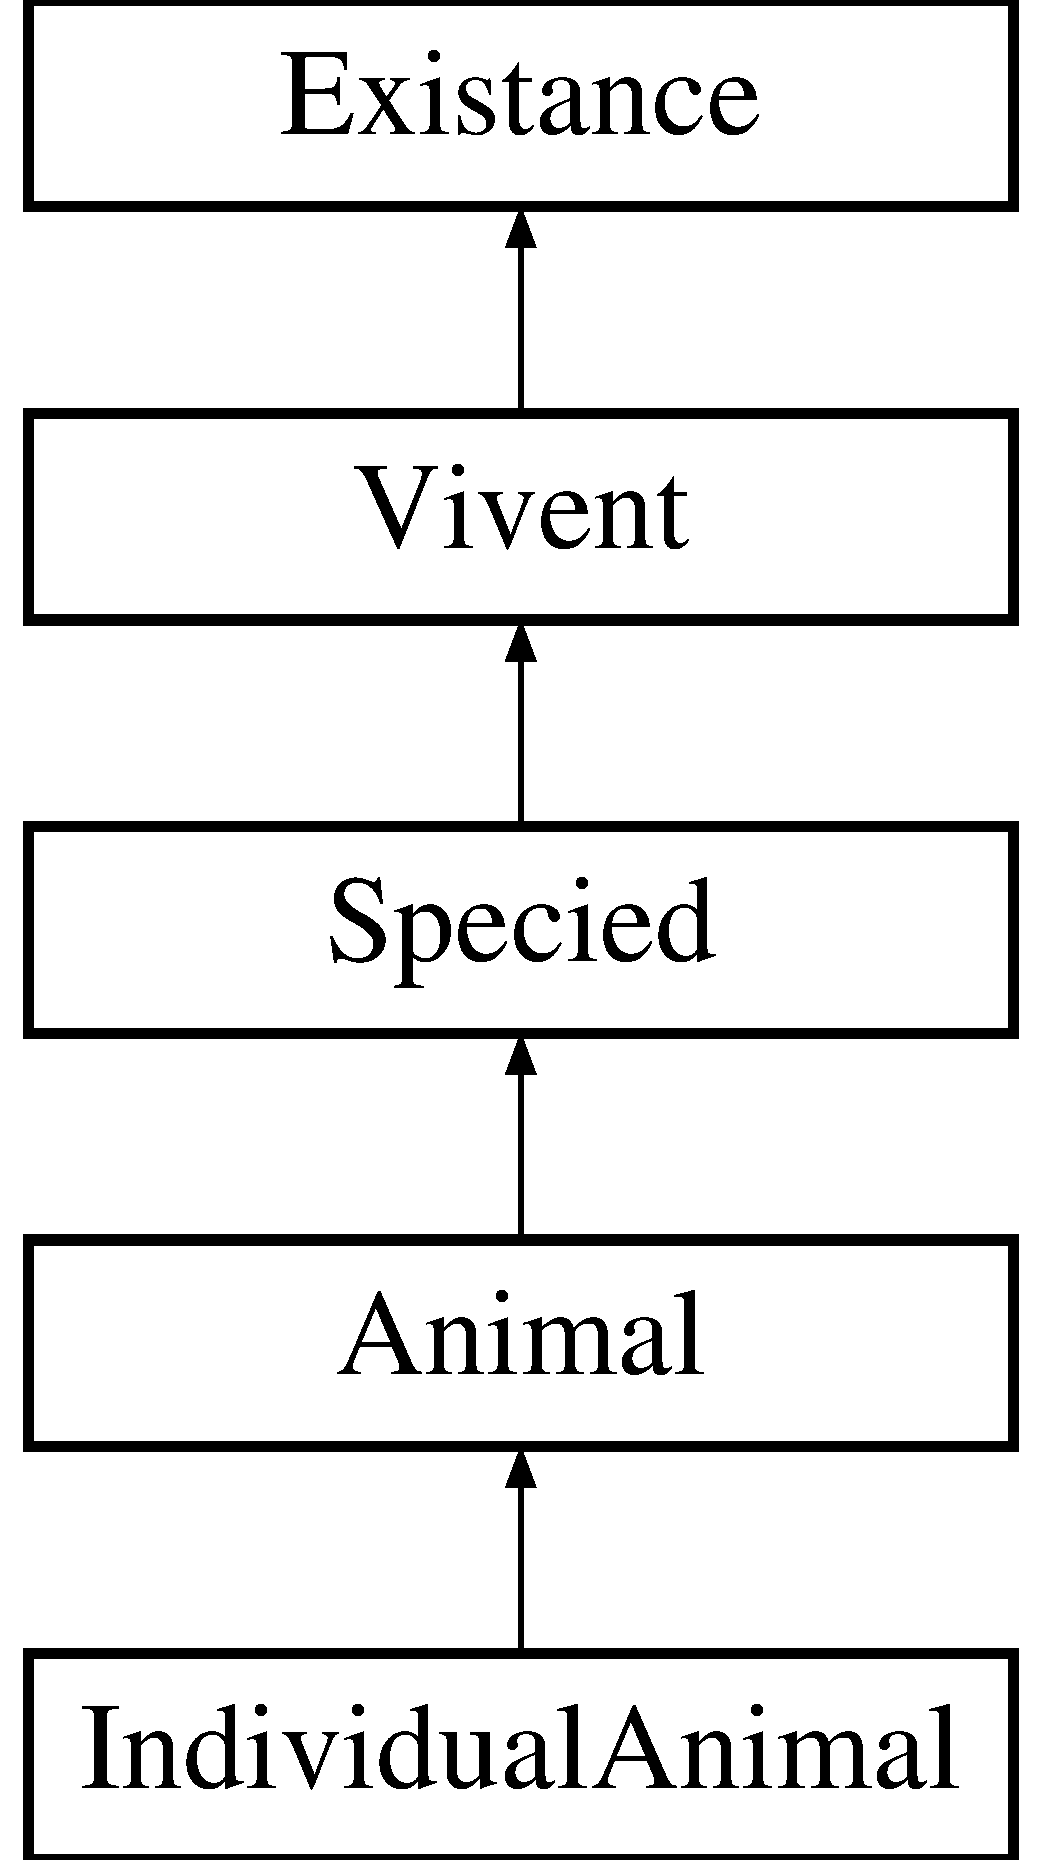
\includegraphics[height=5.000000cm]{classIndividualAnimal}
\end{center}
\end{figure}
\subsection*{Public Member Functions}
\begin{DoxyCompactItemize}
\item 
\hyperlink{classIndividualAnimal_a44ab68443a3df25e11ec525a42782d43}{IndividualAnimal} (unsigned int u\_\-appetite=0, unsigned int u\_\-libido=0)
\begin{DoxyCompactList}\small\item\em default constructor \end{DoxyCompactList}\item 
\hyperlink{classIndividualAnimal_a145f082f37b866b1b36c4efd44e06900}{$\sim$IndividualAnimal} ()
\begin{DoxyCompactList}\small\item\em default destructor \end{DoxyCompactList}\item 
\hypertarget{classIndividualAnimal_a78960ddab5b3649638ba6b97238edc06}{
virtual bool \hyperlink{classIndividualAnimal_a78960ddab5b3649638ba6b97238edc06}{is\_\-alive} ()}
\label{classIndividualAnimal_a78960ddab5b3649638ba6b97238edc06}

\begin{DoxyCompactList}\small\item\em compute id the animal is alive \end{DoxyCompactList}\item 
\hypertarget{classIndividualAnimal_adedd04efd80eea6cb721e830c545fe54}{
unsigned int \& \hyperlink{classIndividualAnimal_adedd04efd80eea6cb721e830c545fe54}{appetite} ()}
\label{classIndividualAnimal_adedd04efd80eea6cb721e830c545fe54}

\begin{DoxyCompactList}\small\item\em set appetite \end{DoxyCompactList}\item 
\hypertarget{classIndividualAnimal_a128b28bad2036c848c0d7525d366c7da}{
unsigned int \& \hyperlink{classIndividualAnimal_a128b28bad2036c848c0d7525d366c7da}{libido} ()}
\label{classIndividualAnimal_a128b28bad2036c848c0d7525d366c7da}

\begin{DoxyCompactList}\small\item\em set libido \end{DoxyCompactList}\item 
\hypertarget{classIndividualAnimal_a38f21a847bdd5c01c782ea0192f27c57}{
unsigned int \hyperlink{classIndividualAnimal_a38f21a847bdd5c01c782ea0192f27c57}{appetite} () const }
\label{classIndividualAnimal_a38f21a847bdd5c01c782ea0192f27c57}

\begin{DoxyCompactList}\small\item\em get appetite \end{DoxyCompactList}\item 
\hypertarget{classIndividualAnimal_ac245ea10d23617781d639622bd65d75d}{
unsigned int \hyperlink{classIndividualAnimal_ac245ea10d23617781d639622bd65d75d}{libido} () const }
\label{classIndividualAnimal_ac245ea10d23617781d639622bd65d75d}

\begin{DoxyCompactList}\small\item\em get libido \end{DoxyCompactList}\end{DoxyCompactItemize}
\subsection*{Private Attributes}
\begin{DoxyCompactItemize}
\item 
unsigned int \hyperlink{classIndividualAnimal_a1ffbeb4d91923e91679c96f1e45e5071}{m\_\-appetite}
\begin{DoxyCompactList}\small\item\em appetite factor \end{DoxyCompactList}\item 
unsigned int \hyperlink{classIndividualAnimal_a60d160394b92b61685a63f3c91164938}{m\_\-libido}
\begin{DoxyCompactList}\small\item\em libido factor \end{DoxyCompactList}\end{DoxyCompactItemize}
\subsection*{Friends}
\begin{DoxyCompactItemize}
\item 
std::ostream \& \hyperlink{classIndividualAnimal_abaf2e3cb53c5c0004f0fa218ab980965}{operator$<$$<$} (std::ostream \&os, const \hyperlink{classIndividualAnimal}{IndividualAnimal} \&an)
\begin{DoxyCompactList}\small\item\em ostream operator \end{DoxyCompactList}\end{DoxyCompactItemize}


\subsection{Detailed Description}
class \hyperlink{classIndividualAnimal}{IndividualAnimal} 

this class rappresent the animal see as the final and real living form of life. each animal differs from the other by his appetite and his libido 

Definition at line 39 of file individualanimal.h.



\subsection{Constructor \& Destructor Documentation}
\hypertarget{classIndividualAnimal_a44ab68443a3df25e11ec525a42782d43}{
\index{IndividualAnimal@{IndividualAnimal}!IndividualAnimal@{IndividualAnimal}}
\index{IndividualAnimal@{IndividualAnimal}!IndividualAnimal@{IndividualAnimal}}
\subsubsection[{IndividualAnimal}]{\setlength{\rightskip}{0pt plus 5cm}IndividualAnimal::IndividualAnimal (
\begin{DoxyParamCaption}
\item[{unsigned int}]{u\_\-appetite = {\ttfamily 0}, }
\item[{unsigned int}]{u\_\-libido = {\ttfamily 0}}
\end{DoxyParamCaption}
)}}
\label{classIndividualAnimal_a44ab68443a3df25e11ec525a42782d43}


default constructor 

set appetite and libido, if none were given they were setted to 0 both. 

Definition at line 37 of file individualanimal.cpp.

\hypertarget{classIndividualAnimal_a145f082f37b866b1b36c4efd44e06900}{
\index{IndividualAnimal@{IndividualAnimal}!$\sim$IndividualAnimal@{$\sim$IndividualAnimal}}
\index{$\sim$IndividualAnimal@{$\sim$IndividualAnimal}!IndividualAnimal@{IndividualAnimal}}
\subsubsection[{$\sim$IndividualAnimal}]{\setlength{\rightskip}{0pt plus 5cm}IndividualAnimal::$\sim$IndividualAnimal (
\begin{DoxyParamCaption}
{}
\end{DoxyParamCaption}
)}}
\label{classIndividualAnimal_a145f082f37b866b1b36c4efd44e06900}


default destructor 

does nothing 

Definition at line 44 of file individualanimal.cpp.



\subsection{Friends And Related Function Documentation}
\hypertarget{classIndividualAnimal_abaf2e3cb53c5c0004f0fa218ab980965}{
\index{IndividualAnimal@{IndividualAnimal}!operator$<$$<$@{operator$<$$<$}}
\index{operator$<$$<$@{operator$<$$<$}!IndividualAnimal@{IndividualAnimal}}
\subsubsection[{operator$<$$<$}]{\setlength{\rightskip}{0pt plus 5cm}std::ostream\& operator$<$$<$ (
\begin{DoxyParamCaption}
\item[{std::ostream \&}]{os, }
\item[{const {\bf IndividualAnimal} \&}]{an}
\end{DoxyParamCaption}
)\hspace{0.3cm}{\ttfamily  \mbox{[}friend\mbox{]}}}}
\label{classIndividualAnimal_abaf2e3cb53c5c0004f0fa218ab980965}


ostream operator 

prints al main info of the animal 

Definition at line 76 of file individualanimal.cpp.



\subsection{Member Data Documentation}
\hypertarget{classIndividualAnimal_a1ffbeb4d91923e91679c96f1e45e5071}{
\index{IndividualAnimal@{IndividualAnimal}!m\_\-appetite@{m\_\-appetite}}
\index{m\_\-appetite@{m\_\-appetite}!IndividualAnimal@{IndividualAnimal}}
\subsubsection[{m\_\-appetite}]{\setlength{\rightskip}{0pt plus 5cm}unsigned int {\bf IndividualAnimal::m\_\-appetite}\hspace{0.3cm}{\ttfamily  \mbox{[}private\mbox{]}}}}
\label{classIndividualAnimal_a1ffbeb4d91923e91679c96f1e45e5071}


appetite factor 

it rappresents the propensity of the animal to eat and rise when the hp of the animal were under the health status

\begin{DoxySeeAlso}{See also}
\hyperlink{classSpecied_a7d716a70352c40bbe1ff3bd8c5719f29}{m\_\-health\_\-status} 
\end{DoxySeeAlso}


Definition at line 85 of file individualanimal.h.

\hypertarget{classIndividualAnimal_a60d160394b92b61685a63f3c91164938}{
\index{IndividualAnimal@{IndividualAnimal}!m\_\-libido@{m\_\-libido}}
\index{m\_\-libido@{m\_\-libido}!IndividualAnimal@{IndividualAnimal}}
\subsubsection[{m\_\-libido}]{\setlength{\rightskip}{0pt plus 5cm}unsigned int {\bf IndividualAnimal::m\_\-libido}\hspace{0.3cm}{\ttfamily  \mbox{[}private\mbox{]}}}}
\label{classIndividualAnimal_a60d160394b92b61685a63f3c91164938}


libido factor 

pay attention: parental controll pending. btw the libido factor determines the propensity of the animal to reproduce and rises when the animal's hp where under the health status \begin{DoxySeeAlso}{See also}
\hyperlink{classSpecied_a7d716a70352c40bbe1ff3bd8c5719f29}{m\_\-health\_\-status} 
\end{DoxySeeAlso}


Definition at line 93 of file individualanimal.h.



The documentation for this class was generated from the following files:\begin{DoxyCompactItemize}
\item 
sources/\hyperlink{individualanimal_8h}{individualanimal.h}\item 
sources/\hyperlink{individualanimal_8cpp}{individualanimal.cpp}\end{DoxyCompactItemize}

\hypertarget{classIndividualVegetable}{
\section{IndividualVegetable Class Reference}
\label{classIndividualVegetable}\index{IndividualVegetable@{IndividualVegetable}}
}


class \hyperlink{classIndividualVegetable}{IndividualVegetable}  




{\ttfamily \#include $<$individualvegetable.h$>$}

Inheritance diagram for IndividualVegetable:\begin{figure}[H]
\begin{center}
\leavevmode
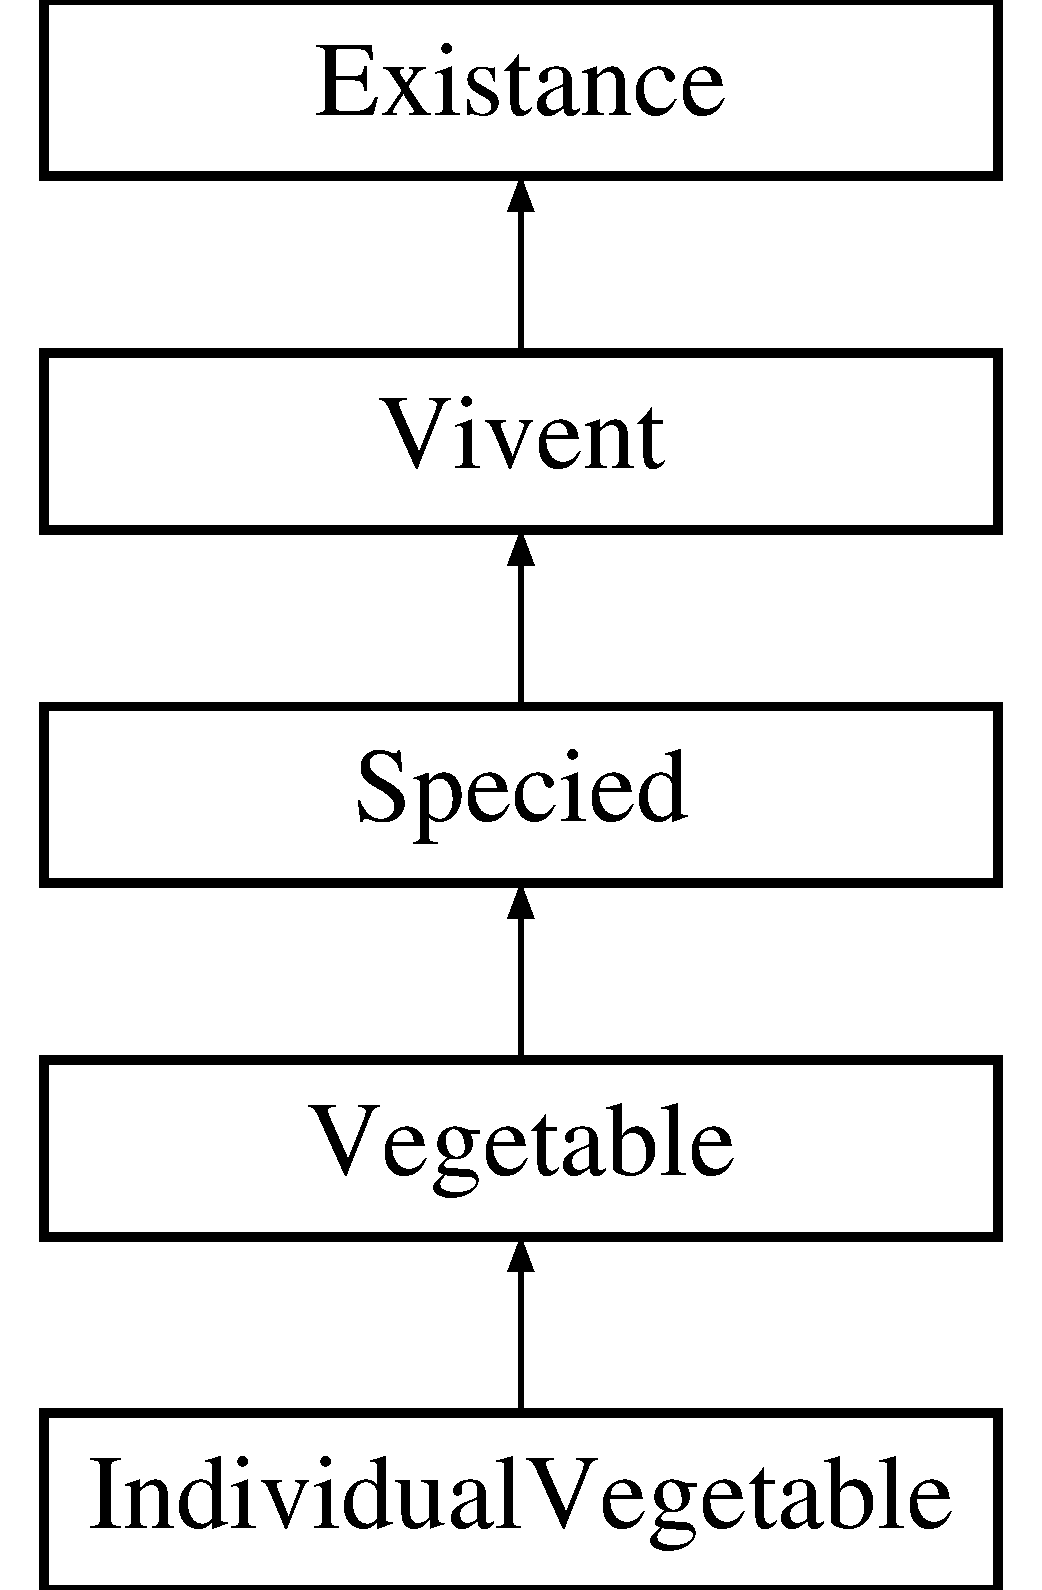
\includegraphics[height=5.000000cm]{classIndividualVegetable}
\end{center}
\end{figure}
\subsection*{Public Member Functions}
\begin{DoxyCompactItemize}
\item 
\hypertarget{classIndividualVegetable_a4c6d823618f7f9569b465d58a0fbf6be}{
\hyperlink{classIndividualVegetable_a4c6d823618f7f9569b465d58a0fbf6be}{IndividualVegetable} ()}
\label{classIndividualVegetable_a4c6d823618f7f9569b465d58a0fbf6be}

\begin{DoxyCompactList}\small\item\em default contructor \end{DoxyCompactList}\item 
\hypertarget{classIndividualVegetable_a6015588a2374d86b69a85bb269b3b2de}{
\hyperlink{classIndividualVegetable_a6015588a2374d86b69a85bb269b3b2de}{$\sim$IndividualVegetable} ()}
\label{classIndividualVegetable_a6015588a2374d86b69a85bb269b3b2de}

\begin{DoxyCompactList}\small\item\em default destructor \end{DoxyCompactList}\end{DoxyCompactItemize}
\subsection*{Friends}
\begin{DoxyCompactItemize}
\item 
std::ostream \& \hyperlink{classIndividualVegetable_abf637bb4de2994493dfe49c0bba1ce80}{operator$<$$<$} (std::ostream \&os, const \hyperlink{classIndividualVegetable}{IndividualVegetable} \&veg)
\begin{DoxyCompactList}\small\item\em prints the individual vegetable \end{DoxyCompactList}\end{DoxyCompactItemize}


\subsection{Detailed Description}
class \hyperlink{classIndividualVegetable}{IndividualVegetable} 

class rappresenting the vegetable seen as a single form of life. for this implementation no more features are added in order to differentiate \hyperlink{classIndividualVegetable}{IndividualVegetable} to \hyperlink{classSpecied}{Specied}. by the way this had been done to give the future possibiliti to implement vegetable reproduction or feeding. 

Definition at line 40 of file individualvegetable.h.



\subsection{Friends And Related Function Documentation}
\hypertarget{classIndividualVegetable_abf637bb4de2994493dfe49c0bba1ce80}{
\index{IndividualVegetable@{IndividualVegetable}!operator$<$$<$@{operator$<$$<$}}
\index{operator$<$$<$@{operator$<$$<$}!IndividualVegetable@{IndividualVegetable}}
\subsubsection[{operator$<$$<$}]{\setlength{\rightskip}{0pt plus 5cm}std::ostream\& operator$<$$<$ (
\begin{DoxyParamCaption}
\item[{std::ostream \&}]{os, }
\item[{const {\bf IndividualVegetable} \&}]{veg}
\end{DoxyParamCaption}
)\hspace{0.3cm}{\ttfamily  \mbox{[}friend\mbox{]}}}}
\label{classIndividualVegetable_abf637bb4de2994493dfe49c0bba1ce80}


prints the individual vegetable 

prints id\_\-number , species\_\-id and hp 

Definition at line 46 of file individualvegetable.cpp.



The documentation for this class was generated from the following files:\begin{DoxyCompactItemize}
\item 
sources/\hyperlink{individualvegetable_8h}{individualvegetable.h}\item 
sources/individualvegetable.cpp\end{DoxyCompactItemize}

\hypertarget{structLike}{
\section{Like Struct Reference}
\label{structLike}\index{Like@{Like}}
}


how much a species is liked by another  




{\ttfamily \#include $<$like.h$>$}

Inheritance diagram for Like:\begin{figure}[H]
\begin{center}
\leavevmode
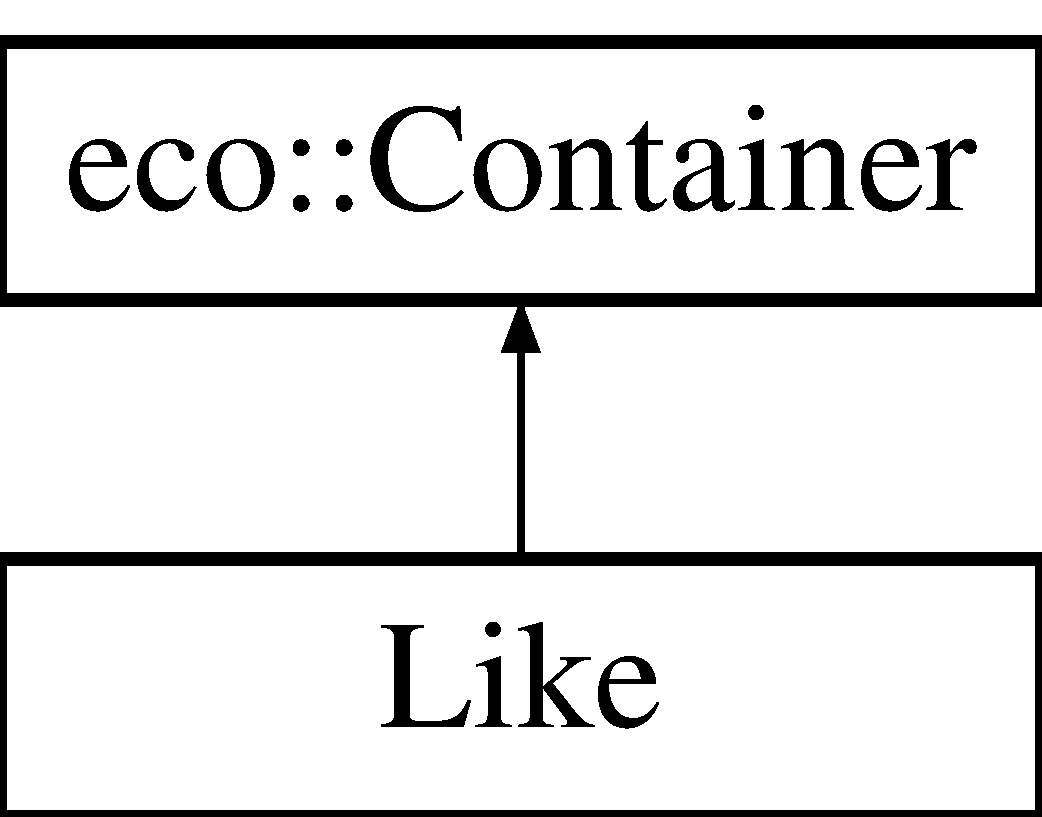
\includegraphics[height=2.000000cm]{structLike}
\end{center}
\end{figure}
\subsection*{Public Member Functions}
\begin{DoxyCompactItemize}
\item 
\hyperlink{structLike_ab1a696c6ed0f66421839b465d34a6da0}{Like} (unsigned int u\_\-spec\_\-id=0, int u\_\-like\_\-factor=0)
\begin{DoxyCompactList}\small\item\em default constructor \end{DoxyCompactList}\item 
bool \hyperlink{structLike_a507be8608c74775b568f093e15decbf1}{is\_\-full} ()
\begin{DoxyCompactList}\small\item\em is the like full \end{DoxyCompactList}\item 
\hypertarget{structLike_a0b36906c501104cbd13c0de9f02c2496}{
bool \hyperlink{structLike_a0b36906c501104cbd13c0de9f02c2496}{operator$<$} (const \hyperlink{structLike}{Like} \&lk)}
\label{structLike_a0b36906c501104cbd13c0de9f02c2496}

\begin{DoxyCompactList}\small\item\em \hyperlink{structLike}{Like} were sorted by ascendent spec\_\-id. \end{DoxyCompactList}\item 
\hypertarget{structLike_ae518b00028574d3ae76e9f8a77dfc846}{
bool \hyperlink{structLike_ae518b00028574d3ae76e9f8a77dfc846}{operator$>$} (const \hyperlink{structLike}{Like} \&lk)}
\label{structLike_ae518b00028574d3ae76e9f8a77dfc846}

\begin{DoxyCompactList}\small\item\em \hyperlink{structLike}{Like} were sorted by ascendent spec\_\-id. \end{DoxyCompactList}\item 
\hypertarget{structLike_aaf5f350734bfe2863099ee5a8310e313}{
bool \hyperlink{structLike_aaf5f350734bfe2863099ee5a8310e313}{operator==} (const \hyperlink{structLike}{Like} \&lk)}
\label{structLike_aaf5f350734bfe2863099ee5a8310e313}

\begin{DoxyCompactList}\small\item\em egual operator \end{DoxyCompactList}\item 
\hypertarget{structLike_a87ad505da19caa25877a86b172b2a036}{
bool \hyperlink{structLike_a87ad505da19caa25877a86b172b2a036}{operator!=} (const \hyperlink{structLike}{Like} \&lk)}
\label{structLike_a87ad505da19caa25877a86b172b2a036}

\begin{DoxyCompactList}\small\item\em not equal operator \end{DoxyCompactList}\end{DoxyCompactItemize}
\subsection*{Public Attributes}
\begin{DoxyCompactItemize}
\item 
\hypertarget{structLike_a5008dbeb4014c5f99618189cfd0ec57e}{
unsigned int \hyperlink{structLike_a5008dbeb4014c5f99618189cfd0ec57e}{liked\_\-spec\_\-id}}
\label{structLike_a5008dbeb4014c5f99618189cfd0ec57e}

\begin{DoxyCompactList}\small\item\em the species id liked \end{DoxyCompactList}\item 
int \hyperlink{structLike_aa10b4912394904201f7c75c4e9868a0f}{like\_\-factor}
\begin{DoxyCompactList}\small\item\em how much the species is liked \end{DoxyCompactList}\end{DoxyCompactItemize}
\subsection*{Friends}
\begin{DoxyCompactItemize}
\item 
\hypertarget{structLike_af6b658acce4e4592a0fcf1febecdccf8}{
std::ostream \& \hyperlink{structLike_af6b658acce4e4592a0fcf1febecdccf8}{operator$<$$<$} (std::ostream \&os, const \hyperlink{structLike}{Like} \&like)}
\label{structLike_af6b658acce4e4592a0fcf1febecdccf8}

\begin{DoxyCompactList}\small\item\em print liked\_\-species\_\-id and like\_\-factor \end{DoxyCompactList}\end{DoxyCompactItemize}


\subsection{Detailed Description}
how much a species is liked by another 

the liked\_\-spec\_\-id is the species id this species like and the like factor is how much he likes it. there is no way to know to which species belogns this like because they were inside the speciesinfo likings so it is enstablished that this like belongs to a precise species. in the example rabbit example: if this liking is referred to a rabbit the liked\_\-spec\_\-id is the id of a carrot and the like\_\-factor is how much from 1 to 100 the rabbit likes the carrot \begin{DoxySeeAlso}{See also}
\hyperlink{structSpeciesInfo}{SpeciesInfo} 

\hyperlink{structSpeciesInfo_a109b3e5acaf126bb8df9648b6c925542}{SpeciesInfo::likings} 
\end{DoxySeeAlso}


Definition at line 43 of file like.h.



\subsection{Constructor \& Destructor Documentation}
\hypertarget{structLike_ab1a696c6ed0f66421839b465d34a6da0}{
\index{Like@{Like}!Like@{Like}}
\index{Like@{Like}!Like@{Like}}
\subsubsection[{Like}]{\setlength{\rightskip}{0pt plus 5cm}Like::Like (
\begin{DoxyParamCaption}
\item[{unsigned int}]{u\_\-spec\_\-id = {\ttfamily 0}, }
\item[{int}]{u\_\-like\_\-factor = {\ttfamily 0}}
\end{DoxyParamCaption}
)}}
\label{structLike_ab1a696c6ed0f66421839b465d34a6da0}


default constructor 


\begin{DoxyParams}{Parameters}
{\em u\_\-spec\_\-id} & the species id \\
\hline
{\em u\_\-like\_\-factor} & the like factor \\
\hline
\end{DoxyParams}


Definition at line 25 of file like.cpp.



\subsection{Member Function Documentation}
\hypertarget{structLike_a507be8608c74775b568f093e15decbf1}{
\index{Like@{Like}!is\_\-full@{is\_\-full}}
\index{is\_\-full@{is\_\-full}!Like@{Like}}
\subsubsection[{is\_\-full}]{\setlength{\rightskip}{0pt plus 5cm}bool Like::is\_\-full (
\begin{DoxyParamCaption}
{}
\end{DoxyParamCaption}
)\hspace{0.3cm}{\ttfamily  \mbox{[}virtual\mbox{]}}}}
\label{structLike_a507be8608c74775b568f093e15decbf1}


is the like full 

controll if the liked\_\-spec\_\-id is $>$ 0 

Implements \hyperlink{classeco_1_1Container_aaba4667933eb47147b319f6daa7da5c2}{eco::Container}.



Definition at line 35 of file like.cpp.



\subsection{Member Data Documentation}
\hypertarget{structLike_aa10b4912394904201f7c75c4e9868a0f}{
\index{Like@{Like}!like\_\-factor@{like\_\-factor}}
\index{like\_\-factor@{like\_\-factor}!Like@{Like}}
\subsubsection[{like\_\-factor}]{\setlength{\rightskip}{0pt plus 5cm}int {\bf Like::like\_\-factor}}}
\label{structLike_aa10b4912394904201f7c75c4e9868a0f}


how much the species is liked 

positive is attraction

negative is repulsion

0 is 0 

Definition at line 85 of file like.h.



The documentation for this struct was generated from the following files:\begin{DoxyCompactItemize}
\item 
sources/like.h\item 
sources/like.cpp\end{DoxyCompactItemize}

\hypertarget{structLikeFactorCmp}{
\section{LikeFactorCmp Struct Reference}
\label{structLikeFactorCmp}\index{LikeFactorCmp@{LikeFactorCmp}}
}
\subsection*{Public Member Functions}
\begin{DoxyCompactItemize}
\item 
\hypertarget{structLikeFactorCmp_a53f50a486a3a15ab2c58032724ec26f7}{
bool {\bfseries operator()} (const \hyperlink{structLike}{Like} \&lhs, const \hyperlink{structLike}{Like} \&rhs)}
\label{structLikeFactorCmp_a53f50a486a3a15ab2c58032724ec26f7}

\end{DoxyCompactItemize}


\subsection{Detailed Description}


Definition at line 45 of file classcompares.hpp.



The documentation for this struct was generated from the following file:\begin{DoxyCompactItemize}
\item 
sources/\hyperlink{classcompares_8hpp}{classcompares.hpp}\end{DoxyCompactItemize}

\hypertarget{structLikeRefCmp}{
\section{LikeRefCmp Struct Reference}
\label{structLikeRefCmp}\index{LikeRefCmp@{LikeRefCmp}}
}


used in SpeciesInfo.h  




{\ttfamily \#include $<$classcompares.hpp$>$}

\subsection*{Public Member Functions}
\begin{DoxyCompactItemize}
\item 
\hypertarget{structLikeRefCmp_ac1b3915f2c65ec89adc4b0dba2fa4bb7}{
bool \hyperlink{structLikeRefCmp_ac1b3915f2c65ec89adc4b0dba2fa4bb7}{operator()} (const unsigned int \&lhs, const unsigned int \&rhs)}
\label{structLikeRefCmp_ac1b3915f2c65ec89adc4b0dba2fa4bb7}

\begin{DoxyCompactList}\small\item\em returns lhs$>$rhs \end{DoxyCompactList}\end{DoxyCompactItemize}


\subsection{Detailed Description}
used in SpeciesInfo.h 

compares the like\_\-factors of 2 like giving rhe biggerone. this is done to have the highest \hyperlink{structLike}{Like} first. \begin{DoxySeeAlso}{See also}
SpeciesInfo::m\_\-likings\_\-by\_\-lk\_\-factor 
\end{DoxySeeAlso}


Definition at line 36 of file classcompares.hpp.



The documentation for this struct was generated from the following file:\begin{DoxyCompactItemize}
\item 
sources/\hyperlink{classcompares_8hpp}{classcompares.hpp}\end{DoxyCompactItemize}

\hypertarget{structPopulationVariation}{
\section{PopulationVariation Struct Reference}
\label{structPopulationVariation}\index{PopulationVariation@{PopulationVariation}}
}


variation of population for a species in a subsystemcontainer  




{\ttfamily \#include $<$populationvariation.hpp$>$}

\subsection*{Public Types}
\begin{DoxyCompactItemize}
\item 
\hypertarget{structPopulationVariation_aae36f241d7c3048d87f581bce205fcd1}{
typedef std::pair$<$ unsigned int, unsigned int $>$ \hyperlink{structPopulationVariation_aae36f241d7c3048d87f581bce205fcd1}{coord\_\-tp}}
\label{structPopulationVariation_aae36f241d7c3048d87f581bce205fcd1}

\begin{DoxyCompactList}\small\item\em coordinates first x second y \end{DoxyCompactList}\end{DoxyCompactItemize}
\subsection*{Public Member Functions}
\begin{DoxyCompactItemize}
\item 
\hypertarget{structPopulationVariation_ae2c29030c2724faa35e1e423e9e4f6d3}{
\hyperlink{structPopulationVariation_ae2c29030c2724faa35e1e423e9e4f6d3}{PopulationVariation} (\hyperlink{structPopulationVariation_aae36f241d7c3048d87f581bce205fcd1}{coord\_\-tp} u\_\-coord\_\-tp, unsigned int u\_\-species\_\-id, int u\_\-variation, long int u\_\-abs\_\-time, float u\_\-rel\_\-time)}
\label{structPopulationVariation_ae2c29030c2724faa35e1e423e9e4f6d3}

\begin{DoxyCompactList}\small\item\em default contstructor \end{DoxyCompactList}\item 
\hypertarget{structPopulationVariation_a951e2ea39e8aa3024f514da0e79da185}{
\hyperlink{structPopulationVariation_a951e2ea39e8aa3024f514da0e79da185}{$\sim$PopulationVariation} ()}
\label{structPopulationVariation_a951e2ea39e8aa3024f514da0e79da185}

\begin{DoxyCompactList}\small\item\em deafult bestructor \end{DoxyCompactList}\end{DoxyCompactItemize}
\subsection*{Public Attributes}
\begin{DoxyCompactItemize}
\item 
\hypertarget{structPopulationVariation_a287eca2a34e5c68d3066456396408e03}{
\hyperlink{structPopulationVariation_aae36f241d7c3048d87f581bce205fcd1}{coord\_\-tp} \hyperlink{structPopulationVariation_a287eca2a34e5c68d3066456396408e03}{subs\_\-coord}}
\label{structPopulationVariation_a287eca2a34e5c68d3066456396408e03}

\begin{DoxyCompactList}\small\item\em subsystem coordinate in which occours the variation \end{DoxyCompactList}\item 
\hypertarget{structPopulationVariation_ad2f5ef6c52e0f3db00c5b5b66d7039e9}{
unsigned int \hyperlink{structPopulationVariation_ad2f5ef6c52e0f3db00c5b5b66d7039e9}{species\_\-id}}
\label{structPopulationVariation_ad2f5ef6c52e0f3db00c5b5b66d7039e9}

\begin{DoxyCompactList}\small\item\em the species of the animal that variate \end{DoxyCompactList}\item 
int \hyperlink{structPopulationVariation_a1dc7b506e2e3d3a0ba8ce0390a9d2c7d}{variation}
\begin{DoxyCompactList}\small\item\em the variation \end{DoxyCompactList}\item 
\hypertarget{structPopulationVariation_a49b63a98bc5c0d21ad541454afd9f39a}{
long int \hyperlink{structPopulationVariation_a49b63a98bc5c0d21ad541454afd9f39a}{abs\_\-time}}
\label{structPopulationVariation_a49b63a98bc5c0d21ad541454afd9f39a}

\begin{DoxyCompactList}\small\item\em absolute time of the variation \end{DoxyCompactList}\item 
\hypertarget{structPopulationVariation_a50a11ac13f338efd289b14b79ea87a02}{
float \hyperlink{structPopulationVariation_a50a11ac13f338efd289b14b79ea87a02}{rel\_\-time}}
\label{structPopulationVariation_a50a11ac13f338efd289b14b79ea87a02}

\begin{DoxyCompactList}\small\item\em relative time of the variation \end{DoxyCompactList}\end{DoxyCompactItemize}


\subsection{Detailed Description}
variation of population for a species in a subsystemcontainer 

this class contains the population variation for a species in a determinate subsystem container this class is layered inside \hyperlink{structStepLog}{StepLog} class and parsed by \hyperlink{classEcosystemContainer_a16d9614266ac07dc5252b1e731ab4712}{EcosystemContainer::step}; \begin{DoxySeeAlso}{See also}
\hyperlink{structStepLog}{StepLog} 

\hyperlink{classEcosystemContainer_a16d9614266ac07dc5252b1e731ab4712}{EcosystemContainer::step} 

\hyperlink{classSubsystemContainer}{SubsystemContainer} 

\hyperlink{structPopulationVariation_a287eca2a34e5c68d3066456396408e03}{subs\_\-coord} 

\hyperlink{structPopulationVariation_ad2f5ef6c52e0f3db00c5b5b66d7039e9}{species\_\-id} 

vartiation 
\end{DoxySeeAlso}


Definition at line 38 of file populationvariation.hpp.



\subsection{Member Data Documentation}
\hypertarget{structPopulationVariation_a1dc7b506e2e3d3a0ba8ce0390a9d2c7d}{
\index{PopulationVariation@{PopulationVariation}!variation@{variation}}
\index{variation@{variation}!PopulationVariation@{PopulationVariation}}
\subsubsection[{variation}]{\setlength{\rightskip}{0pt plus 5cm}int {\bf PopulationVariation::variation}}}
\label{structPopulationVariation_a1dc7b506e2e3d3a0ba8ce0390a9d2c7d}


the variation 

example: if the animal die variation is -\/1 

Definition at line 71 of file populationvariation.hpp.



The documentation for this struct was generated from the following file:\begin{DoxyCompactItemize}
\item 
sources/populationvariation.hpp\end{DoxyCompactItemize}

\hypertarget{structSubsystemContainer_1_1reproduction}{
\section{SubsystemContainer::reproduction Struct Reference}
\label{structSubsystemContainer_1_1reproduction}\index{SubsystemContainer::reproduction@{SubsystemContainer::reproduction}}
}


boost multyindex::ordered\_\-index tag  




{\ttfamily \#include $<$subsystemcontainer.h$>$}



\subsection{Detailed Description}
boost multyindex::ordered\_\-index tag 

Definition at line 85 of file subsystemcontainer.h.



The documentation for this struct was generated from the following file:\begin{DoxyCompactItemize}
\item 
sources/\hyperlink{subsystemcontainer_8h}{subsystemcontainer.h}\end{DoxyCompactItemize}

\hypertarget{structSubsystemContainer_1_1spec__id}{
\section{SubsystemContainer::spec\_\-id Struct Reference}
\label{structSubsystemContainer_1_1spec__id}\index{SubsystemContainer::spec\_\-id@{SubsystemContainer::spec\_\-id}}
}


boost multyindex::ordered\_\-index tag  




{\ttfamily \#include $<$subsystemcontainer.h$>$}



\subsection{Detailed Description}
boost multyindex::ordered\_\-index tag 

Definition at line 87 of file subsystemcontainer.h.



The documentation for this struct was generated from the following file:\begin{DoxyCompactItemize}
\item 
sources/\hyperlink{subsystemcontainer_8h}{subsystemcontainer.h}\end{DoxyCompactItemize}

\hypertarget{classSpecied}{
\section{Specied Class Reference}
\label{classSpecied}\index{Specied@{Specied}}
}


class \hyperlink{classSpecied}{Specied} the form of life as species belonger  




{\ttfamily \#include $<$specied.h$>$}

Inheritance diagram for Specied:\begin{figure}[H]
\begin{center}
\leavevmode
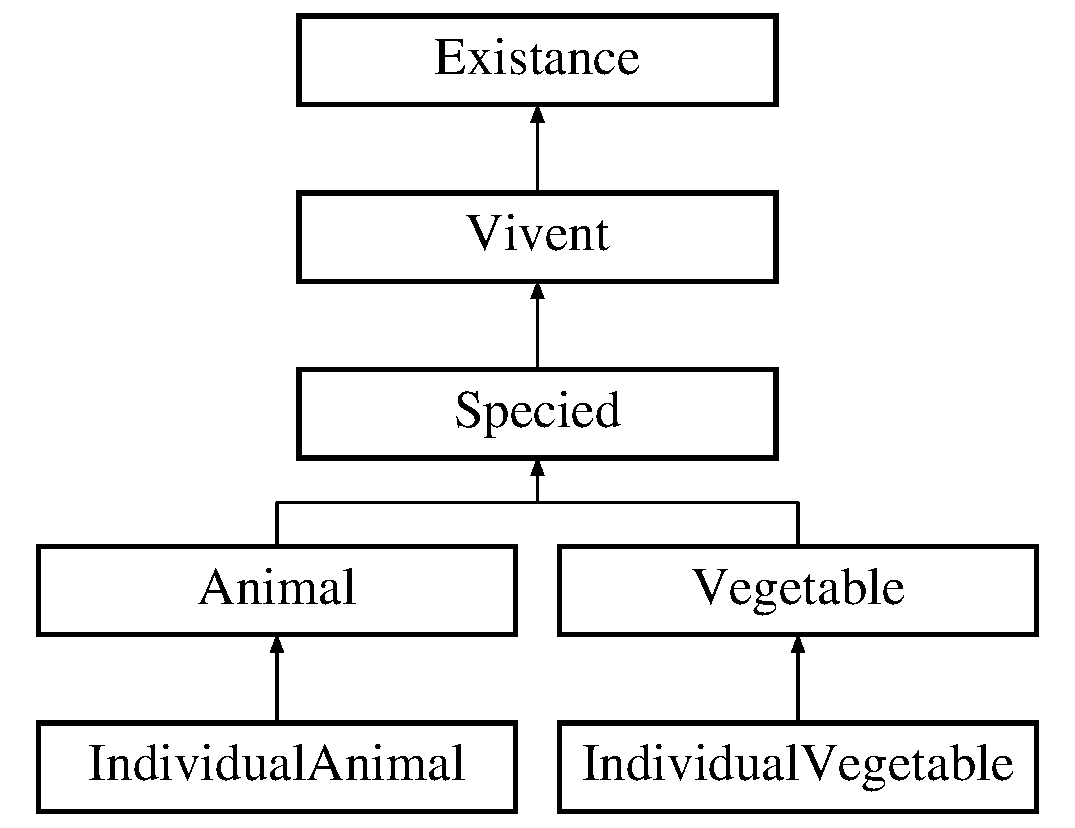
\includegraphics[height=5.000000cm]{classSpecied}
\end{center}
\end{figure}
\subsection*{Public Member Functions}
\begin{DoxyCompactItemize}
\item 
\hyperlink{classSpecied_aac5df03c9c0747691be7ff686d349da1}{Specied} (unsigned int u\_\-species\_\-id=0, std::string u\_\-species\_\-name=\char`\"{}no\_\-name\char`\"{}, unsigned int u\_\-life\_\-coast=1, unsigned int u\_\-health\_\-status=50, unsigned int u\_\-calories=1, float u\_\-life\_\-space=10)
\begin{DoxyCompactList}\small\item\em default constructor \end{DoxyCompactList}\item 
\hyperlink{classSpecied_aacc4458e62ccc9970178e8a40b703627}{$\sim$Specied} ()
\begin{DoxyCompactList}\small\item\em default destructor \end{DoxyCompactList}\item 
virtual bool \hyperlink{classSpecied_a2173ab978d5cd2c2de4e25a4d6eb3152}{is\_\-alive} ()
\begin{DoxyCompactList}\small\item\em is the \hyperlink{classSpecied}{Specied} form of life alive? \end{DoxyCompactList}\item 
unsigned int \& \hyperlink{classSpecied_a62459b7ffe5370668aeaa764786cc8cf}{species\_\-id} ()
\begin{DoxyCompactList}\small\item\em species id \end{DoxyCompactList}\item 
std::string \& \hyperlink{classSpecied_a104b980371c060ad8313ea0ef0a255d7}{species\_\-name} ()
\begin{DoxyCompactList}\small\item\em species name \end{DoxyCompactList}\item 
unsigned int \& \hyperlink{classSpecied_aa8cb3958e201a0689556c67df23ba38d}{life\_\-coast} ()
\begin{DoxyCompactList}\small\item\em life coast \end{DoxyCompactList}\item 
unsigned int \& \hyperlink{classSpecied_af53fa4047bf53367fe44c4a050863592}{health\_\-status} ()
\begin{DoxyCompactList}\small\item\em health statis \end{DoxyCompactList}\item 
unsigned int \& \hyperlink{classSpecied_a26cb3955f48f79b3d5f20a604ca3dd01}{calorie} ()
\begin{DoxyCompactList}\small\item\em calorie \end{DoxyCompactList}\item 
float \& \hyperlink{classSpecied_ab3f331fb396f5016d2297fcc2769375e}{life\_\-space} ()
\begin{DoxyCompactList}\small\item\em life space \end{DoxyCompactList}\item 
\hypertarget{classSpecied_a14bebd5e8b33ab0144f26e5887deaa56}{
unsigned int \hyperlink{classSpecied_a14bebd5e8b33ab0144f26e5887deaa56}{species\_\-id} () const }
\label{classSpecied_a14bebd5e8b33ab0144f26e5887deaa56}

\begin{DoxyCompactList}\small\item\em get the species\_\-id \end{DoxyCompactList}\item 
\hypertarget{classSpecied_a05225e19665a98ebb82e45887cc6632d}{
std::string \hyperlink{classSpecied_a05225e19665a98ebb82e45887cc6632d}{species\_\-name} () const }
\label{classSpecied_a05225e19665a98ebb82e45887cc6632d}

\begin{DoxyCompactList}\small\item\em get the species\_\-name \end{DoxyCompactList}\item 
\hypertarget{classSpecied_a7e442dcdc637e305d736de629d6dd63f}{
unsigned int \hyperlink{classSpecied_a7e442dcdc637e305d736de629d6dd63f}{life\_\-coast} () const }
\label{classSpecied_a7e442dcdc637e305d736de629d6dd63f}

\begin{DoxyCompactList}\small\item\em get the life\_\-coast \end{DoxyCompactList}\item 
\hypertarget{classSpecied_ad10fd46085a273d0402cabc97519a1d9}{
unsigned int \hyperlink{classSpecied_ad10fd46085a273d0402cabc97519a1d9}{health\_\-status} () const }
\label{classSpecied_ad10fd46085a273d0402cabc97519a1d9}

\begin{DoxyCompactList}\small\item\em get the health\_\-status \end{DoxyCompactList}\item 
\hypertarget{classSpecied_a7a0a72920da71c0177fcb4d36a700f70}{
unsigned int \hyperlink{classSpecied_a7a0a72920da71c0177fcb4d36a700f70}{calorie} () const }
\label{classSpecied_a7a0a72920da71c0177fcb4d36a700f70}

\begin{DoxyCompactList}\small\item\em get the calorie \end{DoxyCompactList}\item 
\hypertarget{classSpecied_aaf9d5d97e65ddb8e6ebe6d084eb47cf3}{
float \hyperlink{classSpecied_aaf9d5d97e65ddb8e6ebe6d084eb47cf3}{life\_\-space} () const }
\label{classSpecied_aaf9d5d97e65ddb8e6ebe6d084eb47cf3}

\begin{DoxyCompactList}\small\item\em get the life\_\-space \end{DoxyCompactList}\end{DoxyCompactItemize}
\subsection*{Private Attributes}
\begin{DoxyCompactItemize}
\item 
unsigned int \hyperlink{classSpecied_a7ddb2bbcdf287f07894da310b0a37dd0}{m\_\-species\_\-id}
\begin{DoxyCompactList}\small\item\em the numerical id of the species \end{DoxyCompactList}\item 
std::string \hyperlink{classSpecied_a028ecdb54e6a4f37406d3abcccf0de1c}{m\_\-species\_\-name}
\begin{DoxyCompactList}\small\item\em the name of the species \end{DoxyCompactList}\item 
unsigned int \hyperlink{classSpecied_acbfa5daa32bfb761a44f9d6e0763762e}{m\_\-life\_\-coast}
\begin{DoxyCompactList}\small\item\em the coast of life \end{DoxyCompactList}\item 
unsigned int \hyperlink{classSpecied_a7d716a70352c40bbe1ff3bd8c5719f29}{m\_\-health\_\-status}
\begin{DoxyCompactList}\small\item\em health status determine when an animal feels good \end{DoxyCompactList}\item 
unsigned int \hyperlink{classSpecied_ad02e0fffd55e2aa9227aa8034a05d374}{m\_\-calorie}
\begin{DoxyCompactList}\small\item\em calorie the nutritive power of the form of life \end{DoxyCompactList}\item 
float \hyperlink{classSpecied_a97ee13a155f2b2a58fed03279a2faa09}{m\_\-life\_\-space}
\begin{DoxyCompactList}\small\item\em occuped space in a quadro \end{DoxyCompactList}\end{DoxyCompactItemize}


\subsection{Detailed Description}
class \hyperlink{classSpecied}{Specied} the form of life as species belonger 

probabli the most important class of this library. it rappresents the form of life seen as belonging to a species so it contain all the characteristcs of animal of the same species like the : life coast and ... 

Definition at line 41 of file specied.h.



\subsection{Constructor \& Destructor Documentation}
\hypertarget{classSpecied_aac5df03c9c0747691be7ff686d349da1}{
\index{Specied@{Specied}!Specied@{Specied}}
\index{Specied@{Specied}!Specied@{Specied}}
\subsubsection[{Specied}]{\setlength{\rightskip}{0pt plus 5cm}Specied::Specied (
\begin{DoxyParamCaption}
\item[{unsigned int}]{u\_\-species\_\-id = {\ttfamily 0}, }
\item[{std::string}]{u\_\-species\_\-name = {\ttfamily \char`\"{}no\_\-name\char`\"{}}, }
\item[{unsigned int}]{u\_\-life\_\-coast = {\ttfamily 1}, }
\item[{unsigned int}]{u\_\-health\_\-status = {\ttfamily 50}, }
\item[{unsigned int}]{u\_\-calories = {\ttfamily 1}, }
\item[{float}]{u\_\-life\_\-space = {\ttfamily 10}}
\end{DoxyParamCaption}
)}}
\label{classSpecied_aac5df03c9c0747691be7ff686d349da1}


default constructor 

set private data members 

Definition at line 34 of file specied.cpp.

\hypertarget{classSpecied_aacc4458e62ccc9970178e8a40b703627}{
\index{Specied@{Specied}!$\sim$Specied@{$\sim$Specied}}
\index{$\sim$Specied@{$\sim$Specied}!Specied@{Specied}}
\subsubsection[{$\sim$Specied}]{\setlength{\rightskip}{0pt plus 5cm}Specied::$\sim$Specied (
\begin{DoxyParamCaption}
{}
\end{DoxyParamCaption}
)}}
\label{classSpecied_aacc4458e62ccc9970178e8a40b703627}


default destructor 

does nothing 

Definition at line 51 of file specied.cpp.



\subsection{Member Function Documentation}
\hypertarget{classSpecied_a26cb3955f48f79b3d5f20a604ca3dd01}{
\index{Specied@{Specied}!calorie@{calorie}}
\index{calorie@{calorie}!Specied@{Specied}}
\subsubsection[{calorie}]{\setlength{\rightskip}{0pt plus 5cm}unsigned int \& Specied::calorie (
\begin{DoxyParamCaption}
{}
\end{DoxyParamCaption}
)}}
\label{classSpecied_a26cb3955f48f79b3d5f20a604ca3dd01}


calorie 

\begin{DoxySeeAlso}{See also}
\hyperlink{classSpecied_ad02e0fffd55e2aa9227aa8034a05d374}{m\_\-calorie} 
\end{DoxySeeAlso}


Definition at line 85 of file specied.cpp.

\hypertarget{classSpecied_af53fa4047bf53367fe44c4a050863592}{
\index{Specied@{Specied}!health\_\-status@{health\_\-status}}
\index{health\_\-status@{health\_\-status}!Specied@{Specied}}
\subsubsection[{health\_\-status}]{\setlength{\rightskip}{0pt plus 5cm}unsigned int \& Specied::health\_\-status (
\begin{DoxyParamCaption}
{}
\end{DoxyParamCaption}
)}}
\label{classSpecied_af53fa4047bf53367fe44c4a050863592}


health statis 

\begin{DoxySeeAlso}{See also}
\hyperlink{classSpecied_a7d716a70352c40bbe1ff3bd8c5719f29}{m\_\-health\_\-status} 
\end{DoxySeeAlso}


Definition at line 80 of file specied.cpp.

\hypertarget{classSpecied_a2173ab978d5cd2c2de4e25a4d6eb3152}{
\index{Specied@{Specied}!is\_\-alive@{is\_\-alive}}
\index{is\_\-alive@{is\_\-alive}!Specied@{Specied}}
\subsubsection[{is\_\-alive}]{\setlength{\rightskip}{0pt plus 5cm}bool Specied::is\_\-alive (
\begin{DoxyParamCaption}
{}
\end{DoxyParamCaption}
)\hspace{0.3cm}{\ttfamily  \mbox{[}virtual\mbox{]}}}}
\label{classSpecied_a2173ab978d5cd2c2de4e25a4d6eb3152}


is the \hyperlink{classSpecied}{Specied} form of life alive? 

returns true if \hyperlink{classVivent_a5649888ad4779d5294fe7a6f57e4ecd4}{hp()} is $>$= 0; if the animal is not alive it will be removed. \begin{DoxySeeAlso}{See also}
\hyperlink{classEcosystemContainer_a16d9614266ac07dc5252b1e731ab4712}{EcosystemContainer::step()} 
\end{DoxySeeAlso}


Implements \hyperlink{classVivent_a253291090ae6207f8f51f8ff669d9d17}{Vivent}.



Reimplemented in \hyperlink{classIndividualAnimal_a78960ddab5b3649638ba6b97238edc06}{IndividualAnimal}.



Definition at line 60 of file specied.cpp.

\hypertarget{classSpecied_aa8cb3958e201a0689556c67df23ba38d}{
\index{Specied@{Specied}!life\_\-coast@{life\_\-coast}}
\index{life\_\-coast@{life\_\-coast}!Specied@{Specied}}
\subsubsection[{life\_\-coast}]{\setlength{\rightskip}{0pt plus 5cm}unsigned int \& Specied::life\_\-coast (
\begin{DoxyParamCaption}
{}
\end{DoxyParamCaption}
)}}
\label{classSpecied_aa8cb3958e201a0689556c67df23ba38d}


life coast 

\begin{DoxySeeAlso}{See also}
\hyperlink{classSpecied_acbfa5daa32bfb761a44f9d6e0763762e}{m\_\-life\_\-coast} 
\end{DoxySeeAlso}


Definition at line 75 of file specied.cpp.

\hypertarget{classSpecied_ab3f331fb396f5016d2297fcc2769375e}{
\index{Specied@{Specied}!life\_\-space@{life\_\-space}}
\index{life\_\-space@{life\_\-space}!Specied@{Specied}}
\subsubsection[{life\_\-space}]{\setlength{\rightskip}{0pt plus 5cm}float \& Specied::life\_\-space (
\begin{DoxyParamCaption}
{}
\end{DoxyParamCaption}
)}}
\label{classSpecied_ab3f331fb396f5016d2297fcc2769375e}


life space 

\begin{DoxySeeAlso}{See also}
\hyperlink{classSpecied_a97ee13a155f2b2a58fed03279a2faa09}{m\_\-life\_\-space} 
\end{DoxySeeAlso}


Definition at line 90 of file specied.cpp.

\hypertarget{classSpecied_a62459b7ffe5370668aeaa764786cc8cf}{
\index{Specied@{Specied}!species\_\-id@{species\_\-id}}
\index{species\_\-id@{species\_\-id}!Specied@{Specied}}
\subsubsection[{species\_\-id}]{\setlength{\rightskip}{0pt plus 5cm}unsigned int \& Specied::species\_\-id (
\begin{DoxyParamCaption}
{}
\end{DoxyParamCaption}
)}}
\label{classSpecied_a62459b7ffe5370668aeaa764786cc8cf}


species id 

\begin{DoxySeeAlso}{See also}
\hyperlink{classSpecied_a7ddb2bbcdf287f07894da310b0a37dd0}{m\_\-species\_\-id} 
\end{DoxySeeAlso}


Definition at line 65 of file specied.cpp.

\hypertarget{classSpecied_a104b980371c060ad8313ea0ef0a255d7}{
\index{Specied@{Specied}!species\_\-name@{species\_\-name}}
\index{species\_\-name@{species\_\-name}!Specied@{Specied}}
\subsubsection[{species\_\-name}]{\setlength{\rightskip}{0pt plus 5cm}std::string \& Specied::species\_\-name (
\begin{DoxyParamCaption}
{}
\end{DoxyParamCaption}
)}}
\label{classSpecied_a104b980371c060ad8313ea0ef0a255d7}


species name 

\begin{DoxySeeAlso}{See also}
\hyperlink{classSpecied_a028ecdb54e6a4f37406d3abcccf0de1c}{m\_\-species\_\-name} 
\end{DoxySeeAlso}


Definition at line 70 of file specied.cpp.



\subsection{Member Data Documentation}
\hypertarget{classSpecied_ad02e0fffd55e2aa9227aa8034a05d374}{
\index{Specied@{Specied}!m\_\-calorie@{m\_\-calorie}}
\index{m\_\-calorie@{m\_\-calorie}!Specied@{Specied}}
\subsubsection[{m\_\-calorie}]{\setlength{\rightskip}{0pt plus 5cm}unsigned int {\bf Specied::m\_\-calorie}\hspace{0.3cm}{\ttfamily  \mbox{[}private\mbox{]}}}}
\label{classSpecied_ad02e0fffd55e2aa9227aa8034a05d374}


calorie the nutritive power of the form of life 

each form of life, when eated, aliments the eater which can be only an animal (no carnivorous plants are modelled). the hp the eater receive are hp\_\-eaten $\ast$ calorie; 

Definition at line 161 of file specied.h.

\hypertarget{classSpecied_a7d716a70352c40bbe1ff3bd8c5719f29}{
\index{Specied@{Specied}!m\_\-health\_\-status@{m\_\-health\_\-status}}
\index{m\_\-health\_\-status@{m\_\-health\_\-status}!Specied@{Specied}}
\subsubsection[{m\_\-health\_\-status}]{\setlength{\rightskip}{0pt plus 5cm}unsigned int {\bf Specied::m\_\-health\_\-status}\hspace{0.3cm}{\ttfamily  \mbox{[}private\mbox{]}}}}
\label{classSpecied_a7d716a70352c40bbe1ff3bd8c5719f29}


health status determine when an animal feels good 

the health status has to be read as a percentage of the total hp reachable. over this percentage the form of life starts to feels good, so his libido rise in order to prefer the reproduction. no plant reproduction is included in this model! but for the future realises this data member in included in \hyperlink{classSpecied}{Specied} class 

Definition at line 154 of file specied.h.

\hypertarget{classSpecied_acbfa5daa32bfb761a44f9d6e0763762e}{
\index{Specied@{Specied}!m\_\-life\_\-coast@{m\_\-life\_\-coast}}
\index{m\_\-life\_\-coast@{m\_\-life\_\-coast}!Specied@{Specied}}
\subsubsection[{m\_\-life\_\-coast}]{\setlength{\rightskip}{0pt plus 5cm}unsigned int {\bf Specied::m\_\-life\_\-coast}\hspace{0.3cm}{\ttfamily  \mbox{[}private\mbox{]}}}}
\label{classSpecied_acbfa5daa32bfb761a44f9d6e0763762e}


the coast of life 

every time a specied is called it had to pay a life coast. this life coast is sottraed from the m\_\-hp when the life() member is called \begin{DoxySeeAlso}{See also}
live 
\end{DoxySeeAlso}


Definition at line 143 of file specied.h.

\hypertarget{classSpecied_a97ee13a155f2b2a58fed03279a2faa09}{
\index{Specied@{Specied}!m\_\-life\_\-space@{m\_\-life\_\-space}}
\index{m\_\-life\_\-space@{m\_\-life\_\-space}!Specied@{Specied}}
\subsubsection[{m\_\-life\_\-space}]{\setlength{\rightskip}{0pt plus 5cm}float {\bf Specied::m\_\-life\_\-space}\hspace{0.3cm}{\ttfamily  \mbox{[}private\mbox{]}}}}
\label{classSpecied_a97ee13a155f2b2a58fed03279a2faa09}


occuped space in a quadro 

the space occuped in a quadro in percentage. example: if m\_\-life\_\-space is 10 -\/$>$ no more than ten animal of this species can be hosted in a quadro 

Definition at line 168 of file specied.h.

\hypertarget{classSpecied_a7ddb2bbcdf287f07894da310b0a37dd0}{
\index{Specied@{Specied}!m\_\-species\_\-id@{m\_\-species\_\-id}}
\index{m\_\-species\_\-id@{m\_\-species\_\-id}!Specied@{Specied}}
\subsubsection[{m\_\-species\_\-id}]{\setlength{\rightskip}{0pt plus 5cm}unsigned int {\bf Specied::m\_\-species\_\-id}\hspace{0.3cm}{\ttfamily  \mbox{[}private\mbox{]}}}}
\label{classSpecied_a7ddb2bbcdf287f07894da310b0a37dd0}


the numerical id of the species 

this is the numerical id of the species and is used to identify the species in order to compute parameters and make statistics 

Definition at line 125 of file specied.h.

\hypertarget{classSpecied_a028ecdb54e6a4f37406d3abcccf0de1c}{
\index{Specied@{Specied}!m\_\-species\_\-name@{m\_\-species\_\-name}}
\index{m\_\-species\_\-name@{m\_\-species\_\-name}!Specied@{Specied}}
\subsubsection[{m\_\-species\_\-name}]{\setlength{\rightskip}{0pt plus 5cm}std::string {\bf Specied::m\_\-species\_\-name}\hspace{0.3cm}{\ttfamily  \mbox{[}private\mbox{]}}}}
\label{classSpecied_a028ecdb54e6a4f37406d3abcccf0de1c}


the name of the species 

the name of the species as it could be for a human. example: lion, bear, rabbit... this name is NOT used in any computational process, it's only for a better human understanding of the process

\begin{DoxySeeAlso}{See also}
\hyperlink{classSpecied_a7ddb2bbcdf287f07894da310b0a37dd0}{m\_\-species\_\-id} 
\end{DoxySeeAlso}


Definition at line 135 of file specied.h.



The documentation for this class was generated from the following files:\begin{DoxyCompactItemize}
\item 
sources/\hyperlink{specied_8h}{specied.h}\item 
sources/specied.cpp\end{DoxyCompactItemize}

\hypertarget{classSpeciesController}{
\section{SpeciesController Class Reference}
\label{classSpeciesController}\index{SpeciesController@{SpeciesController}}
}


contain info about the species in the ecosystem  




{\ttfamily \#include $<$speciescontroller.h$>$}

Inheritance diagram for SpeciesController:\begin{figure}[H]
\begin{center}
\leavevmode
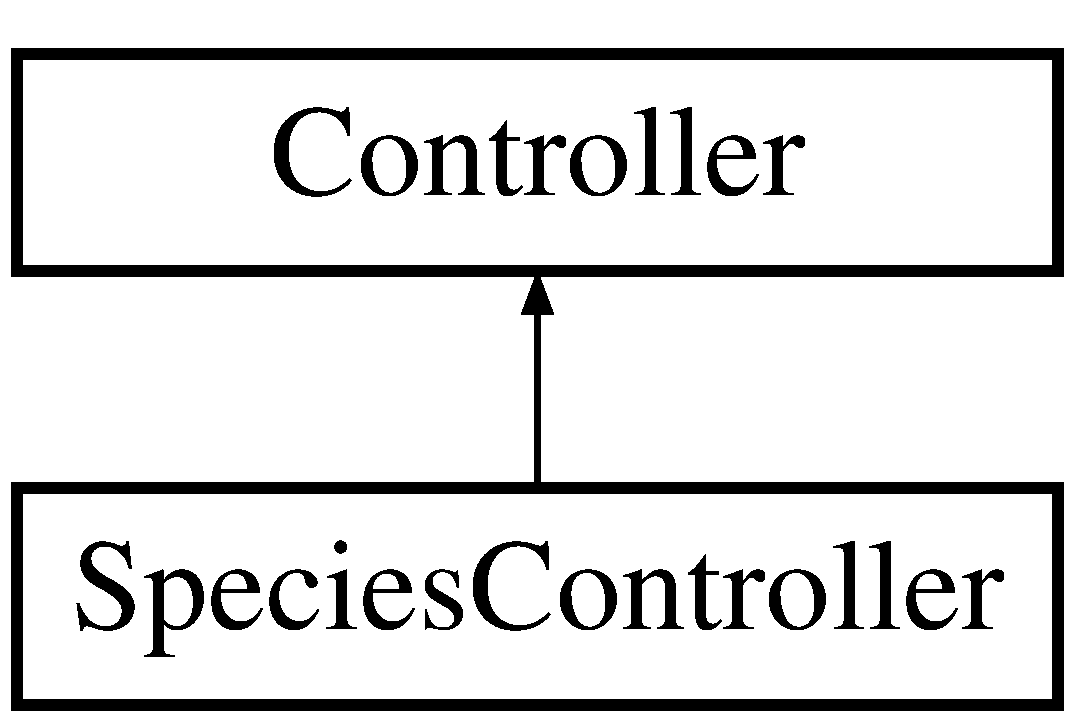
\includegraphics[height=2.000000cm]{classSpeciesController}
\end{center}
\end{figure}
\subsection*{Public Types}
\begin{DoxyCompactItemize}
\item 
typedef std::map$<$ unsigned int, \hyperlink{structSpeciesInfo}{SpeciesInfo} $>$ \hyperlink{classSpeciesController_a4b2e6ab3bbcf3d53a4588967eb615ff7}{infos\_\-tp}
\begin{DoxyCompactList}\small\item\em the type of the infos map \end{DoxyCompactList}\item 
typedef std::map$<$ unsigned int, \hyperlink{structSpeciesInfo}{SpeciesInfo} $>$::iterator \hyperlink{classSpeciesController_a4026e8acb68f2b04ecc13bb20c68008a}{infos\_\-it}
\begin{DoxyCompactList}\small\item\em info iterator \end{DoxyCompactList}\item 
typedef std::map$<$ unsigned int, \hyperlink{structSpeciesInfo}{SpeciesInfo} $>$::const\_\-iterator \hyperlink{classSpeciesController_a0dc92662511aca888d67516eb87b6260}{infos\_\-const\_\-it}
\begin{DoxyCompactList}\small\item\em info const\_\-iterator \end{DoxyCompactList}\end{DoxyCompactItemize}
\subsection*{Public Member Functions}
\begin{DoxyCompactItemize}
\item 
\hyperlink{classSpeciesController_a5af2abb109a098e7f6b2d16823d16458}{SpeciesController} (unsigned int u\_\-species\_\-number=0)
\begin{DoxyCompactList}\small\item\em default contructor \end{DoxyCompactList}\item 
\hypertarget{classSpeciesController_a0a6d3bdb642f21c63a619087ac38e073}{
\hyperlink{classSpeciesController_a0a6d3bdb642f21c63a619087ac38e073}{$\sim$SpeciesController} ()}
\label{classSpeciesController_a0a6d3bdb642f21c63a619087ac38e073}

\begin{DoxyCompactList}\small\item\em default destrictor \end{DoxyCompactList}\item 
virtual bool \hyperlink{classSpeciesController_a82ca8bb4c8f99e8b1151990ef293e39a}{check} ()
\begin{DoxyCompactList}\small\item\em check if the controll is completed \end{DoxyCompactList}\item 
\hypertarget{classSpeciesController_ae12020f4f91bc487e447fe6225bc138d}{
std::pair$<$ \hyperlink{classSpeciesController_a4026e8acb68f2b04ecc13bb20c68008a}{infos\_\-it}, bool $>$ \hyperlink{classSpeciesController_ae12020f4f91bc487e447fe6225bc138d}{insert} (const \hyperlink{structSpeciesInfo}{SpeciesInfo} \&spi)}
\label{classSpeciesController_ae12020f4f91bc487e447fe6225bc138d}

\begin{DoxyCompactList}\small\item\em insert a species info \end{DoxyCompactList}\item 
\hyperlink{classSpeciesController_a0dc92662511aca888d67516eb87b6260}{infos\_\-const\_\-it} \hyperlink{classSpeciesController_a1d9d5598574e4dc9c7023440a7a0245b}{get\_\-info} (const unsigned int u\_\-spec\_\-id)
\begin{DoxyCompactList}\small\item\em get infos about a species \end{DoxyCompactList}\item 
\hypertarget{classSpeciesController_aabe704fcc426ad3ec1ae46d0ed7e667d}{
const \hyperlink{structSpeciesInfo}{SpeciesInfo} \& \hyperlink{classSpeciesController_aabe704fcc426ad3ec1ae46d0ed7e667d}{get\_\-info\_\-ref} (const unsigned int u\_\-spec\_\-id) const }
\label{classSpeciesController_aabe704fcc426ad3ec1ae46d0ed7e667d}

\begin{DoxyCompactList}\small\item\em get the reference to the species info whith u\_\-spec\_\-id as species\_\-id \end{DoxyCompactList}\item 
int \hyperlink{classSpeciesController_a467ef1497b83bb2ae5f0990cab611c34}{get\_\-like\_\-factor} (const unsigned int predator\_\-spec\_\-id, const unsigned int prey\_\-spec\_\-id)
\begin{DoxyCompactList}\small\item\em get like\_\-factor \end{DoxyCompactList}\item 
const std::map$<$ unsigned int, \hyperlink{structSpeciesInfo}{SpeciesInfo} $>$ \& \hyperlink{classSpeciesController_ae3173c4b361dcbe2e8efb0c0f6e80486}{get\_\-infos} () const 
\begin{DoxyCompactList}\small\item\em get the species infos \end{DoxyCompactList}\item 
\hypertarget{classSpeciesController_af22a0989362a058602cc7e039ce0182f}{
std::map$<$ unsigned int, \hyperlink{structSpeciesInfo}{SpeciesInfo} $>$ \& \hyperlink{classSpeciesController_af22a0989362a058602cc7e039ce0182f}{get\_\-infos} ()}
\label{classSpeciesController_af22a0989362a058602cc7e039ce0182f}

\begin{DoxyCompactList}\small\item\em get the infos \end{DoxyCompactList}\item 
\hypertarget{classSpeciesController_abd757b3bd462b28307a93e3fe1857832}{
unsigned int \hyperlink{classSpeciesController_abd757b3bd462b28307a93e3fe1857832}{species\_\-number} ()}
\label{classSpeciesController_abd757b3bd462b28307a93e3fe1857832}

\begin{DoxyCompactList}\small\item\em get the total species number \end{DoxyCompactList}\end{DoxyCompactItemize}
\subsection*{Private Member Functions}
\begin{DoxyCompactItemize}
\item 
bool \hyperlink{classSpeciesController_a67380eb665706237de2207d46125a82b}{string\_\-parser} (const std::string \&str, \hyperlink{structSpeciesInfo}{SpeciesInfo} \&spi)
\begin{DoxyCompactList}\small\item\em string parser \end{DoxyCompactList}\end{DoxyCompactItemize}
\subsection*{Private Attributes}
\begin{DoxyCompactItemize}
\item 
\hypertarget{classSpeciesController_aeff7a0500fcf53ad83f4d175adaef85d}{
unsigned int \hyperlink{classSpeciesController_aeff7a0500fcf53ad83f4d175adaef85d}{m\_\-species\_\-number}}
\label{classSpeciesController_aeff7a0500fcf53ad83f4d175adaef85d}

\begin{DoxyCompactList}\small\item\em total number of species in the ecosystem \end{DoxyCompactList}\item 
std::map$<$ unsigned int, \hyperlink{structSpeciesInfo}{SpeciesInfo} $>$ \hyperlink{classSpeciesController_a4e439ccd41d6143680b7a89bd985c8ad}{m\_\-infos}
\begin{DoxyCompactList}\small\item\em container of species info \end{DoxyCompactList}\end{DoxyCompactItemize}
\subsection*{Friends}
\begin{DoxyCompactItemize}
\item 
std::ifstream \& \hyperlink{classSpeciesController_aeb4b1409fd5367b5925f1552ee935aa8}{operator$>$$>$} (std::ifstream \&is, \hyperlink{classSpeciesController}{SpeciesController} \&sa)
\begin{DoxyCompactList}\small\item\em operator $>$$>$ \end{DoxyCompactList}\item 
std::istream \& \hyperlink{classSpeciesController_a26bec2c9a56999b0e717d0b225fbc942}{operator$>$$>$} (std::istream \&is, \hyperlink{classSpeciesController}{SpeciesController} \&sa)
\begin{DoxyCompactList}\small\item\em operator $>$$>$ \end{DoxyCompactList}\item 
\hypertarget{classSpeciesController_abb0fb135115ac68cbc84f562a861d81b}{
std::ostream \& \hyperlink{classSpeciesController_abb0fb135115ac68cbc84f562a861d81b}{operator$<$$<$} (std::ostream \&is, const \hyperlink{classSpeciesController}{SpeciesController} \&sa)}
\label{classSpeciesController_abb0fb135115ac68cbc84f562a861d81b}

\begin{DoxyCompactList}\small\item\em operator $<$$<$ \end{DoxyCompactList}\end{DoxyCompactItemize}


\subsection{Detailed Description}
contain info about the species in the ecosystem 

this class contains all the information about the species present in the ecosystem. this class is the UNIQUE reference for the features of a species. this is class inside the ecosystem to provide the values relative the species. in this way al the form of life in the ecosystem of the same species have the same value for dm relative to the species.

this class is also used to determine how much species like each others. for like we intend \char`\"{}to prefer for dinner\char`\"{}.

particular attention was given to the affidability and to the rightness of the data field inserted. controll statement preservers from multiple insertions of lines and wrong likes. the computational coast is hight but this element has to be build rightly and only one time for ecosystem so is a good fee to pay. 

Definition at line 61 of file speciescontroller.h.



\subsection{Member Typedef Documentation}
\hypertarget{classSpeciesController_a0dc92662511aca888d67516eb87b6260}{
\index{SpeciesController@{SpeciesController}!infos\_\-const\_\-it@{infos\_\-const\_\-it}}
\index{infos\_\-const\_\-it@{infos\_\-const\_\-it}!SpeciesController@{SpeciesController}}
\subsubsection[{infos\_\-const\_\-it}]{\setlength{\rightskip}{0pt plus 5cm}typedef std::map$<$unsigned int, {\bf SpeciesInfo}$>$::const\_\-iterator {\bf SpeciesController::infos\_\-const\_\-it}}}
\label{classSpeciesController_a0dc92662511aca888d67516eb87b6260}


info const\_\-iterator 

\begin{DoxySeeAlso}{See also}
\hyperlink{classSpeciesController_a4e439ccd41d6143680b7a89bd985c8ad}{m\_\-infos} 
\end{DoxySeeAlso}


Definition at line 81 of file speciescontroller.h.

\hypertarget{classSpeciesController_a4026e8acb68f2b04ecc13bb20c68008a}{
\index{SpeciesController@{SpeciesController}!infos\_\-it@{infos\_\-it}}
\index{infos\_\-it@{infos\_\-it}!SpeciesController@{SpeciesController}}
\subsubsection[{infos\_\-it}]{\setlength{\rightskip}{0pt plus 5cm}typedef std::map$<$unsigned int, {\bf SpeciesInfo}$>$::iterator {\bf SpeciesController::infos\_\-it}}}
\label{classSpeciesController_a4026e8acb68f2b04ecc13bb20c68008a}


info iterator 

\begin{DoxySeeAlso}{See also}
\hyperlink{classSpeciesController_a4e439ccd41d6143680b7a89bd985c8ad}{m\_\-infos} 
\end{DoxySeeAlso}


Definition at line 75 of file speciescontroller.h.

\hypertarget{classSpeciesController_a4b2e6ab3bbcf3d53a4588967eb615ff7}{
\index{SpeciesController@{SpeciesController}!infos\_\-tp@{infos\_\-tp}}
\index{infos\_\-tp@{infos\_\-tp}!SpeciesController@{SpeciesController}}
\subsubsection[{infos\_\-tp}]{\setlength{\rightskip}{0pt plus 5cm}typedef std::map$<$unsigned int, {\bf SpeciesInfo}$>$ {\bf SpeciesController::infos\_\-tp}}}
\label{classSpeciesController_a4b2e6ab3bbcf3d53a4588967eb615ff7}


the type of the infos map 

typedef std::map$<$unsigned int, SpeciesInfo$>$ 

Definition at line 69 of file speciescontroller.h.



\subsection{Constructor \& Destructor Documentation}
\hypertarget{classSpeciesController_a5af2abb109a098e7f6b2d16823d16458}{
\index{SpeciesController@{SpeciesController}!SpeciesController@{SpeciesController}}
\index{SpeciesController@{SpeciesController}!SpeciesController@{SpeciesController}}
\subsubsection[{SpeciesController}]{\setlength{\rightskip}{0pt plus 5cm}SpecCon::SpeciesController (
\begin{DoxyParamCaption}
\item[{unsigned int}]{u\_\-species\_\-number = {\ttfamily 0}}
\end{DoxyParamCaption}
)}}
\label{classSpeciesController_a5af2abb109a098e7f6b2d16823d16458}


default contructor 

if no u\_\-species\_\-number is passed will set to 0 and \hyperlink{classSpeciesController_a82ca8bb4c8f99e8b1151990ef293e39a}{check()} will fail 

Definition at line 40 of file speciescontroller.cpp.



\subsection{Member Function Documentation}
\hypertarget{classSpeciesController_a82ca8bb4c8f99e8b1151990ef293e39a}{
\index{SpeciesController@{SpeciesController}!check@{check}}
\index{check@{check}!SpeciesController@{SpeciesController}}
\subsubsection[{check}]{\setlength{\rightskip}{0pt plus 5cm}bool SpecCon::check (
\begin{DoxyParamCaption}
{}
\end{DoxyParamCaption}
)\hspace{0.3cm}{\ttfamily  \mbox{[}virtual\mbox{]}}}}
\label{classSpeciesController_a82ca8bb4c8f99e8b1151990ef293e39a}


check if the controll is completed 

\begin{DoxyReturn}{Returns}
true only if those condition are simultaneus:
\begin{DoxyItemize}
\item total species number is not 0
\item the number of SpeciesInfos coincide with the number of species in ecosystem
\item every \hyperlink{structSpeciesInfo}{SpeciesInfo} returns true if is\_\-full() is called 
\end{DoxyItemize}
\end{DoxyReturn}
\begin{DoxySeeAlso}{See also}
\hyperlink{structSpeciesInfo_a3d012834e84c8d878436a739f141f154}{SpeciesInfo::is\_\-full()} 
\end{DoxySeeAlso}


Implements \hyperlink{classController_abcf0d0905edc35ee09dc761bd2878d6a}{Controller}.



Definition at line 49 of file speciescontroller.cpp.

\hypertarget{classSpeciesController_a1d9d5598574e4dc9c7023440a7a0245b}{
\index{SpeciesController@{SpeciesController}!get\_\-info@{get\_\-info}}
\index{get\_\-info@{get\_\-info}!SpeciesController@{SpeciesController}}
\subsubsection[{get\_\-info}]{\setlength{\rightskip}{0pt plus 5cm}{\bf SpecCon::infos\_\-const\_\-it} SpecCon::get\_\-info (
\begin{DoxyParamCaption}
\item[{const unsigned int}]{u\_\-spec\_\-id}
\end{DoxyParamCaption}
)}}
\label{classSpeciesController_a1d9d5598574e4dc9c7023440a7a0245b}


get infos about a species 

\begin{DoxyReturn}{Returns}
a const iterator to a pair which the second member is the \hyperlink{structSpeciesInfo}{SpeciesInfo}. if the species does not exists returns an iterator to m\_\-infos.end(); 
\end{DoxyReturn}


Definition at line 178 of file speciescontroller.cpp.

\hypertarget{classSpeciesController_ae3173c4b361dcbe2e8efb0c0f6e80486}{
\index{SpeciesController@{SpeciesController}!get\_\-infos@{get\_\-infos}}
\index{get\_\-infos@{get\_\-infos}!SpeciesController@{SpeciesController}}
\subsubsection[{get\_\-infos}]{\setlength{\rightskip}{0pt plus 5cm}const std::map$<$ unsigned int, {\bf SpeciesInfo} $>$ \& SpecCon::get\_\-infos (
\begin{DoxyParamCaption}
{}
\end{DoxyParamCaption}
) const}}
\label{classSpeciesController_ae3173c4b361dcbe2e8efb0c0f6e80486}


get the species infos 

\begin{DoxyReturn}{Returns}
a const reference to species infos container, which is a map; 
\end{DoxyReturn}


Definition at line 225 of file speciescontroller.cpp.

\hypertarget{classSpeciesController_a467ef1497b83bb2ae5f0990cab611c34}{
\index{SpeciesController@{SpeciesController}!get\_\-like\_\-factor@{get\_\-like\_\-factor}}
\index{get\_\-like\_\-factor@{get\_\-like\_\-factor}!SpeciesController@{SpeciesController}}
\subsubsection[{get\_\-like\_\-factor}]{\setlength{\rightskip}{0pt plus 5cm}int SpecCon::get\_\-like\_\-factor (
\begin{DoxyParamCaption}
\item[{const unsigned int}]{predator\_\-spec\_\-id, }
\item[{const unsigned int}]{prey\_\-spec\_\-id}
\end{DoxyParamCaption}
)}}
\label{classSpeciesController_a467ef1497b83bb2ae5f0990cab611c34}


get like\_\-factor 


\begin{DoxyParams}{Parameters}
{\em predator\_\-spec\_\-id} & the species id of the Species which wants to eat. \\
\hline
{\em prey\_\-spec\_\-id} & the species id that will be eaten \\
\hline
\end{DoxyParams}
\begin{DoxyReturn}{Returns}
the like factor. how much the predator like the prey
\end{DoxyReturn}
\begin{DoxySeeAlso}{See also}
\hyperlink{structLike_aa10b4912394904201f7c75c4e9868a0f}{Like::like\_\-factor} 
\end{DoxySeeAlso}


Definition at line 202 of file speciescontroller.cpp.

\hypertarget{classSpeciesController_a67380eb665706237de2207d46125a82b}{
\index{SpeciesController@{SpeciesController}!string\_\-parser@{string\_\-parser}}
\index{string\_\-parser@{string\_\-parser}!SpeciesController@{SpeciesController}}
\subsubsection[{string\_\-parser}]{\setlength{\rightskip}{0pt plus 5cm}bool SpecCon::string\_\-parser (
\begin{DoxyParamCaption}
\item[{const std::string \&}]{str, }
\item[{{\bf SpeciesInfo} \&}]{spi}
\end{DoxyParamCaption}
)\hspace{0.3cm}{\ttfamily  \mbox{[}private\mbox{]}}}}
\label{classSpeciesController_a67380eb665706237de2207d46125a82b}


string parser 

parse an input line and put's the input in the spi field

Input Format: the line passed contains numerous info divided by a \char`\"{}$|$\char`\"{} here's the order of the fields: (note that we are in C++ so the first element has position 0)


\begin{DoxyItemize}
\item species\_\-id (0 is not valid)
\item species\_\-name
\item \char`\"{}vegetable\char`\"{} or \char`\"{}animal\char`\"{}
\item life\_\-coast
\item health\_\-status
\item calories
\item life\_\-space
\end{DoxyItemize}

after 6 tokens have to insert the \hyperlink{structLike}{Like} of the species in the format: liked\_\-species-\/like\_\-factor. pay attention to the \char`\"{}-\/\char`\"{}. as usual every \hyperlink{structLike}{Like} has to be separated by \char`\"{}$|$\char`\"{}. return m\_\-infos; if the numbers of Likes is not = to the total species number in the ecosystem -\/ 1 . the function will return false;

example: if we have 3 species in the ecosystem (1 is lion, 2 is gazzella , 3 is grass):

\char`\"{}1$|$lion$|$animal$|$10$|$50$|$1$|$45$|$2-\/50$|$3-\/0\char`\"{}


\begin{DoxyParams}{Parameters}
{\em str} & string containing the data \\
\hline
{\em spi} & \hyperlink{structSpeciesInfo}{SpeciesInfo} in which put data \\
\hline
\end{DoxyParams}
\begin{DoxyReturn}{Returns}
true if the string were well done, false if the string wasn't formatted correctly 
\end{DoxyReturn}
\begin{DoxySeeAlso}{See also}
operator$>$$>$ 
\end{DoxySeeAlso}


Definition at line 235 of file speciescontroller.cpp.



\subsection{Friends And Related Function Documentation}
\hypertarget{classSpeciesController_aeb4b1409fd5367b5925f1552ee935aa8}{
\index{SpeciesController@{SpeciesController}!operator$>$$>$@{operator$>$$>$}}
\index{operator$>$$>$@{operator$>$$>$}!SpeciesController@{SpeciesController}}
\subsubsection[{operator$>$$>$}]{\setlength{\rightskip}{0pt plus 5cm}std::ifstream\& operator$>$$>$ (
\begin{DoxyParamCaption}
\item[{std::ifstream \&}]{is, }
\item[{{\bf SpeciesController} \&}]{sa}
\end{DoxyParamCaption}
)\hspace{0.3cm}{\ttfamily  \mbox{[}friend\mbox{]}}}}
\label{classSpeciesController_aeb4b1409fd5367b5925f1552ee935aa8}


operator $>$$>$ 

load all \hyperlink{structSpeciesInfo}{SpeciesInfo} for all species. take the first line of the stream and passes it a string\_\-parser. to be used whith filestream \begin{DoxySeeAlso}{See also}
\hyperlink{classSpeciesController_a67380eb665706237de2207d46125a82b}{string\_\-parser} for the data format; 
\end{DoxySeeAlso}


Definition at line 571 of file speciescontroller.cpp.

\hypertarget{classSpeciesController_a26bec2c9a56999b0e717d0b225fbc942}{
\index{SpeciesController@{SpeciesController}!operator$>$$>$@{operator$>$$>$}}
\index{operator$>$$>$@{operator$>$$>$}!SpeciesController@{SpeciesController}}
\subsubsection[{operator$>$$>$}]{\setlength{\rightskip}{0pt plus 5cm}std::istream\& operator$>$$>$ (
\begin{DoxyParamCaption}
\item[{std::istream \&}]{is, }
\item[{{\bf SpeciesController} \&}]{sa}
\end{DoxyParamCaption}
)\hspace{0.3cm}{\ttfamily  \mbox{[}friend\mbox{]}}}}
\label{classSpeciesController_a26bec2c9a56999b0e717d0b225fbc942}


operator $>$$>$ 

load all \hyperlink{structSpeciesInfo}{SpeciesInfo} for all species. to be used whith std::cin, ask for the fields an compose a line to pass to line\_\-parser then if the line is well composed insert the \hyperlink{structSpeciesInfo}{SpeciesInfo} 

Definition at line 654 of file speciescontroller.cpp.



\subsection{Member Data Documentation}
\hypertarget{classSpeciesController_a4e439ccd41d6143680b7a89bd985c8ad}{
\index{SpeciesController@{SpeciesController}!m\_\-infos@{m\_\-infos}}
\index{m\_\-infos@{m\_\-infos}!SpeciesController@{SpeciesController}}
\subsubsection[{m\_\-infos}]{\setlength{\rightskip}{0pt plus 5cm}std::map$<$unsigned int, {\bf SpeciesInfo}$>$ {\bf SpeciesController::m\_\-infos}\hspace{0.3cm}{\ttfamily  \mbox{[}private\mbox{]}}}}
\label{classSpeciesController_a4e439ccd41d6143680b7a89bd985c8ad}


container of species info 

species infos were sorted by spec\_\-id \begin{DoxySeeAlso}{See also}
\hyperlink{structSpeciesInfo}{SpeciesInfo} 

\hyperlink{structSpeciesInfo_ab9716bf0081511ea866d49e173bd0554}{SpeciesInfo::operator$<$} 
\end{DoxySeeAlso}


Definition at line 214 of file speciescontroller.h.



The documentation for this class was generated from the following files:\begin{DoxyCompactItemize}
\item 
sources/\hyperlink{speciescontroller_8h}{speciescontroller.h}\item 
sources/speciescontroller.cpp\end{DoxyCompactItemize}

\hypertarget{structSpeciesInfo}{
\section{SpeciesInfo Struct Reference}
\label{structSpeciesInfo}\index{SpeciesInfo@{SpeciesInfo}}
}


species info containers  




{\ttfamily \#include $<$speciesinfo.h$>$}

Inheritance diagram for SpeciesInfo:\begin{figure}[H]
\begin{center}
\leavevmode
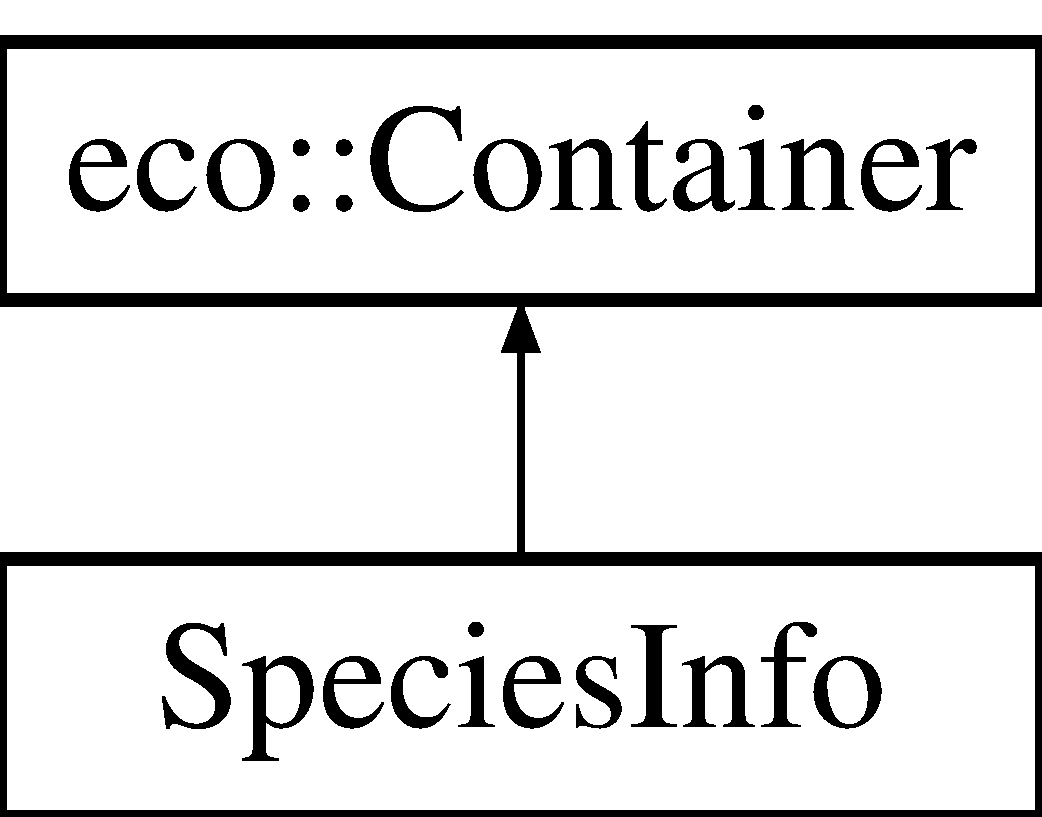
\includegraphics[height=2.000000cm]{structSpeciesInfo}
\end{center}
\end{figure}
\subsection*{Public Types}
\begin{DoxyCompactItemize}
\item 
\hypertarget{structSpeciesInfo_aa70735bd441c2465b36bef55cfabb1bf}{
typedef std::map$<$ unsigned int, \hyperlink{structLike}{Like} $>$ \hyperlink{structSpeciesInfo_aa70735bd441c2465b36bef55cfabb1bf}{likings\_\-map\_\-tp}}
\label{structSpeciesInfo_aa70735bd441c2465b36bef55cfabb1bf}

\begin{DoxyCompactList}\small\item\em likings type \end{DoxyCompactList}\item 
\hypertarget{structSpeciesInfo_a06dc895ad5da1d736e971e0690194c5f}{
typedef likings\_\-map\_\-tp::iterator \hyperlink{structSpeciesInfo_a06dc895ad5da1d736e971e0690194c5f}{likings\_\-it}}
\label{structSpeciesInfo_a06dc895ad5da1d736e971e0690194c5f}

\begin{DoxyCompactList}\small\item\em iteratore per membro di likings \end{DoxyCompactList}\item 
\hypertarget{structSpeciesInfo_acd0e4c451993ca95135fcdc8840c344b}{
typedef likings\_\-map\_\-tp::const\_\-iterator \hyperlink{structSpeciesInfo_acd0e4c451993ca95135fcdc8840c344b}{likings\_\-const\_\-it}}
\label{structSpeciesInfo_acd0e4c451993ca95135fcdc8840c344b}

\begin{DoxyCompactList}\small\item\em iteratore constante per membro di likings \end{DoxyCompactList}\item 
typedef std::multiset$<$ \hyperlink{structLike}{Like}, \hyperlink{structLikeFactorCmp}{LikeFactorCmp} $>$ \hyperlink{structSpeciesInfo_aab6fabec09f9eb5a26e680d1d6f9d037}{likings\_\-by\_\-lk\_\-factor\_\-tp}
\begin{DoxyCompactList}\small\item\em multimap sorted by like\_\-factor \end{DoxyCompactList}\item 
\hypertarget{structSpeciesInfo_ac9d1365506aed6cd1daf2ba982a80473}{
typedef likings\_\-by\_\-lk\_\-factor\_\-tp::iterator \hyperlink{structSpeciesInfo_ac9d1365506aed6cd1daf2ba982a80473}{likings\_\-by\_\-lk\_\-factor\_\-iterator}}
\label{structSpeciesInfo_ac9d1365506aed6cd1daf2ba982a80473}

\begin{DoxyCompactList}\small\item\em iterator to access like sorted by lk factor \end{DoxyCompactList}\item 
\hypertarget{structSpeciesInfo_a1e10640a53fd3c1524fcafcdfe3d1a10}{
typedef likings\_\-by\_\-lk\_\-factor\_\-tp::const\_\-iterator \hyperlink{structSpeciesInfo_a1e10640a53fd3c1524fcafcdfe3d1a10}{likings\_\-by\_\-lk\_\-factor\_\-const\_\-iterator}}
\label{structSpeciesInfo_a1e10640a53fd3c1524fcafcdfe3d1a10}

\begin{DoxyCompactList}\small\item\em const iterator to access like sorted by lk factor \end{DoxyCompactList}\end{DoxyCompactItemize}
\subsection*{Public Member Functions}
\begin{DoxyCompactItemize}
\item 
\hypertarget{structSpeciesInfo_a6745ba94ebb519cd684df916edf7aa68}{
\hyperlink{structSpeciesInfo_a6745ba94ebb519cd684df916edf7aa68}{SpeciesInfo} (unsigned int u\_\-species\_\-id=0, std::string u\_\-species\_\-name=\char`\"{}no\_\-name\char`\"{}, unsigned int u\_\-life\_\-coast=1, unsigned int u\_\-health\_\-status=50, unsigned int u\_\-calories=1, float u\_\-life\_\-space=10, bool u\_\-is\_\-animal=0, std::map$<$ unsigned int, \hyperlink{structLike}{Like} $>$ u\_\-likings=std::map$<$ unsigned int, \hyperlink{structLike}{Like} $>$(), unsigned int u\_\-tot\_\-spec\_\-num=0)}
\label{structSpeciesInfo_a6745ba94ebb519cd684df916edf7aa68}

\begin{DoxyCompactList}\small\item\em default constructor \end{DoxyCompactList}\item 
\hypertarget{structSpeciesInfo_a8dace9e28c3e6237fa1b7f894ff3b239}{
\hyperlink{structSpeciesInfo_a8dace9e28c3e6237fa1b7f894ff3b239}{$\sim$SpeciesInfo} ()}
\label{structSpeciesInfo_a8dace9e28c3e6237fa1b7f894ff3b239}

\begin{DoxyCompactList}\small\item\em default destructor \end{DoxyCompactList}\item 
\hypertarget{structSpeciesInfo_a3d012834e84c8d878436a739f141f154}{
bool \hyperlink{structSpeciesInfo_a3d012834e84c8d878436a739f141f154}{is\_\-full} ()}
\label{structSpeciesInfo_a3d012834e84c8d878436a739f141f154}

\begin{DoxyCompactList}\small\item\em controll if there is a species id instantiated \end{DoxyCompactList}\item 
\hypertarget{structSpeciesInfo_a2d1e5213bc29602ac60cde0e5e5f3b00}{
bool \hyperlink{structSpeciesInfo_a2d1e5213bc29602ac60cde0e5e5f3b00}{insert\_\-like} (const \hyperlink{structLike}{Like} lk)}
\label{structSpeciesInfo_a2d1e5213bc29602ac60cde0e5e5f3b00}

\begin{DoxyCompactList}\small\item\em insert a \hyperlink{structLike}{Like} in likings map \end{DoxyCompactList}\item 
bool \hyperlink{structSpeciesInfo_a5c1c1c98c4f8bf4ae0b85d3c3943fff5}{insert\_\-like} (const int u\_\-spec\_\-id, const int u\_\-like\_\-factor)
\begin{DoxyCompactList}\small\item\em create and insert a like whith passed parameter \end{DoxyCompactList}\item 
int \hyperlink{structSpeciesInfo_af2f410c53b8adb2b66bb029bc6a56da8}{get\_\-like\_\-factor} (const unsigned int u\_\-spec\_\-id)
\begin{DoxyCompactList}\small\item\em get the like factor of a liked specied \end{DoxyCompactList}\item 
\hypertarget{structSpeciesInfo_ab9716bf0081511ea866d49e173bd0554}{
bool \hyperlink{structSpeciesInfo_ab9716bf0081511ea866d49e173bd0554}{operator$<$} (const \hyperlink{structSpeciesInfo}{SpeciesInfo} \&info)}
\label{structSpeciesInfo_ab9716bf0081511ea866d49e173bd0554}

\begin{DoxyCompactList}\small\item\em operator $<$ \end{DoxyCompactList}\item 
\hypertarget{structSpeciesInfo_aaf85b85e45a8a96031fef2ac27cdc84c}{
bool \hyperlink{structSpeciesInfo_aaf85b85e45a8a96031fef2ac27cdc84c}{operator$>$} (const \hyperlink{structSpeciesInfo}{SpeciesInfo} \&info)}
\label{structSpeciesInfo_aaf85b85e45a8a96031fef2ac27cdc84c}

\begin{DoxyCompactList}\small\item\em operator $>$ \end{DoxyCompactList}\item 
\hypertarget{structSpeciesInfo_a466ef9513c5df92ca5ab6a93ad553264}{
unsigned int \& \hyperlink{structSpeciesInfo_a466ef9513c5df92ca5ab6a93ad553264}{total\_\-species\_\-number} ()}
\label{structSpeciesInfo_a466ef9513c5df92ca5ab6a93ad553264}

\begin{DoxyCompactList}\small\item\em set total\_\-species\_\-number \end{DoxyCompactList}\item 
std::string \hyperlink{structSpeciesInfo_a51f083342422dbe73b4dca87de6a662b}{get\_\-info\_\-string} ()
\begin{DoxyCompactList}\small\item\em get a string of all the data formatted \end{DoxyCompactList}\end{DoxyCompactItemize}
\subsection*{Public Attributes}
\begin{DoxyCompactItemize}
\item 
unsigned int \hyperlink{structSpeciesInfo_a528e7f60fc35e38b4f6b12077b0237bc}{species\_\-id}
\begin{DoxyCompactList}\small\item\em the numerical id of the species \end{DoxyCompactList}\item 
std::string \hyperlink{structSpeciesInfo_a62ef1cee8c0611138084f8ae6e99a665}{species\_\-name}
\begin{DoxyCompactList}\small\item\em the name of the species \end{DoxyCompactList}\item 
unsigned int \hyperlink{structSpeciesInfo_a5582008c964055461a2cf00d4d727196}{life\_\-coast}
\begin{DoxyCompactList}\small\item\em the coast of life \end{DoxyCompactList}\item 
unsigned int \hyperlink{structSpeciesInfo_a197bc2a04a0dcfab7e7f48df80d73b1f}{health\_\-status}
\begin{DoxyCompactList}\small\item\em health status determine when an animal feels good \end{DoxyCompactList}\item 
unsigned int \hyperlink{structSpeciesInfo_a48f9d7283ac97e3658ba596eefa777ab}{calorie}
\begin{DoxyCompactList}\small\item\em calorie the nutritive power of the form of life \end{DoxyCompactList}\item 
float \hyperlink{structSpeciesInfo_afec7fed12e22abfef5032407e9042d98}{life\_\-space}
\begin{DoxyCompactList}\small\item\em occuped space in a quadro \end{DoxyCompactList}\item 
bool \hyperlink{structSpeciesInfo_a25738d8f07439886c95c5501c3b07259}{is\_\-animal}
\begin{DoxyCompactList}\small\item\em true if is animal , false is vegetable \end{DoxyCompactList}\item 
\hyperlink{structSpeciesInfo_aa70735bd441c2465b36bef55cfabb1bf}{likings\_\-map\_\-tp} \hyperlink{structSpeciesInfo_a109b3e5acaf126bb8df9648b6c925542}{likings}
\begin{DoxyCompactList}\small\item\em the likings \end{DoxyCompactList}\item 
\hyperlink{structSpeciesInfo_aab6fabec09f9eb5a26e680d1d6f9d037}{likings\_\-by\_\-lk\_\-factor\_\-tp} \hyperlink{structSpeciesInfo_aa9502c5929b33379cefa95ec0f2ba7d7}{likings\_\-by\_\-lk\_\-factor}
\begin{DoxyCompactList}\small\item\em likings sorted by lk\_\-factor \end{DoxyCompactList}\end{DoxyCompactItemize}
\subsection*{Private Member Functions}
\begin{DoxyCompactItemize}
\item 
\hypertarget{structSpeciesInfo_a1ea4e2318d5f8195bf8a53bf3ade3830}{
bool \hyperlink{structSpeciesInfo_a1ea4e2318d5f8195bf8a53bf3ade3830}{check\_\-likings} ()}
\label{structSpeciesInfo_a1ea4e2318d5f8195bf8a53bf3ade3830}

\begin{DoxyCompactList}\small\item\em check if the size of likings is = to m\_\-total\_\-species\_\-number \end{DoxyCompactList}\end{DoxyCompactItemize}
\subsection*{Private Attributes}
\begin{DoxyCompactItemize}
\item 
unsigned int \hyperlink{structSpeciesInfo_a7b4393176e686a4c1b9e22a5e718744c}{m\_\-total\_\-species\_\-number}
\begin{DoxyCompactList}\small\item\em total number of species present int the ecosystem \end{DoxyCompactList}\end{DoxyCompactItemize}
\subsection*{Friends}
\begin{DoxyCompactItemize}
\item 
std::istream \& \hyperlink{structSpeciesInfo_a1c3911af6003b03265b6fa64aa001d8a}{operator$>$$>$} (std::istream \&is, \hyperlink{structSpeciesInfo}{SpeciesInfo} \&info)
\begin{DoxyCompactList}\small\item\em operator $>$$>$ \end{DoxyCompactList}\item 
std::ostream \& \hyperlink{structSpeciesInfo_ab706957c8295cec747ca66b56fc1b4d7}{operator$<$$<$} (std::ostream \&os, const \hyperlink{structSpeciesInfo}{SpeciesInfo} \&info)
\begin{DoxyCompactList}\small\item\em operator $<$$<$ \end{DoxyCompactList}\end{DoxyCompactItemize}


\subsection{Detailed Description}
species info containers 

this file only contains a struct layered inside the SpeciesAnalizer class.

this struct contains data relatives to the characteristcs of a species. his centrall role is to give a unique reference for the features of a species. so that different animals of the same species must have the same id \begin{DoxySeeAlso}{See also}
SpeciesAnalizer 
\end{DoxySeeAlso}


Definition at line 53 of file speciesinfo.h.



\subsection{Member Typedef Documentation}
\hypertarget{structSpeciesInfo_aab6fabec09f9eb5a26e680d1d6f9d037}{
\index{SpeciesInfo@{SpeciesInfo}!likings\_\-by\_\-lk\_\-factor\_\-tp@{likings\_\-by\_\-lk\_\-factor\_\-tp}}
\index{likings\_\-by\_\-lk\_\-factor\_\-tp@{likings\_\-by\_\-lk\_\-factor\_\-tp}!SpeciesInfo@{SpeciesInfo}}
\subsubsection[{likings\_\-by\_\-lk\_\-factor\_\-tp}]{\setlength{\rightskip}{0pt plus 5cm}typedef std::multiset$<$ {\bf Like} , {\bf LikeFactorCmp} $>$ {\bf SpeciesInfo::likings\_\-by\_\-lk\_\-factor\_\-tp}}}
\label{structSpeciesInfo_aab6fabec09f9eb5a26e680d1d6f9d037}


multimap sorted by like\_\-factor 

key is the like\_\-factor and value is an iterator to the corresponding element in likings\_\-map 

Definition at line 71 of file speciesinfo.h.



\subsection{Member Function Documentation}
\hypertarget{structSpeciesInfo_a51f083342422dbe73b4dca87de6a662b}{
\index{SpeciesInfo@{SpeciesInfo}!get\_\-info\_\-string@{get\_\-info\_\-string}}
\index{get\_\-info\_\-string@{get\_\-info\_\-string}!SpeciesInfo@{SpeciesInfo}}
\subsubsection[{get\_\-info\_\-string}]{\setlength{\rightskip}{0pt plus 5cm}std::string SpeciesInfo::get\_\-info\_\-string (
\begin{DoxyParamCaption}
{}
\end{DoxyParamCaption}
)}}
\label{structSpeciesInfo_a51f083342422dbe73b4dca87de6a662b}


get a string of all the data formatted 

the string is composed as is parsed by \hyperlink{classSpeciesController_a67380eb665706237de2207d46125a82b}{SpeciesController::string\_\-parser} \begin{DoxySeeAlso}{See also}
\hyperlink{classSpeciesController}{SpeciesController} 
\end{DoxySeeAlso}


Definition at line 298 of file speciesinfo.cpp.

\hypertarget{structSpeciesInfo_af2f410c53b8adb2b66bb029bc6a56da8}{
\index{SpeciesInfo@{SpeciesInfo}!get\_\-like\_\-factor@{get\_\-like\_\-factor}}
\index{get\_\-like\_\-factor@{get\_\-like\_\-factor}!SpeciesInfo@{SpeciesInfo}}
\subsubsection[{get\_\-like\_\-factor}]{\setlength{\rightskip}{0pt plus 5cm}int SpeciesInfo::get\_\-like\_\-factor (
\begin{DoxyParamCaption}
\item[{const unsigned int}]{u\_\-spec\_\-id}
\end{DoxyParamCaption}
)}}
\label{structSpeciesInfo_af2f410c53b8adb2b66bb029bc6a56da8}


get the like factor of a liked specied 


\begin{DoxyParams}{Parameters}
{\em u\_\-spec\_\-id} & the species id of the liked species \\
\hline
\end{DoxyParams}


Definition at line 187 of file speciesinfo.cpp.

\hypertarget{structSpeciesInfo_a5c1c1c98c4f8bf4ae0b85d3c3943fff5}{
\index{SpeciesInfo@{SpeciesInfo}!insert\_\-like@{insert\_\-like}}
\index{insert\_\-like@{insert\_\-like}!SpeciesInfo@{SpeciesInfo}}
\subsubsection[{insert\_\-like}]{\setlength{\rightskip}{0pt plus 5cm}bool SpeciesInfo::insert\_\-like (
\begin{DoxyParamCaption}
\item[{const int}]{u\_\-spec\_\-id, }
\item[{const int}]{u\_\-like\_\-factor}
\end{DoxyParamCaption}
)}}
\label{structSpeciesInfo_a5c1c1c98c4f8bf4ae0b85d3c3943fff5}


create and insert a like whith passed parameter 

\begin{DoxySeeAlso}{See also}
\hyperlink{structLike}{Like} 
\end{DoxySeeAlso}


Definition at line 144 of file speciesinfo.cpp.



\subsection{Friends And Related Function Documentation}
\hypertarget{structSpeciesInfo_ab706957c8295cec747ca66b56fc1b4d7}{
\index{SpeciesInfo@{SpeciesInfo}!operator$<$$<$@{operator$<$$<$}}
\index{operator$<$$<$@{operator$<$$<$}!SpeciesInfo@{SpeciesInfo}}
\subsubsection[{operator$<$$<$}]{\setlength{\rightskip}{0pt plus 5cm}std::ostream\& operator$<$$<$ (
\begin{DoxyParamCaption}
\item[{std::ostream \&}]{os, }
\item[{const {\bf SpeciesInfo} \&}]{info}
\end{DoxyParamCaption}
)\hspace{0.3cm}{\ttfamily  \mbox{[}friend\mbox{]}}}}
\label{structSpeciesInfo_ab706957c8295cec747ca66b56fc1b4d7}


operator $<$$<$ 

prints al the information stored and the likes 

Definition at line 237 of file speciesinfo.cpp.

\hypertarget{structSpeciesInfo_a1c3911af6003b03265b6fa64aa001d8a}{
\index{SpeciesInfo@{SpeciesInfo}!operator$>$$>$@{operator$>$$>$}}
\index{operator$>$$>$@{operator$>$$>$}!SpeciesInfo@{SpeciesInfo}}
\subsubsection[{operator$>$$>$}]{\setlength{\rightskip}{0pt plus 5cm}std::istream\& operator$>$$>$ (
\begin{DoxyParamCaption}
\item[{std::istream \&}]{is, }
\item[{{\bf SpeciesInfo} \&}]{info}
\end{DoxyParamCaption}
)\hspace{0.3cm}{\ttfamily  \mbox{[}friend\mbox{]}}}}
\label{structSpeciesInfo_a1c3911af6003b03265b6fa64aa001d8a}


operator $>$$>$ 

DO NOT USE ME! 

Definition at line 220 of file speciesinfo.cpp.



\subsection{Member Data Documentation}
\hypertarget{structSpeciesInfo_a48f9d7283ac97e3658ba596eefa777ab}{
\index{SpeciesInfo@{SpeciesInfo}!calorie@{calorie}}
\index{calorie@{calorie}!SpeciesInfo@{SpeciesInfo}}
\subsubsection[{calorie}]{\setlength{\rightskip}{0pt plus 5cm}unsigned int {\bf SpeciesInfo::calorie}}}
\label{structSpeciesInfo_a48f9d7283ac97e3658ba596eefa777ab}


calorie the nutritive power of the form of life 

\begin{DoxySeeAlso}{See also}
Species::m\_\-calorie 
\end{DoxySeeAlso}


Definition at line 172 of file speciesinfo.h.

\hypertarget{structSpeciesInfo_a197bc2a04a0dcfab7e7f48df80d73b1f}{
\index{SpeciesInfo@{SpeciesInfo}!health\_\-status@{health\_\-status}}
\index{health\_\-status@{health\_\-status}!SpeciesInfo@{SpeciesInfo}}
\subsubsection[{health\_\-status}]{\setlength{\rightskip}{0pt plus 5cm}unsigned int {\bf SpeciesInfo::health\_\-status}}}
\label{structSpeciesInfo_a197bc2a04a0dcfab7e7f48df80d73b1f}


health status determine when an animal feels good 

the health status has to be read as a percentage of the total hp reachable. over this percentage the form of life starts to feels good, so his libido rise in order to prefer the reproduction. no plant reproduction is included in this model! but for the future realises this data member in included in \hyperlink{classSpecied}{Specied} class 

Definition at line 167 of file speciesinfo.h.

\hypertarget{structSpeciesInfo_a25738d8f07439886c95c5501c3b07259}{
\index{SpeciesInfo@{SpeciesInfo}!is\_\-animal@{is\_\-animal}}
\index{is\_\-animal@{is\_\-animal}!SpeciesInfo@{SpeciesInfo}}
\subsubsection[{is\_\-animal}]{\setlength{\rightskip}{0pt plus 5cm}bool {\bf SpeciesInfo::is\_\-animal}}}
\label{structSpeciesInfo_a25738d8f07439886c95c5501c3b07259}


true if is animal , false is vegetable 

variable used only for a better understanding of the reader. 

Definition at line 183 of file speciesinfo.h.

\hypertarget{structSpeciesInfo_a5582008c964055461a2cf00d4d727196}{
\index{SpeciesInfo@{SpeciesInfo}!life\_\-coast@{life\_\-coast}}
\index{life\_\-coast@{life\_\-coast}!SpeciesInfo@{SpeciesInfo}}
\subsubsection[{life\_\-coast}]{\setlength{\rightskip}{0pt plus 5cm}unsigned int {\bf SpeciesInfo::life\_\-coast}}}
\label{structSpeciesInfo_a5582008c964055461a2cf00d4d727196}


the coast of life 

every time a specied is called it had to pay a life coast. this life coast is sottraed from the m\_\-hp when the life() member is called \begin{DoxySeeAlso}{See also}
live 
\end{DoxySeeAlso}


Definition at line 156 of file speciesinfo.h.

\hypertarget{structSpeciesInfo_afec7fed12e22abfef5032407e9042d98}{
\index{SpeciesInfo@{SpeciesInfo}!life\_\-space@{life\_\-space}}
\index{life\_\-space@{life\_\-space}!SpeciesInfo@{SpeciesInfo}}
\subsubsection[{life\_\-space}]{\setlength{\rightskip}{0pt plus 5cm}float {\bf SpeciesInfo::life\_\-space}}}
\label{structSpeciesInfo_afec7fed12e22abfef5032407e9042d98}


occuped space in a quadro 

the space occuped in a quadro in percentage. 

Definition at line 177 of file speciesinfo.h.

\hypertarget{structSpeciesInfo_a109b3e5acaf126bb8df9648b6c925542}{
\index{SpeciesInfo@{SpeciesInfo}!likings@{likings}}
\index{likings@{likings}!SpeciesInfo@{SpeciesInfo}}
\subsubsection[{likings}]{\setlength{\rightskip}{0pt plus 5cm}{\bf likings\_\-map\_\-tp} {\bf SpeciesInfo::likings}}}
\label{structSpeciesInfo_a109b3e5acaf126bb8df9648b6c925542}


the likings 

how much a species like others.

the key is the spec\_\-id searched. and the sort is provided by \hyperlink{structLike_a0b36906c501104cbd13c0de9f02c2496}{Like::operator$<$} using the default set constructor

the nature of the container ensures the inexistance of two egual species

\begin{Desc}
\item[\hyperlink{todo__todo000002}{Todo}]scrivi delle considerazioni finali sul fatto che i multi\_\-index sono più comodi in questi casi anche per emulare una map isi isi \end{Desc}


Definition at line 199 of file speciesinfo.h.

\hypertarget{structSpeciesInfo_aa9502c5929b33379cefa95ec0f2ba7d7}{
\index{SpeciesInfo@{SpeciesInfo}!likings\_\-by\_\-lk\_\-factor@{likings\_\-by\_\-lk\_\-factor}}
\index{likings\_\-by\_\-lk\_\-factor@{likings\_\-by\_\-lk\_\-factor}!SpeciesInfo@{SpeciesInfo}}
\subsubsection[{likings\_\-by\_\-lk\_\-factor}]{\setlength{\rightskip}{0pt plus 5cm}{\bf likings\_\-by\_\-lk\_\-factor\_\-tp} {\bf SpeciesInfo::likings\_\-by\_\-lk\_\-factor}}}
\label{structSpeciesInfo_aa9502c5929b33379cefa95ec0f2ba7d7}


likings sorted by lk\_\-factor 

why i didn't use a smart\_\-ptr map? because i would have had to make the likings\_\-map\_\-tp made of boost smart pointers and then create this multimap. it was too late so i decided to make it composed of iterators instead of pointers, references or copies.

so why you did not use a boost:multiindex container? bacause this project has a didactic scope so i want to get both the experiences in order to have an idea of good and evil of stl vs multiindex.

if your last question is: \char`\"{}is it better to use multiindex in this 
		situation? isn't it?\char`\"{}

the answer is one and only : \char`\"{}YES!\char`\"{} 

Definition at line 220 of file speciesinfo.h.

\hypertarget{structSpeciesInfo_a7b4393176e686a4c1b9e22a5e718744c}{
\index{SpeciesInfo@{SpeciesInfo}!m\_\-total\_\-species\_\-number@{m\_\-total\_\-species\_\-number}}
\index{m\_\-total\_\-species\_\-number@{m\_\-total\_\-species\_\-number}!SpeciesInfo@{SpeciesInfo}}
\subsubsection[{m\_\-total\_\-species\_\-number}]{\setlength{\rightskip}{0pt plus 5cm}unsigned int {\bf SpeciesInfo::m\_\-total\_\-species\_\-number}\hspace{0.3cm}{\ttfamily  \mbox{[}private\mbox{]}}}}
\label{structSpeciesInfo_a7b4393176e686a4c1b9e22a5e718744c}


total number of species present int the ecosystem 

this member is used to controll if the insertion has been completed 

Definition at line 244 of file speciesinfo.h.

\hypertarget{structSpeciesInfo_a528e7f60fc35e38b4f6b12077b0237bc}{
\index{SpeciesInfo@{SpeciesInfo}!species\_\-id@{species\_\-id}}
\index{species\_\-id@{species\_\-id}!SpeciesInfo@{SpeciesInfo}}
\subsubsection[{species\_\-id}]{\setlength{\rightskip}{0pt plus 5cm}unsigned int {\bf SpeciesInfo::species\_\-id}}}
\label{structSpeciesInfo_a528e7f60fc35e38b4f6b12077b0237bc}


the numerical id of the species 

this is the numerical id of the species and is used to identify the species in order to compute parameters and make statistics 

Definition at line 138 of file speciesinfo.h.

\hypertarget{structSpeciesInfo_a62ef1cee8c0611138084f8ae6e99a665}{
\index{SpeciesInfo@{SpeciesInfo}!species\_\-name@{species\_\-name}}
\index{species\_\-name@{species\_\-name}!SpeciesInfo@{SpeciesInfo}}
\subsubsection[{species\_\-name}]{\setlength{\rightskip}{0pt plus 5cm}std::string {\bf SpeciesInfo::species\_\-name}}}
\label{structSpeciesInfo_a62ef1cee8c0611138084f8ae6e99a665}


the name of the species 

the name of the species as it could be for a human. example: lion, bear, rabbit... this name is NOT used in any computational process, it's only for a better human understanding of the process

\begin{DoxySeeAlso}{See also}
\hyperlink{structSpeciesInfo_a528e7f60fc35e38b4f6b12077b0237bc}{species\_\-id} 
\end{DoxySeeAlso}


Definition at line 148 of file speciesinfo.h.



The documentation for this struct was generated from the following files:\begin{DoxyCompactItemize}
\item 
sources/\hyperlink{speciesinfo_8h}{speciesinfo.h}\item 
sources/speciesinfo.cpp\end{DoxyCompactItemize}

\hypertarget{structStepLog}{
\section{StepLog Struct Reference}
\label{structStepLog}\index{StepLog@{StepLog}}
}


log of the function step  




{\ttfamily \#include $<$steplog.hpp$>$}

\subsection*{Public Member Functions}
\begin{DoxyCompactItemize}
\item 
\hypertarget{structStepLog_a89511f4eea53f186bcd975b0d1938bd8}{
\hyperlink{structStepLog_a89511f4eea53f186bcd975b0d1938bd8}{StepLog} ()}
\label{structStepLog_a89511f4eea53f186bcd975b0d1938bd8}

\begin{DoxyCompactList}\small\item\em default contructor \end{DoxyCompactList}\item 
\hypertarget{structStepLog_a047a15892af880e4d54cf8a6c0d0c93e}{
\hyperlink{structStepLog_a047a15892af880e4d54cf8a6c0d0c93e}{$\sim$StepLog} ()}
\label{structStepLog_a047a15892af880e4d54cf8a6c0d0c93e}

\begin{DoxyCompactList}\small\item\em default destructor \end{DoxyCompactList}\end{DoxyCompactItemize}
\subsection*{Public Attributes}
\begin{DoxyCompactItemize}
\item 
std::vector$<$ \hyperlink{structPopulationVariation}{PopulationVariation} $>$ \hyperlink{structStepLog_ad0948f21ac2ed795000229a0d40deea7}{variations}
\begin{DoxyCompactList}\small\item\em population variation \end{DoxyCompactList}\end{DoxyCompactItemize}


\subsection{Detailed Description}
log of the function step 

this class is a wrapper containg population variations. this class is a parameter of Ecosystem::step. each variation is parsed by step function and modify the rappresentation of the ecosystem.

in future realises this class could be used to produce efficiently stats of population trend.

\begin{DoxySeeAlso}{See also}
\hyperlink{structPopulationVariation}{PopulationVariation} 

\hyperlink{classEcosystemContainer_a16d9614266ac07dc5252b1e731ab4712}{EcosystemContainer::step} 
\end{DoxySeeAlso}


Definition at line 41 of file steplog.hpp.



\subsection{Member Data Documentation}
\hypertarget{structStepLog_ad0948f21ac2ed795000229a0d40deea7}{
\index{StepLog@{StepLog}!variations@{variations}}
\index{variations@{variations}!StepLog@{StepLog}}
\subsubsection[{variations}]{\setlength{\rightskip}{0pt plus 5cm}std::vector$<${\bf PopulationVariation}$>$ {\bf StepLog::variations}}}
\label{structStepLog_ad0948f21ac2ed795000229a0d40deea7}


population variation 

\begin{DoxySeeAlso}{See also}
PopulationVatiation 
\end{DoxySeeAlso}


Definition at line 56 of file steplog.hpp.



The documentation for this struct was generated from the following file:\begin{DoxyCompactItemize}
\item 
sources/steplog.hpp\end{DoxyCompactItemize}

\hypertarget{classSubsystemContainer}{
\section{SubsystemContainer Class Reference}
\label{classSubsystemContainer}\index{SubsystemContainer@{SubsystemContainer}}
}


sub ecosystem container  




{\ttfamily \#include $<$subsystemcontainer.h$>$}

Inheritance diagram for SubsystemContainer:\begin{figure}[H]
\begin{center}
\leavevmode
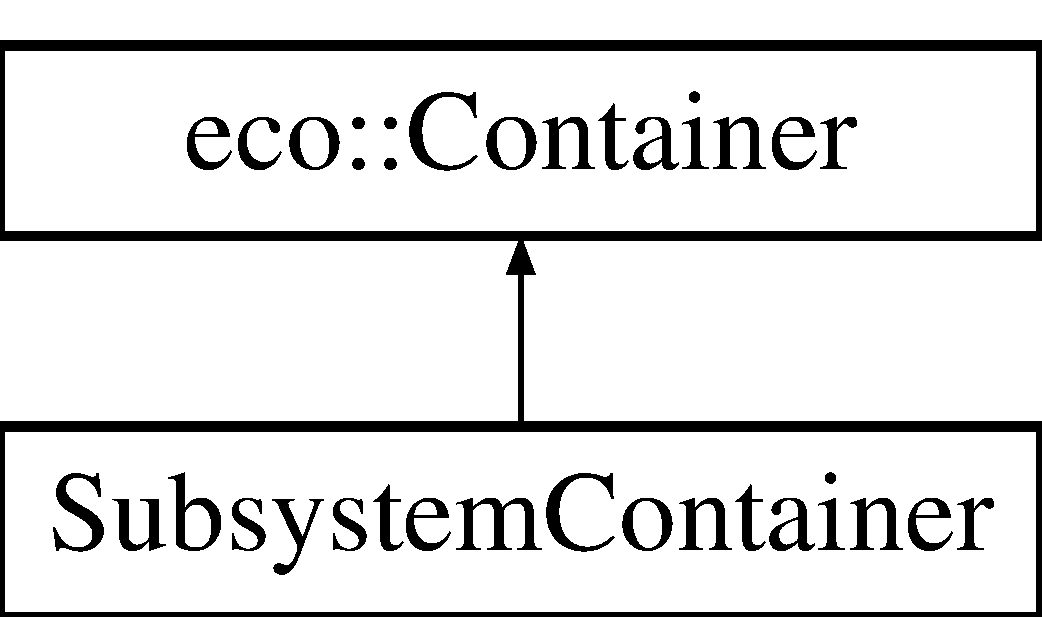
\includegraphics[height=2.000000cm]{classSubsystemContainer}
\end{center}
\end{figure}
\subsection*{Classes}
\begin{DoxyCompactItemize}
\item 
struct \hyperlink{structSubsystemContainer_1_1eat}{eat}
\begin{DoxyCompactList}\small\item\em boost multyindex::ordered\_\-index tag \end{DoxyCompactList}\item 
struct \hyperlink{structSubsystemContainer_1_1id}{id}
\begin{DoxyCompactList}\small\item\em boost multyindex::ordered\_\-index tag \end{DoxyCompactList}\item 
struct \hyperlink{structSubsystemContainer_1_1reproduction}{reproduction}
\begin{DoxyCompactList}\small\item\em boost multyindex::ordered\_\-index tag \end{DoxyCompactList}\item 
struct \hyperlink{structSubsystemContainer_1_1spec__id}{spec\_\-id}
\begin{DoxyCompactList}\small\item\em boost multyindex::ordered\_\-index tag \end{DoxyCompactList}\end{DoxyCompactItemize}
\subsection*{Public Types}
\begin{DoxyCompactItemize}
\item 
typedef multi\_\-index\_\-container$<$ \hyperlink{classIndividualAnimal}{IndividualAnimal}, indexed\_\-by$<$ ordered\_\-non\_\-unique$<$ tag$<$ \hyperlink{structSubsystemContainer_1_1eat}{eat} $>$, composite\_\-key$<$ \hyperlink{classIndividualAnimal}{IndividualAnimal}, const\_\-mem\_\-fun$<$ \hyperlink{classSpecied}{Specied}, unsigned int,\&IndividualAnimal::species\_\-id $>$, const\_\-mem\_\-fun$<$ \hyperlink{classVivent}{Vivent}, unsigned int,\&IndividualAnimal::hp $>$ $>$ $>$, ordered\_\-non\_\-unique$<$ tag$<$ \hyperlink{structSubsystemContainer_1_1reproduction}{reproduction} $>$, composite\_\-key$<$ \hyperlink{classIndividualAnimal}{IndividualAnimal}, const\_\-mem\_\-fun$<$ \hyperlink{classSpecied}{Specied}, unsigned int,\&IndividualAnimal::species\_\-id $>$, const\_\-mem\_\-fun$<$ \hyperlink{classVivent}{Vivent}, \hyperlink{classGender}{Gender},\&IndividualAnimal::gender $>$, const\_\-mem\_\-fun$<$ \hyperlink{classVivent}{Vivent}, unsigned int,\&IndividualAnimal::hp $>$ $>$ $>$, ordered\_\-unique$<$ tag$<$ \hyperlink{structSubsystemContainer_1_1id}{id} $>$, const\_\-mem\_\-fun$<$ \hyperlink{classExistance}{Existance}, \hyperlink{classExistance_a82c4092964457cd7da30d53072c62f1a}{Existance::id\_\-type},\&IndividualAnimal::id\_\-number $>$ $>$, ordered\_\-non\_\-unique$<$ tag$<$ \hyperlink{structSubsystemContainer_1_1spec__id}{spec\_\-id} $>$, const\_\-mem\_\-fun$<$ \hyperlink{classSpecied}{Specied}, unsigned int,\&IndividualAnimal::species\_\-id $>$ $>$ $>$$>$ \hyperlink{classSubsystemContainer_a8f87e58293188f19a139b1f9ac21fe3e}{animal\_\-set}
\begin{DoxyCompactList}\small\item\em animals container typedef \end{DoxyCompactList}\item 
\hypertarget{classSubsystemContainer_ad6392db27e78a340c21252e63edbe55f}{
typedef animal\_\-set::index$<$ \hyperlink{structSubsystemContainer_1_1eat}{eat} $>$::type \hyperlink{classSubsystemContainer_ad6392db27e78a340c21252e63edbe55f}{index\_\-an\_\-by\_\-eat}}
\label{classSubsystemContainer_ad6392db27e78a340c21252e63edbe55f}

\begin{DoxyCompactList}\small\item\em typedef for animal index 0 eat \end{DoxyCompactList}\item 
\hypertarget{classSubsystemContainer_a08f08e93dceda155601c8ff6ed31839e}{
typedef animal\_\-set::index$<$ \hyperlink{structSubsystemContainer_1_1reproduction}{reproduction} $>$::type \hyperlink{classSubsystemContainer_a08f08e93dceda155601c8ff6ed31839e}{index\_\-an\_\-by\_\-reproduce}}
\label{classSubsystemContainer_a08f08e93dceda155601c8ff6ed31839e}

\begin{DoxyCompactList}\small\item\em typedef for animal index 1 reproduce \end{DoxyCompactList}\item 
\hypertarget{classSubsystemContainer_ae095d19ad8aee4e1f1620166f440cf99}{
typedef animal\_\-set::index$<$ \hyperlink{structSubsystemContainer_1_1id}{id} $>$::type \hyperlink{classSubsystemContainer_ae095d19ad8aee4e1f1620166f440cf99}{index\_\-an\_\-by\_\-id}}
\label{classSubsystemContainer_ae095d19ad8aee4e1f1620166f440cf99}

\begin{DoxyCompactList}\small\item\em typedef for animal index 2 id\_\-number \end{DoxyCompactList}\item 
\hypertarget{classSubsystemContainer_a14b34b168bd55dd0b39a69795a65f4f8}{
typedef animal\_\-set::index$<$ \hyperlink{structSubsystemContainer_1_1spec__id}{spec\_\-id} $>$::type \hyperlink{classSubsystemContainer_a14b34b168bd55dd0b39a69795a65f4f8}{index\_\-an\_\-by\_\-spec\_\-id}}
\label{classSubsystemContainer_a14b34b168bd55dd0b39a69795a65f4f8}

\begin{DoxyCompactList}\small\item\em typedef for animal index 3 species\_\-id \end{DoxyCompactList}\item 
\hypertarget{classSubsystemContainer_a90723cf9f8cdae39e46ff65c5c898c2c}{
typedef index\_\-an\_\-by\_\-eat::iterator \hyperlink{classSubsystemContainer_a90723cf9f8cdae39e46ff65c5c898c2c}{an\_\-eat\_\-it}}
\label{classSubsystemContainer_a90723cf9f8cdae39e46ff65c5c898c2c}

\begin{DoxyCompactList}\small\item\em typedef for eat animal index iterator \end{DoxyCompactList}\item 
\hypertarget{classSubsystemContainer_a8ca51192ff066562729da7972e1c6d2e}{
typedef index\_\-an\_\-by\_\-eat::const\_\-iterator \hyperlink{classSubsystemContainer_a8ca51192ff066562729da7972e1c6d2e}{an\_\-eat\_\-const\_\-it}}
\label{classSubsystemContainer_a8ca51192ff066562729da7972e1c6d2e}

\begin{DoxyCompactList}\small\item\em typedef for eat animal index const iterator \end{DoxyCompactList}\item 
\hypertarget{classSubsystemContainer_aee4873426aef4e4f9f8d41ffb2b2f781}{
typedef index\_\-an\_\-by\_\-reproduce::iterator \hyperlink{classSubsystemContainer_aee4873426aef4e4f9f8d41ffb2b2f781}{an\_\-reproduce\_\-it}}
\label{classSubsystemContainer_aee4873426aef4e4f9f8d41ffb2b2f781}

\begin{DoxyCompactList}\small\item\em typedef for reproduce animal index iterator \end{DoxyCompactList}\item 
\hypertarget{classSubsystemContainer_ab227fa38862bc3645a12fa29b277c3c1}{
typedef index\_\-an\_\-by\_\-reproduce::const\_\-iterator \hyperlink{classSubsystemContainer_ab227fa38862bc3645a12fa29b277c3c1}{an\_\-reproduce\_\-const\_\-it}}
\label{classSubsystemContainer_ab227fa38862bc3645a12fa29b277c3c1}

\begin{DoxyCompactList}\small\item\em typedef for reproduce animal index const iterator \end{DoxyCompactList}\item 
\hypertarget{classSubsystemContainer_a016775688f9d4baed66e8bdc3fbc0ec9}{
typedef index\_\-an\_\-by\_\-id::iterator \hyperlink{classSubsystemContainer_a016775688f9d4baed66e8bdc3fbc0ec9}{an\_\-id\_\-it}}
\label{classSubsystemContainer_a016775688f9d4baed66e8bdc3fbc0ec9}

\begin{DoxyCompactList}\small\item\em typedef for id animal index iterator \end{DoxyCompactList}\item 
\hypertarget{classSubsystemContainer_a65c443ffed219d6e1d4c745bb98577e0}{
typedef index\_\-an\_\-by\_\-id::const\_\-iterator \hyperlink{classSubsystemContainer_a65c443ffed219d6e1d4c745bb98577e0}{an\_\-id\_\-const\_\-it}}
\label{classSubsystemContainer_a65c443ffed219d6e1d4c745bb98577e0}

\begin{DoxyCompactList}\small\item\em typedef for id animal index const iterator \end{DoxyCompactList}\item 
\hypertarget{classSubsystemContainer_a1126a7368a8724cd69ea707f6c90bd42}{
typedef index\_\-an\_\-by\_\-spec\_\-id::iterator \hyperlink{classSubsystemContainer_a1126a7368a8724cd69ea707f6c90bd42}{an\_\-spec\_\-id\_\-it}}
\label{classSubsystemContainer_a1126a7368a8724cd69ea707f6c90bd42}

\begin{DoxyCompactList}\small\item\em typedef for speces id animal index iterator \end{DoxyCompactList}\item 
\hypertarget{classSubsystemContainer_a7e66c6e5b6efcdaee148cbd72331ef34}{
typedef index\_\-an\_\-by\_\-spec\_\-id::const\_\-iterator \hyperlink{classSubsystemContainer_a7e66c6e5b6efcdaee148cbd72331ef34}{an\_\-spec\_\-id\_\-const\_\-it}}
\label{classSubsystemContainer_a7e66c6e5b6efcdaee148cbd72331ef34}

\begin{DoxyCompactList}\small\item\em typedef for speces id animal index const iterator \end{DoxyCompactList}\item 
typedef multi\_\-index\_\-container$<$ \hyperlink{classIndividualVegetable}{IndividualVegetable}, indexed\_\-by$<$ ordered\_\-non\_\-unique$<$ tag$<$ \hyperlink{structSubsystemContainer_1_1eat}{eat} $>$, composite\_\-key$<$ \hyperlink{classIndividualVegetable}{IndividualVegetable}, const\_\-mem\_\-fun$<$ \hyperlink{classSpecied}{Specied}, unsigned int,\&IndividualAnimal::species\_\-id $>$, const\_\-mem\_\-fun$<$ \hyperlink{classVivent}{Vivent}, unsigned int,\&IndividualAnimal::hp $>$ $>$ $>$, ordered\_\-unique$<$ tag$<$ \hyperlink{structSubsystemContainer_1_1id}{id} $>$, const\_\-mem\_\-fun$<$ \hyperlink{classExistance}{Existance}, \hyperlink{classExistance_a82c4092964457cd7da30d53072c62f1a}{Existance::id\_\-type},\&IndividualAnimal::id\_\-number $>$ $>$, ordered\_\-non\_\-unique$<$ tag$<$ \hyperlink{structSubsystemContainer_1_1spec__id}{spec\_\-id} $>$, const\_\-mem\_\-fun$<$ \hyperlink{classSpecied}{Specied}, unsigned int,\&IndividualAnimal::species\_\-id $>$ $>$ $>$$>$ \hyperlink{classSubsystemContainer_aa11de189765005941e3c055feceb3db0}{vegetable\_\-set}
\begin{DoxyCompactList}\small\item\em vegetables container typedef \end{DoxyCompactList}\item 
\hypertarget{classSubsystemContainer_a03a3aebd29f38555702dfe6414ca4042}{
typedef vegetable\_\-set::index$<$ \hyperlink{structSubsystemContainer_1_1eat}{eat} $>$::type \hyperlink{classSubsystemContainer_a03a3aebd29f38555702dfe6414ca4042}{index\_\-veg\_\-by\_\-eat}}
\label{classSubsystemContainer_a03a3aebd29f38555702dfe6414ca4042}

\begin{DoxyCompactList}\small\item\em typedef for vegetable index 0 eat \end{DoxyCompactList}\item 
\hypertarget{classSubsystemContainer_a9434fd23ddbbf223a7d839a4709f5eaf}{
typedef vegetable\_\-set::index$<$ \hyperlink{structSubsystemContainer_1_1id}{id} $>$::type \hyperlink{classSubsystemContainer_a9434fd23ddbbf223a7d839a4709f5eaf}{index\_\-veg\_\-by\_\-id}}
\label{classSubsystemContainer_a9434fd23ddbbf223a7d839a4709f5eaf}

\begin{DoxyCompactList}\small\item\em typedef for vegetable index 1 id\_\-number \end{DoxyCompactList}\item 
\hypertarget{classSubsystemContainer_afce6013ad63346c39bc0d0c68e0933e6}{
typedef vegetable\_\-set::index$<$ \hyperlink{structSubsystemContainer_1_1spec__id}{spec\_\-id} $>$::type \hyperlink{classSubsystemContainer_afce6013ad63346c39bc0d0c68e0933e6}{index\_\-veg\_\-by\_\-spec\_\-id}}
\label{classSubsystemContainer_afce6013ad63346c39bc0d0c68e0933e6}

\begin{DoxyCompactList}\small\item\em typedef for vegetable index 2 species\_\-id \end{DoxyCompactList}\item 
\hypertarget{classSubsystemContainer_a561754a392ebbecb9360bedd2256d587}{
typedef index\_\-veg\_\-by\_\-eat::iterator \hyperlink{classSubsystemContainer_a561754a392ebbecb9360bedd2256d587}{veg\_\-eat\_\-it}}
\label{classSubsystemContainer_a561754a392ebbecb9360bedd2256d587}

\begin{DoxyCompactList}\small\item\em typedef for eat vegetal index iterator \end{DoxyCompactList}\item 
\hypertarget{classSubsystemContainer_a62dc5939b59c39c3b4fa5227205526af}{
typedef index\_\-veg\_\-by\_\-eat::const\_\-iterator \hyperlink{classSubsystemContainer_a62dc5939b59c39c3b4fa5227205526af}{veg\_\-eat\_\-const\_\-it}}
\label{classSubsystemContainer_a62dc5939b59c39c3b4fa5227205526af}

\begin{DoxyCompactList}\small\item\em typedef for eat vegetal index const iterator \end{DoxyCompactList}\item 
\hypertarget{classSubsystemContainer_a646e7cb7968fdb78105d62bb685aca81}{
typedef index\_\-veg\_\-by\_\-id::iterator \hyperlink{classSubsystemContainer_a646e7cb7968fdb78105d62bb685aca81}{veg\_\-id\_\-it}}
\label{classSubsystemContainer_a646e7cb7968fdb78105d62bb685aca81}

\begin{DoxyCompactList}\small\item\em typedef for id vegetal index iterator \end{DoxyCompactList}\item 
\hypertarget{classSubsystemContainer_aeb7fcecc573d61fcc41cdef2dd9df838}{
typedef index\_\-veg\_\-by\_\-id::const\_\-iterator \hyperlink{classSubsystemContainer_aeb7fcecc573d61fcc41cdef2dd9df838}{veg\_\-id\_\-const\_\-it}}
\label{classSubsystemContainer_aeb7fcecc573d61fcc41cdef2dd9df838}

\begin{DoxyCompactList}\small\item\em typedef for id vegetal index const iterator \end{DoxyCompactList}\item 
\hypertarget{classSubsystemContainer_a142f6962467d951f6c4051661412c4a9}{
typedef index\_\-veg\_\-by\_\-spec\_\-id::iterator \hyperlink{classSubsystemContainer_a142f6962467d951f6c4051661412c4a9}{veg\_\-spec\_\-id\_\-it}}
\label{classSubsystemContainer_a142f6962467d951f6c4051661412c4a9}

\begin{DoxyCompactList}\small\item\em typedef for speces id vegetal index iterator \end{DoxyCompactList}\item 
\hypertarget{classSubsystemContainer_a70f2a2528b029427a691668cddc65754}{
typedef index\_\-veg\_\-by\_\-spec\_\-id::const\_\-iterator \hyperlink{classSubsystemContainer_a70f2a2528b029427a691668cddc65754}{veg\_\-spec\_\-id\_\-const\_\-it}}
\label{classSubsystemContainer_a70f2a2528b029427a691668cddc65754}

\begin{DoxyCompactList}\small\item\em typedef for speces id vegetal index const iterator \end{DoxyCompactList}\item 
typedef std::pair$<$ \hyperlink{classSubsystemContainer_a8f87e58293188f19a139b1f9ac21fe3e}{animal\_\-set}, \hyperlink{classSubsystemContainer_aa11de189765005941e3c055feceb3db0}{vegetable\_\-set} $>$ \hyperlink{classSubsystemContainer_a2c517c44fccdecc58869c24ab6d3f667}{subsystem\_\-tp}
\begin{DoxyCompactList}\small\item\em the type of the subsystem \end{DoxyCompactList}\end{DoxyCompactItemize}
\subsection*{Public Member Functions}
\begin{DoxyCompactItemize}
\item 
\hyperlink{classSubsystemContainer_ababfc3a959c6fab15c8613ad744e31d5}{SubsystemContainer} (unsigned int u\_\-x=0, unsigned int u\_\-y=0)
\begin{DoxyCompactList}\small\item\em default constructor \end{DoxyCompactList}\item 
\hypertarget{classSubsystemContainer_a96ff687276c5b911c83056367e4aa5d7}{
\hyperlink{classSubsystemContainer_a96ff687276c5b911c83056367e4aa5d7}{$\sim$SubsystemContainer} ()}
\label{classSubsystemContainer_a96ff687276c5b911c83056367e4aa5d7}

\begin{DoxyCompactList}\small\item\em default destructor \end{DoxyCompactList}\item 
virtual bool \hyperlink{classSubsystemContainer_abad57ab248735fded65abacb908a1b7c}{is\_\-full} ()
\begin{DoxyCompactList}\small\item\em is the container full \end{DoxyCompactList}\item 
virtual bool \hyperlink{classSubsystemContainer_ad3c757166da9538df858c550813124b0}{is\_\-full} (\hyperlink{classSpecied}{Specied} \&sample)
\begin{DoxyCompactList}\small\item\em is full for this species \end{DoxyCompactList}\item 
virtual bool \hyperlink{classSubsystemContainer_af1f07b97e8efbca22267479d68344783}{is\_\-full} (const unsigned int u\_\-spec\_\-id)
\begin{DoxyCompactList}\small\item\em is full for this species \end{DoxyCompactList}\item 
bool \hyperlink{classSubsystemContainer_a2d3ef6a5d11bc8744cdb3d98ba563056}{insert} (\hyperlink{classIndividualAnimal}{IndividualAnimal} \&an)
\begin{DoxyCompactList}\small\item\em insert a vivent \end{DoxyCompactList}\item 
\hypertarget{classSubsystemContainer_ae5575faff44dead9dada0cd8c95feef7}{
bool \hyperlink{classSubsystemContainer_ae5575faff44dead9dada0cd8c95feef7}{insert} (\hyperlink{classIndividualVegetable}{IndividualVegetable} \&veg)}
\label{classSubsystemContainer_ae5575faff44dead9dada0cd8c95feef7}

\begin{DoxyCompactList}\small\item\em insert a vivent \end{DoxyCompactList}\item 
bool \hyperlink{classSubsystemContainer_a4aebe195bf137309f42a528dd3771be0}{remove} (const long unsigned int u\_\-id)
\begin{DoxyCompactList}\small\item\em remove an animal \end{DoxyCompactList}\item 
\hyperlink{classSubsystemContainer_a016775688f9d4baed66e8bdc3fbc0ec9}{an\_\-id\_\-it} \hyperlink{classSubsystemContainer_a4d63b50ac6eefd3f322524fe99435574}{find\_\-animal} (const long unsigned int u\_\-id)
\begin{DoxyCompactList}\small\item\em find animal \end{DoxyCompactList}\item 
\hyperlink{classSubsystemContainer_a646e7cb7968fdb78105d62bb685aca81}{veg\_\-id\_\-it} \hyperlink{classSubsystemContainer_a403e286ac23c44b28e82acb3613d88c2}{find\_\-vegetable} (const long unsigned int u\_\-id)
\begin{DoxyCompactList}\small\item\em find vegetable \end{DoxyCompactList}\item 
std::pair$<$ unsigned int, bool $>$ \hyperlink{classSubsystemContainer_a383ac4ca92778f71ebc8d6610382b825}{count\_\-vivents} (const unsigned int u\_\-spec\_\-id=0, \hyperlink{classSpeciesController}{SpeciesController} u\_\-spec\_\-con=\hyperlink{classSpeciesController}{SpeciesController}(0))
\begin{DoxyCompactList}\small\item\em count the number of vivent in this subsystem \end{DoxyCompactList}\item 
std::pair$<$ unsigned int, bool $>$ \hyperlink{classSubsystemContainer_a4e9a8aabfe39a9a3abb283da0dc5acfa}{count\_\-vivents} (const \hyperlink{structSpeciesInfo}{SpeciesInfo} u\_\-spec\_\-info)
\begin{DoxyCompactList}\small\item\em count the number of vivent in this subsystem \end{DoxyCompactList}\item 
\hypertarget{classSubsystemContainer_a706f074071c227f63e6b7095fabee40f}{
\hyperlink{classSubsystemContainer_a2c517c44fccdecc58869c24ab6d3f667}{subsystem\_\-tp} \& \hyperlink{classSubsystemContainer_a706f074071c227f63e6b7095fabee40f}{sub\_\-ecosystem} ()}
\label{classSubsystemContainer_a706f074071c227f63e6b7095fabee40f}

\begin{DoxyCompactList}\small\item\em set the sub ecosystem \end{DoxyCompactList}\item 
\hypertarget{classSubsystemContainer_aaf2520b985e9173fafa07627fce7e832}{
\hyperlink{classSubsystemContainer_a8f87e58293188f19a139b1f9ac21fe3e}{animal\_\-set} \& \hyperlink{classSubsystemContainer_aaf2520b985e9173fafa07627fce7e832}{animal\_\-sub\_\-ecosystem} ()}
\label{classSubsystemContainer_aaf2520b985e9173fafa07627fce7e832}

\begin{DoxyCompactList}\small\item\em set animal\_\-set \end{DoxyCompactList}\item 
\hypertarget{classSubsystemContainer_a19515c2c6dd086d7d980216346ab2184}{
\hyperlink{classSubsystemContainer_aa11de189765005941e3c055feceb3db0}{vegetable\_\-set} \& \hyperlink{classSubsystemContainer_a19515c2c6dd086d7d980216346ab2184}{vegetable\_\-sub\_\-ecosystem} ()}
\label{classSubsystemContainer_a19515c2c6dd086d7d980216346ab2184}

\begin{DoxyCompactList}\small\item\em set vegetable\_\-set \end{DoxyCompactList}\item 
\hypertarget{classSubsystemContainer_ab3e74b7e84eaef44fe78ea9fba2da4a5}{
unsigned int \& \hyperlink{classSubsystemContainer_ab3e74b7e84eaef44fe78ea9fba2da4a5}{x\_\-position} ()}
\label{classSubsystemContainer_ab3e74b7e84eaef44fe78ea9fba2da4a5}

\begin{DoxyCompactList}\small\item\em set x\_\-position \end{DoxyCompactList}\item 
\hypertarget{classSubsystemContainer_a7b019b1b35557644630c5ff72de62243}{
unsigned int \& \hyperlink{classSubsystemContainer_a7b019b1b35557644630c5ff72de62243}{y\_\-position} ()}
\label{classSubsystemContainer_a7b019b1b35557644630c5ff72de62243}

\begin{DoxyCompactList}\small\item\em set y\_\-position \end{DoxyCompactList}\item 
\hypertarget{classSubsystemContainer_ae35bcf55318dd4be8d39ba60cf27ca31}{
const \hyperlink{classSubsystemContainer_a2c517c44fccdecc58869c24ab6d3f667}{subsystem\_\-tp} \& \hyperlink{classSubsystemContainer_ae35bcf55318dd4be8d39ba60cf27ca31}{sub\_\-ecosystem} () const }
\label{classSubsystemContainer_ae35bcf55318dd4be8d39ba60cf27ca31}

\begin{DoxyCompactList}\small\item\em get the sub ecosystem \end{DoxyCompactList}\item 
\hypertarget{classSubsystemContainer_aa5df163b7162b4250dfd9c115392a545}{
const \hyperlink{classSubsystemContainer_a8f87e58293188f19a139b1f9ac21fe3e}{animal\_\-set} \& \hyperlink{classSubsystemContainer_aa5df163b7162b4250dfd9c115392a545}{animal\_\-sub\_\-ecosystem} () const }
\label{classSubsystemContainer_aa5df163b7162b4250dfd9c115392a545}

\begin{DoxyCompactList}\small\item\em get animal\_\-set \end{DoxyCompactList}\item 
\hypertarget{classSubsystemContainer_a755d4d2106c2c474dea5a6b0065f15f7}{
const \hyperlink{classSubsystemContainer_aa11de189765005941e3c055feceb3db0}{vegetable\_\-set} \& \hyperlink{classSubsystemContainer_a755d4d2106c2c474dea5a6b0065f15f7}{vegetable\_\-sub\_\-ecosystem} () const }
\label{classSubsystemContainer_a755d4d2106c2c474dea5a6b0065f15f7}

\begin{DoxyCompactList}\small\item\em get vegetable\_\-set \end{DoxyCompactList}\item 
\hypertarget{classSubsystemContainer_a317b9541923b6c520e17b7f901131537}{
unsigned int \hyperlink{classSubsystemContainer_a317b9541923b6c520e17b7f901131537}{x\_\-position} () const }
\label{classSubsystemContainer_a317b9541923b6c520e17b7f901131537}

\begin{DoxyCompactList}\small\item\em get m\_\-x\_\-position \end{DoxyCompactList}\item 
\hypertarget{classSubsystemContainer_aa74c3e4ccf46c4c8941e86ffa07a6926}{
unsigned int \hyperlink{classSubsystemContainer_aa74c3e4ccf46c4c8941e86ffa07a6926}{y\_\-position} () const }
\label{classSubsystemContainer_aa74c3e4ccf46c4c8941e86ffa07a6926}

\begin{DoxyCompactList}\small\item\em get m\_\-y\_\-position \end{DoxyCompactList}\end{DoxyCompactItemize}
\subsection*{Private Attributes}
\begin{DoxyCompactItemize}
\item 
\hyperlink{classSubsystemContainer_a2c517c44fccdecc58869c24ab6d3f667}{subsystem\_\-tp} \hyperlink{classSubsystemContainer_aa85642dac44badafe0d6694c4e7893aa}{m\_\-sub\_\-ecosystem}
\begin{DoxyCompactList}\small\item\em the sub ecosistem \end{DoxyCompactList}\item 
\hypertarget{classSubsystemContainer_a2e69cbf8b4bb99b55020829c2036bcc8}{
unsigned int \hyperlink{classSubsystemContainer_a2e69cbf8b4bb99b55020829c2036bcc8}{m\_\-x\_\-position}}
\label{classSubsystemContainer_a2e69cbf8b4bb99b55020829c2036bcc8}

\begin{DoxyCompactList}\small\item\em x position of the subsystem in the ecosystem \end{DoxyCompactList}\item 
\hypertarget{classSubsystemContainer_afca7441a379efcea7d8b26a5ffa952a9}{
unsigned int \hyperlink{classSubsystemContainer_afca7441a379efcea7d8b26a5ffa952a9}{m\_\-y\_\-position}}
\label{classSubsystemContainer_afca7441a379efcea7d8b26a5ffa952a9}

\begin{DoxyCompactList}\small\item\em y position of the subsystem in the ecosystem \end{DoxyCompactList}\end{DoxyCompactItemize}
\subsection*{Friends}
\begin{DoxyCompactItemize}
\item 
std::ostream \& \hyperlink{classSubsystemContainer_acadf383984be65d380d82f1696afcd8a}{operator$<$$<$} (std::ostream \&os, const \hyperlink{classSubsystemContainer}{SubsystemContainer} \&subc)
\begin{DoxyCompactList}\small\item\em ostream operator of \hyperlink{classSubsystemContainer}{SubsystemContainer} \end{DoxyCompactList}\end{DoxyCompactItemize}


\subsection{Detailed Description}
sub ecosystem container 

this class contain the sub ecosistem composed by all individual animals and vegetables. 

Definition at line 69 of file subsystemcontainer.h.



\subsection{Member Typedef Documentation}
\hypertarget{classSubsystemContainer_a8f87e58293188f19a139b1f9ac21fe3e}{
\index{SubsystemContainer@{SubsystemContainer}!animal\_\-set@{animal\_\-set}}
\index{animal\_\-set@{animal\_\-set}!SubsystemContainer@{SubsystemContainer}}
\subsubsection[{animal\_\-set}]{\setlength{\rightskip}{0pt plus 5cm}typedef multi\_\-index\_\-container$<$ {\bf IndividualAnimal}, indexed\_\-by$<$ ordered\_\-non\_\-unique$<$ tag$<${\bf eat}$>$, composite\_\-key$<$ {\bf IndividualAnimal}, const\_\-mem\_\-fun$<$ {\bf Specied}, unsigned int, \&IndividualAnimal::species\_\-id $>$, const\_\-mem\_\-fun$<$ {\bf Vivent}, unsigned int, \&IndividualAnimal::hp $>$ $>$ $>$, ordered\_\-non\_\-unique$<$ tag$<${\bf reproduction}$>$, composite\_\-key$<$ {\bf IndividualAnimal}, const\_\-mem\_\-fun$<$ {\bf Specied}, unsigned int, \&IndividualAnimal::species\_\-id $>$, const\_\-mem\_\-fun$<$ {\bf Vivent}, {\bf Gender}, \&IndividualAnimal::gender $>$, const\_\-mem\_\-fun$<$ {\bf Vivent}, unsigned int, \&IndividualAnimal::hp $>$ $>$ $>$, ordered\_\-unique$<$ tag$<${\bf id}$>$, const\_\-mem\_\-fun$<$ {\bf Existance}, {\bf Existance::id\_\-type} , \&IndividualAnimal::id\_\-number $>$ $>$, ordered\_\-non\_\-unique$<$ tag$<${\bf spec\_\-id}$>$, const\_\-mem\_\-fun$<$ {\bf Specied}, unsigned int, \&IndividualAnimal::species\_\-id $>$ $>$ $>$$>$ {\bf SubsystemContainer::animal\_\-set}}}
\label{classSubsystemContainer_a8f87e58293188f19a139b1f9ac21fe3e}


animals container typedef 

following the boost::multi\_\-index tradition the typedef of this container is particularli cumbersome, but this is a small rate to pay in front of the extreme power of these containers

boost multi\_\-index containers gave us the possibility to sort and index the elements of a single container in different ways.

in addiction we uses the feature of composite\_\-key indexing. this give us the possibility (for example) to have contiguity for all the animals belonging to the same species and then have it sorted by ascendent hp.

in this implementation we have numerous indexes:


\begin{DoxyItemize}
\item 0 composite key index rappresenting the attitude to be eaten. \hyperlink{classIndividualAnimal}{IndividualAnimal} were sorted first by species\_\-id , then by hp.
\end{DoxyItemize}


\begin{DoxyItemize}
\item 1 composite key index rappresenting the \char`\"{}sexual charming\char`\"{} \hyperlink{classIndividualAnimal}{IndividualAnimal} were sorted first by species\_\-id , then by \hyperlink{classGender}{Gender} , and finally by hp;
\end{DoxyItemize}


\begin{DoxyItemize}
\item 2 order unique by the \hyperlink{classIndividualAnimal}{IndividualAnimal} id\_\-number. this means that no animals whith same id were admitted
\end{DoxyItemize}


\begin{DoxyItemize}
\item 3 order non unique by species id, this order is used to fast compute the number of animals of the same species and similar purposes 
\end{DoxyItemize}

Definition at line 189 of file subsystemcontainer.h.

\hypertarget{classSubsystemContainer_a2c517c44fccdecc58869c24ab6d3f667}{
\index{SubsystemContainer@{SubsystemContainer}!subsystem\_\-tp@{subsystem\_\-tp}}
\index{subsystem\_\-tp@{subsystem\_\-tp}!SubsystemContainer@{SubsystemContainer}}
\subsubsection[{subsystem\_\-tp}]{\setlength{\rightskip}{0pt plus 5cm}typedef std::pair$<${\bf animal\_\-set} , {\bf vegetable\_\-set}$>$ {\bf SubsystemContainer::subsystem\_\-tp}}}
\label{classSubsystemContainer_a2c517c44fccdecc58869c24ab6d3f667}


the type of the subsystem 

first member is an animal\_\-set second is a vegetable\_\-set 

Definition at line 334 of file subsystemcontainer.h.

\hypertarget{classSubsystemContainer_aa11de189765005941e3c055feceb3db0}{
\index{SubsystemContainer@{SubsystemContainer}!vegetable\_\-set@{vegetable\_\-set}}
\index{vegetable\_\-set@{vegetable\_\-set}!SubsystemContainer@{SubsystemContainer}}
\subsubsection[{vegetable\_\-set}]{\setlength{\rightskip}{0pt plus 5cm}typedef multi\_\-index\_\-container$<$ {\bf IndividualVegetable}, indexed\_\-by$<$ ordered\_\-non\_\-unique$<$ tag$<${\bf eat}$>$, composite\_\-key$<$ {\bf IndividualVegetable}, const\_\-mem\_\-fun$<$ {\bf Specied}, unsigned int, \&IndividualAnimal::species\_\-id $>$, const\_\-mem\_\-fun$<$ {\bf Vivent}, unsigned int, \&IndividualAnimal::hp $>$ $>$ $>$, ordered\_\-unique$<$ tag$<${\bf id}$>$, const\_\-mem\_\-fun$<$ {\bf Existance}, {\bf Existance::id\_\-type} , \&IndividualAnimal::id\_\-number $>$ $>$, ordered\_\-non\_\-unique$<$ tag$<${\bf spec\_\-id}$>$, const\_\-mem\_\-fun$<$ {\bf Specied}, unsigned int, \&IndividualAnimal::species\_\-id $>$ $>$ $>$$>$ {\bf SubsystemContainer::vegetable\_\-set}}}
\label{classSubsystemContainer_aa11de189765005941e3c055feceb3db0}


vegetables container typedef 

this container is similar but less complicated than the former. this is due to the fact that this version of the project does not implement vegetable reproduction.

\hyperlink{classVegetable}{Vegetable} can only be eaten so the indexes are:


\begin{DoxyItemize}
\item 0 composite key index rappresenting the attitude to be eaten. \hyperlink{classIndividualAnimal}{IndividualAnimal} were sorted first by species\_\-id , then by hp.
\end{DoxyItemize}


\begin{DoxyItemize}
\item 1 order unique by the \hyperlink{classIndividualAnimal}{IndividualAnimal} id\_\-number. this means that no animals whith same id were admitted
\end{DoxyItemize}


\begin{DoxyItemize}
\item 2 order non unique by species id, this order is used to fast compute the number of animals of the same species and similar purposes 
\end{DoxyItemize}

Definition at line 295 of file subsystemcontainer.h.



\subsection{Constructor \& Destructor Documentation}
\hypertarget{classSubsystemContainer_ababfc3a959c6fab15c8613ad744e31d5}{
\index{SubsystemContainer@{SubsystemContainer}!SubsystemContainer@{SubsystemContainer}}
\index{SubsystemContainer@{SubsystemContainer}!SubsystemContainer@{SubsystemContainer}}
\subsubsection[{SubsystemContainer}]{\setlength{\rightskip}{0pt plus 5cm}SubsystemContainer::SubsystemContainer (
\begin{DoxyParamCaption}
\item[{unsigned int}]{u\_\-x = {\ttfamily 0}, }
\item[{unsigned int}]{u\_\-y = {\ttfamily 0}}
\end{DoxyParamCaption}
)}}
\label{classSubsystemContainer_ababfc3a959c6fab15c8613ad744e31d5}


default constructor 

set's the position of the subsystem 
\begin{DoxyParams}{Parameters}
{\em u\_\-x} & x position \\
\hline
{\em u\_\-y} & y position \\
\hline
\end{DoxyParams}


Definition at line 39 of file subsystemcontainer.cpp.



\subsection{Member Function Documentation}
\hypertarget{classSubsystemContainer_a4e9a8aabfe39a9a3abb283da0dc5acfa}{
\index{SubsystemContainer@{SubsystemContainer}!count\_\-vivents@{count\_\-vivents}}
\index{count\_\-vivents@{count\_\-vivents}!SubsystemContainer@{SubsystemContainer}}
\subsubsection[{count\_\-vivents}]{\setlength{\rightskip}{0pt plus 5cm}std::pair$<$ unsigned int, bool $>$ SubC::count\_\-vivents (
\begin{DoxyParamCaption}
\item[{const {\bf SpeciesInfo}}]{u\_\-spec\_\-info}
\end{DoxyParamCaption}
)}}
\label{classSubsystemContainer_a4e9a8aabfe39a9a3abb283da0dc5acfa}


count the number of vivent in this subsystem 

returns the number of vivent of a determinate species id if no species id is indicated returns the total ammount of vivent 
\begin{DoxyParams}{Parameters}
{\em u\_\-spec\_\-info} & species info of the species \\
\hline
\end{DoxyParams}
\begin{DoxyReturn}{Returns}
a pair whit first member the number of vivent counted, at second member true if the info is correct, false if species info had noot been passed; 
\end{DoxyReturn}


Definition at line 426 of file subsystemcontainer.cpp.

\hypertarget{classSubsystemContainer_a383ac4ca92778f71ebc8d6610382b825}{
\index{SubsystemContainer@{SubsystemContainer}!count\_\-vivents@{count\_\-vivents}}
\index{count\_\-vivents@{count\_\-vivents}!SubsystemContainer@{SubsystemContainer}}
\subsubsection[{count\_\-vivents}]{\setlength{\rightskip}{0pt plus 5cm}std::pair$<$ unsigned int, bool $>$ SubC::count\_\-vivents (
\begin{DoxyParamCaption}
\item[{const unsigned int}]{u\_\-spec\_\-id = {\ttfamily 0}, }
\item[{{\bf SpeciesController}}]{u\_\-spec\_\-con = {\ttfamily {\bf SpeciesController}(0)}}
\end{DoxyParamCaption}
)}}
\label{classSubsystemContainer_a383ac4ca92778f71ebc8d6610382b825}


count the number of vivent in this subsystem 

returns the number of vivent of a determinate species id


\begin{DoxyParams}{Parameters}
{\em u\_\-spec\_\-id} & the species id of the species \\
\hline
{\em u\_\-spec\_\-con} & the species controller. necessary to determinate if vegetable or animal. \\
\hline
\end{DoxyParams}
\begin{DoxyReturn}{Returns}
a pair whit first member the number of vivent counted, at second member true if the spec id is correct, false if spec id is not correct or \hyperlink{classSpeciesController}{SpeciesController} had not been passed 
\end{DoxyReturn}


Definition at line 389 of file subsystemcontainer.cpp.

\hypertarget{classSubsystemContainer_a4d63b50ac6eefd3f322524fe99435574}{
\index{SubsystemContainer@{SubsystemContainer}!find\_\-animal@{find\_\-animal}}
\index{find\_\-animal@{find\_\-animal}!SubsystemContainer@{SubsystemContainer}}
\subsubsection[{find\_\-animal}]{\setlength{\rightskip}{0pt plus 5cm}{\bf SubC::an\_\-id\_\-it} SubC::find\_\-animal (
\begin{DoxyParamCaption}
\item[{const long unsigned int}]{u\_\-id}
\end{DoxyParamCaption}
)}}
\label{classSubsystemContainer_a4d63b50ac6eefd3f322524fe99435574}


find animal 

returns an iterator to the searched vivent 
\begin{DoxyParams}{Parameters}
{\em u\_\-id} & id of the animal to search to \\
\hline
\end{DoxyParams}
\begin{DoxyReturn}{Returns}
id iterator of the id index pointing to the searched animal. if not found returns end() 
\end{DoxyReturn}


Definition at line 358 of file subsystemcontainer.cpp.

\hypertarget{classSubsystemContainer_a403e286ac23c44b28e82acb3613d88c2}{
\index{SubsystemContainer@{SubsystemContainer}!find\_\-vegetable@{find\_\-vegetable}}
\index{find\_\-vegetable@{find\_\-vegetable}!SubsystemContainer@{SubsystemContainer}}
\subsubsection[{find\_\-vegetable}]{\setlength{\rightskip}{0pt plus 5cm}{\bf SubC::veg\_\-id\_\-it} SubC::find\_\-vegetable (
\begin{DoxyParamCaption}
\item[{const long unsigned int}]{u\_\-id}
\end{DoxyParamCaption}
)}}
\label{classSubsystemContainer_a403e286ac23c44b28e82acb3613d88c2}


find vegetable 

returns an iterator to the searched vivent 
\begin{DoxyParams}{Parameters}
{\em u\_\-id} & id of the vegetable to search to \\
\hline
\end{DoxyParams}
\begin{DoxyReturn}{Returns}
id iterator of the id index pointing to the searched vegetable. if not found returns end() 
\end{DoxyReturn}


Definition at line 372 of file subsystemcontainer.cpp.

\hypertarget{classSubsystemContainer_a2d3ef6a5d11bc8744cdb3d98ba563056}{
\index{SubsystemContainer@{SubsystemContainer}!insert@{insert}}
\index{insert@{insert}!SubsystemContainer@{SubsystemContainer}}
\subsubsection[{insert}]{\setlength{\rightskip}{0pt plus 5cm}bool SubC::insert (
\begin{DoxyParamCaption}
\item[{{\bf IndividualAnimal} \&}]{an}
\end{DoxyParamCaption}
)}}
\label{classSubsystemContainer_a2d3ef6a5d11bc8744cdb3d98ba563056}


insert a vivent 

return true if the vivent had been inserted correctly 

Definition at line 284 of file subsystemcontainer.cpp.

\hypertarget{classSubsystemContainer_ad3c757166da9538df858c550813124b0}{
\index{SubsystemContainer@{SubsystemContainer}!is\_\-full@{is\_\-full}}
\index{is\_\-full@{is\_\-full}!SubsystemContainer@{SubsystemContainer}}
\subsubsection[{is\_\-full}]{\setlength{\rightskip}{0pt plus 5cm}bool SubC::is\_\-full (
\begin{DoxyParamCaption}
\item[{{\bf Specied} \&}]{sample}
\end{DoxyParamCaption}
)\hspace{0.3cm}{\ttfamily  \mbox{[}virtual\mbox{]}}}}
\label{classSubsystemContainer_ad3c757166da9538df858c550813124b0}


is full for this species 


\begin{DoxyParams}{Parameters}
{\em sample} & sample specied animal to control free space \\
\hline
\end{DoxyParams}


Definition at line 118 of file subsystemcontainer.cpp.

\hypertarget{classSubsystemContainer_abad57ab248735fded65abacb908a1b7c}{
\index{SubsystemContainer@{SubsystemContainer}!is\_\-full@{is\_\-full}}
\index{is\_\-full@{is\_\-full}!SubsystemContainer@{SubsystemContainer}}
\subsubsection[{is\_\-full}]{\setlength{\rightskip}{0pt plus 5cm}bool SubC::is\_\-full (
\begin{DoxyParamCaption}
{}
\end{DoxyParamCaption}
)\hspace{0.3cm}{\ttfamily  \mbox{[}virtual\mbox{]}}}}
\label{classSubsystemContainer_abad57ab248735fded65abacb908a1b7c}


is the container full 

potrebbe restare per implementazioni barbare del tipo: c'è ancora spazio per qualcosa? 

Implements \hyperlink{classeco_1_1Container_aaba4667933eb47147b319f6daa7da5c2}{eco::Container}.



Definition at line 278 of file subsystemcontainer.cpp.

\hypertarget{classSubsystemContainer_af1f07b97e8efbca22267479d68344783}{
\index{SubsystemContainer@{SubsystemContainer}!is\_\-full@{is\_\-full}}
\index{is\_\-full@{is\_\-full}!SubsystemContainer@{SubsystemContainer}}
\subsubsection[{is\_\-full}]{\setlength{\rightskip}{0pt plus 5cm}bool SubC::is\_\-full (
\begin{DoxyParamCaption}
\item[{const unsigned int}]{u\_\-spec\_\-id}
\end{DoxyParamCaption}
)\hspace{0.3cm}{\ttfamily  \mbox{[}virtual\mbox{]}}}}
\label{classSubsystemContainer_af1f07b97e8efbca22267479d68344783}


is full for this species 


\begin{DoxyParams}{Parameters}
{\em u\_\-spec\_\-id} & is the id of the species to controll \\
\hline
\end{DoxyParams}


Definition at line 125 of file subsystemcontainer.cpp.

\hypertarget{classSubsystemContainer_a4aebe195bf137309f42a528dd3771be0}{
\index{SubsystemContainer@{SubsystemContainer}!remove@{remove}}
\index{remove@{remove}!SubsystemContainer@{SubsystemContainer}}
\subsubsection[{remove}]{\setlength{\rightskip}{0pt plus 5cm}bool SubC::remove (
\begin{DoxyParamCaption}
\item[{const long unsigned int}]{u\_\-id}
\end{DoxyParamCaption}
)}}
\label{classSubsystemContainer_a4aebe195bf137309f42a528dd3771be0}


remove an animal 

remove the animal whith specified id return true if the operation succeed 
\begin{DoxyParams}{Parameters}
{\em u\_\-id} & id of the animal to be removed \\
\hline
\end{DoxyParams}


Definition at line 346 of file subsystemcontainer.cpp.



\subsection{Friends And Related Function Documentation}
\hypertarget{classSubsystemContainer_acadf383984be65d380d82f1696afcd8a}{
\index{SubsystemContainer@{SubsystemContainer}!operator$<$$<$@{operator$<$$<$}}
\index{operator$<$$<$@{operator$<$$<$}!SubsystemContainer@{SubsystemContainer}}
\subsubsection[{operator$<$$<$}]{\setlength{\rightskip}{0pt plus 5cm}std::ostream\& operator$<$$<$ (
\begin{DoxyParamCaption}
\item[{std::ostream \&}]{os, }
\item[{const {\bf SubsystemContainer} \&}]{subc}
\end{DoxyParamCaption}
)\hspace{0.3cm}{\ttfamily  \mbox{[}friend\mbox{]}}}}
\label{classSubsystemContainer_acadf383984be65d380d82f1696afcd8a}


ostream operator of \hyperlink{classSubsystemContainer}{SubsystemContainer} 

modify the stream printing:


\begin{DoxyItemize}
\item the susbsytem coordinates
\item animal\_\-set size
\item vegetable\_\-set size
\item all the animals and the vegetables 
\end{DoxyItemize}

\subsection{Member Data Documentation}
\hypertarget{classSubsystemContainer_aa85642dac44badafe0d6694c4e7893aa}{
\index{SubsystemContainer@{SubsystemContainer}!m\_\-sub\_\-ecosystem@{m\_\-sub\_\-ecosystem}}
\index{m\_\-sub\_\-ecosystem@{m\_\-sub\_\-ecosystem}!SubsystemContainer@{SubsystemContainer}}
\subsubsection[{m\_\-sub\_\-ecosystem}]{\setlength{\rightskip}{0pt plus 5cm}{\bf subsystem\_\-tp} {\bf SubsystemContainer::m\_\-sub\_\-ecosystem}\hspace{0.3cm}{\ttfamily  \mbox{[}private\mbox{]}}}}
\label{classSubsystemContainer_aa85642dac44badafe0d6694c4e7893aa}


the sub ecosistem 

contains animals and vegetables 

Definition at line 489 of file subsystemcontainer.h.



The documentation for this class was generated from the following files:\begin{DoxyCompactItemize}
\item 
sources/\hyperlink{subsystemcontainer_8h}{subsystemcontainer.h}\item 
sources/\hyperlink{subsystemcontainer_8cpp}{subsystemcontainer.cpp}\end{DoxyCompactItemize}

\hypertarget{classVegetable}{
\section{Vegetable Class Reference}
\label{classVegetable}\index{Vegetable@{Vegetable}}
}


class \hyperlink{classVegetable}{Vegetable}  




{\ttfamily \#include $<$vegetable.h$>$}

Inheritance diagram for Vegetable:\begin{figure}[H]
\begin{center}
\leavevmode
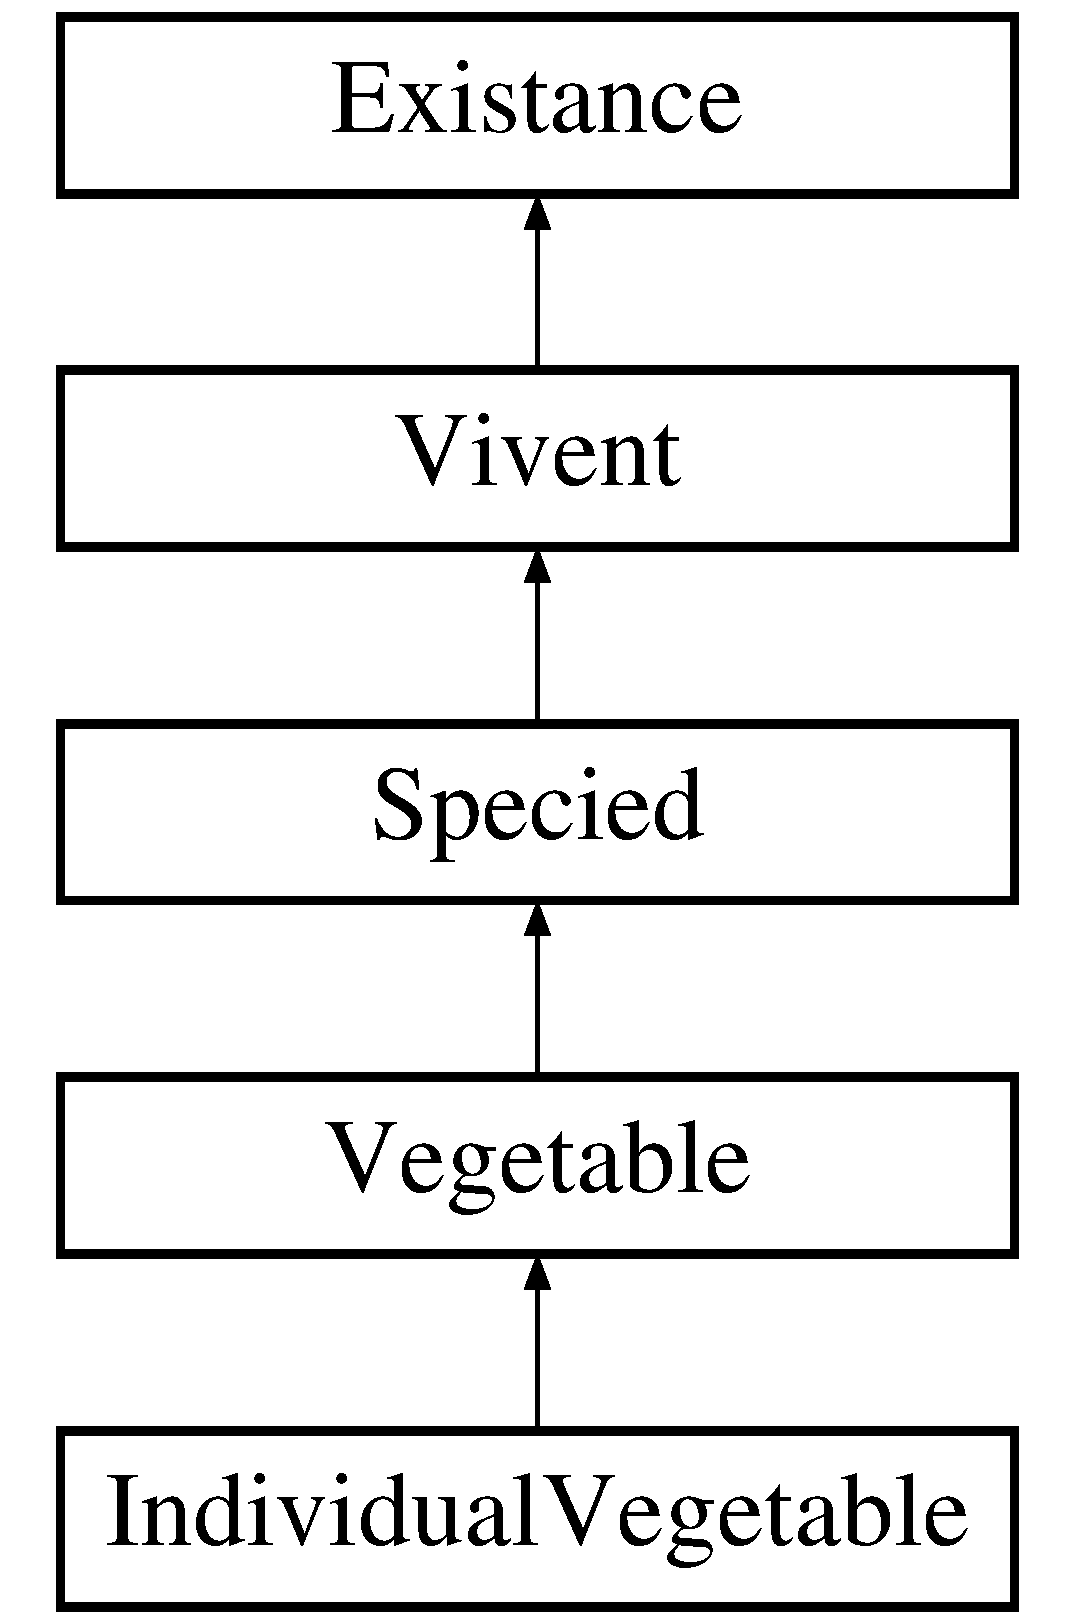
\includegraphics[height=5.000000cm]{classVegetable}
\end{center}
\end{figure}
\subsection*{Public Member Functions}
\begin{DoxyCompactItemize}
\item 
\hypertarget{classVegetable_a1f35f51f2f825b67f6db25ee3e228b47}{
\hyperlink{classVegetable_a1f35f51f2f825b67f6db25ee3e228b47}{Vegetable} ()}
\label{classVegetable_a1f35f51f2f825b67f6db25ee3e228b47}

\begin{DoxyCompactList}\small\item\em deafult constructor \end{DoxyCompactList}\item 
\hypertarget{classVegetable_a310e8097b46d2788d9da6adf08230180}{
\hyperlink{classVegetable_a310e8097b46d2788d9da6adf08230180}{$\sim$Vegetable} ()}
\label{classVegetable_a310e8097b46d2788d9da6adf08230180}

\begin{DoxyCompactList}\small\item\em default destructor \end{DoxyCompactList}\end{DoxyCompactItemize}


\subsection{Detailed Description}
class \hyperlink{classVegetable}{Vegetable} 

this class is present only for a modeling purpose. his implementation is given to future generations. 

Definition at line 36 of file vegetable.h.



The documentation for this class was generated from the following files:\begin{DoxyCompactItemize}
\item 
sources/\hyperlink{vegetable_8h}{vegetable.h}\item 
sources/\hyperlink{vegetable_8cpp}{vegetable.cpp}\end{DoxyCompactItemize}

\hypertarget{classVivent}{
\section{Vivent Class Reference}
\label{classVivent}\index{Vivent@{Vivent}}
}


class \hyperlink{classVivent}{Vivent} contain HP  




{\ttfamily \#include $<$vivent.h$>$}

Inheritance diagram for Vivent:\begin{figure}[H]
\begin{center}
\leavevmode
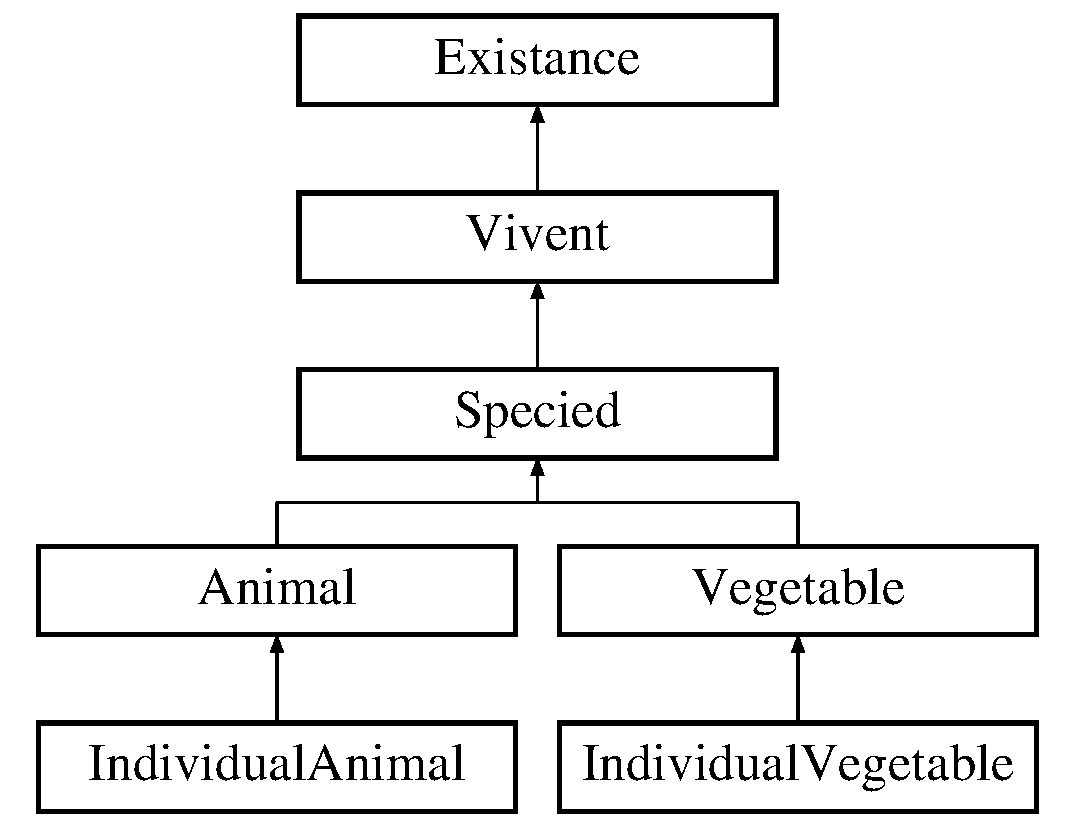
\includegraphics[height=5.000000cm]{classVivent}
\end{center}
\end{figure}
\subsection*{Public Member Functions}
\begin{DoxyCompactItemize}
\item 
\hyperlink{classVivent_a72647b9b0f4fe83f8f7360a6ed6e0ca7}{Vivent} (unsigned int u\_\-hp=100, \hyperlink{classGender}{Gender} u\_\-gender=\hyperlink{classGender}{Gender}(\char`\"{}asexual\char`\"{}))
\begin{DoxyCompactList}\small\item\em default constructor \end{DoxyCompactList}\item 
\hyperlink{classVivent_ac926725fd801a82fee9f960ff96386bf}{$\sim$Vivent} ()
\begin{DoxyCompactList}\small\item\em default destructor \end{DoxyCompactList}\item 
virtual bool \hyperlink{classVivent_a253291090ae6207f8f51f8ff669d9d17}{is\_\-alive} ()=0
\begin{DoxyCompactList}\small\item\em is\_\-alive \end{DoxyCompactList}\item 
unsigned int \& \hyperlink{classVivent_a5649888ad4779d5294fe7a6f57e4ecd4}{hp} ()
\begin{DoxyCompactList}\small\item\em the hp \end{DoxyCompactList}\item 
\hyperlink{classGender}{Gender} \& \hyperlink{classVivent_a83a8f9dd53a46f84ac01f3f262b7f6f4}{gender} ()
\begin{DoxyCompactList}\small\item\em the gender \end{DoxyCompactList}\item 
\hypertarget{classVivent_ad55d988e84cd95d0847a374a2102ee89}{
unsigned int \hyperlink{classVivent_ad55d988e84cd95d0847a374a2102ee89}{hp} () const }
\label{classVivent_ad55d988e84cd95d0847a374a2102ee89}

\begin{DoxyCompactList}\small\item\em get the hp \end{DoxyCompactList}\item 
\hypertarget{classVivent_a60975c27c18684b46e5fa2e1810c53ae}{
\hyperlink{classGender}{Gender} \hyperlink{classVivent_a60975c27c18684b46e5fa2e1810c53ae}{gender} () const }
\label{classVivent_a60975c27c18684b46e5fa2e1810c53ae}

\begin{DoxyCompactList}\small\item\em get the gender \end{DoxyCompactList}\end{DoxyCompactItemize}
\subsection*{Private Attributes}
\begin{DoxyCompactItemize}
\item 
unsigned int \hyperlink{classVivent_a6721d9dd0929a7bc729c67ab8528e8d9}{m\_\-hp}
\begin{DoxyCompactList}\small\item\em HP most important parameter. \end{DoxyCompactList}\item 
\hyperlink{classGender}{Gender} \hyperlink{classVivent_a0ea7b8eb35b129212059ad860015f695}{m\_\-gender}
\begin{DoxyCompactList}\small\item\em gender of the form of life \end{DoxyCompactList}\end{DoxyCompactItemize}


\subsection{Detailed Description}
class \hyperlink{classVivent}{Vivent} contain HP 

the form of life seen as an object able to live 

Definition at line 39 of file vivent.h.



\subsection{Constructor \& Destructor Documentation}
\hypertarget{classVivent_a72647b9b0f4fe83f8f7360a6ed6e0ca7}{
\index{Vivent@{Vivent}!Vivent@{Vivent}}
\index{Vivent@{Vivent}!Vivent@{Vivent}}
\subsubsection[{Vivent}]{\setlength{\rightskip}{0pt plus 5cm}Vivent::Vivent (
\begin{DoxyParamCaption}
\item[{unsigned int}]{u\_\-hp = {\ttfamily 100}, }
\item[{{\bf Gender}}]{u\_\-gender = {\ttfamily {\bf Gender}(\char`\"{}asexual\char`\"{})}}
\end{DoxyParamCaption}
)}}
\label{classVivent_a72647b9b0f4fe83f8f7360a6ed6e0ca7}


default constructor 

set's dm, default is hp = 100, gender asexual; 

Definition at line 34 of file vivent.cpp.

\hypertarget{classVivent_ac926725fd801a82fee9f960ff96386bf}{
\index{Vivent@{Vivent}!$\sim$Vivent@{$\sim$Vivent}}
\index{$\sim$Vivent@{$\sim$Vivent}!Vivent@{Vivent}}
\subsubsection[{$\sim$Vivent}]{\setlength{\rightskip}{0pt plus 5cm}Vivent::$\sim$Vivent (
\begin{DoxyParamCaption}
{}
\end{DoxyParamCaption}
)}}
\label{classVivent_ac926725fd801a82fee9f960ff96386bf}


default destructor 

does nothing 

Definition at line 41 of file vivent.cpp.



\subsection{Member Function Documentation}
\hypertarget{classVivent_a83a8f9dd53a46f84ac01f3f262b7f6f4}{
\index{Vivent@{Vivent}!gender@{gender}}
\index{gender@{gender}!Vivent@{Vivent}}
\subsubsection[{gender}]{\setlength{\rightskip}{0pt plus 5cm}{\bf Gender} \& Vivent::gender (
\begin{DoxyParamCaption}
{}
\end{DoxyParamCaption}
)}}
\label{classVivent_a83a8f9dd53a46f84ac01f3f262b7f6f4}


the gender 

\begin{DoxySeeAlso}{See also}
\hyperlink{classVivent_a0ea7b8eb35b129212059ad860015f695}{m\_\-gender} 
\end{DoxySeeAlso}


Definition at line 55 of file vivent.cpp.

\hypertarget{classVivent_a5649888ad4779d5294fe7a6f57e4ecd4}{
\index{Vivent@{Vivent}!hp@{hp}}
\index{hp@{hp}!Vivent@{Vivent}}
\subsubsection[{hp}]{\setlength{\rightskip}{0pt plus 5cm}unsigned int \& Vivent::hp (
\begin{DoxyParamCaption}
{}
\end{DoxyParamCaption}
)}}
\label{classVivent_a5649888ad4779d5294fe7a6f57e4ecd4}


the hp 

\begin{DoxySeeAlso}{See also}
\hyperlink{classVivent_a6721d9dd0929a7bc729c67ab8528e8d9}{m\_\-hp} 
\end{DoxySeeAlso}


Definition at line 45 of file vivent.cpp.

\hypertarget{classVivent_a253291090ae6207f8f51f8ff669d9d17}{
\index{Vivent@{Vivent}!is\_\-alive@{is\_\-alive}}
\index{is\_\-alive@{is\_\-alive}!Vivent@{Vivent}}
\subsubsection[{is\_\-alive}]{\setlength{\rightskip}{0pt plus 5cm}virtual bool Vivent::is\_\-alive (
\begin{DoxyParamCaption}
{}
\end{DoxyParamCaption}
)\hspace{0.3cm}{\ttfamily  \mbox{[}pure virtual\mbox{]}}}}
\label{classVivent_a253291090ae6207f8f51f8ff669d9d17}


is\_\-alive 

\begin{DoxySeeAlso}{See also}
\hyperlink{classExistance_ab86c25a779d30c45e26031e47c7b45dc}{Existance::is\_\-alive()} 
\end{DoxySeeAlso}


Implements \hyperlink{classExistance_ab86c25a779d30c45e26031e47c7b45dc}{Existance}.



Implemented in \hyperlink{classIndividualAnimal_a78960ddab5b3649638ba6b97238edc06}{IndividualAnimal}, and \hyperlink{classSpecied_a2173ab978d5cd2c2de4e25a4d6eb3152}{Specied}.



\subsection{Member Data Documentation}
\hypertarget{classVivent_a0ea7b8eb35b129212059ad860015f695}{
\index{Vivent@{Vivent}!m\_\-gender@{m\_\-gender}}
\index{m\_\-gender@{m\_\-gender}!Vivent@{Vivent}}
\subsubsection[{m\_\-gender}]{\setlength{\rightskip}{0pt plus 5cm}{\bf Gender} {\bf Vivent::m\_\-gender}\hspace{0.3cm}{\ttfamily  \mbox{[}private\mbox{]}}}}
\label{classVivent_a0ea7b8eb35b129212059ad860015f695}


gender of the form of life 

every form of life could be male, female, hermaphrodite (both) or asexual (nothing). it's not in our purpose to implement vegetable's gender and hermaphrodite. but, for correctnes and thinking to future realises, gender is included in this adstract class. gender is default setted to no asexual. 

Definition at line 91 of file vivent.h.

\hypertarget{classVivent_a6721d9dd0929a7bc729c67ab8528e8d9}{
\index{Vivent@{Vivent}!m\_\-hp@{m\_\-hp}}
\index{m\_\-hp@{m\_\-hp}!Vivent@{Vivent}}
\subsubsection[{m\_\-hp}]{\setlength{\rightskip}{0pt plus 5cm}unsigned int {\bf Vivent::m\_\-hp}\hspace{0.3cm}{\ttfamily  \mbox{[}private\mbox{]}}}}
\label{classVivent_a6721d9dd0929a7bc729c67ab8528e8d9}


HP most important parameter. 

it rappresents the health of the form of life whith a value of 0 the animal is dead whith a value of 100 the animal feels very good 

Definition at line 82 of file vivent.h.



The documentation for this class was generated from the following files:\begin{DoxyCompactItemize}
\item 
sources/\hyperlink{vivent_8h}{vivent.h}\item 
sources/vivent.cpp\end{DoxyCompactItemize}

\chapter{File Documentation}
\hypertarget{animal_8cpp}{
\section{sources/animal.cpp File Reference}
\label{animal_8cpp}\index{sources/animal.cpp@{sources/animal.cpp}}
}
{\ttfamily \#include \char`\"{}animal.h\char`\"{}}\par


\subsection{Detailed Description}
implementation of class \hyperlink{classAnimal}{Animal} 

Definition in file \hyperlink{animal_8cpp_source}{animal.cpp}.


\hypertarget{animal_8h}{
\section{sources/animal.h File Reference}
\label{animal_8h}\index{sources/animal.h@{sources/animal.h}}
}
{\ttfamily \#include \char`\"{}specied.h\char`\"{}}\par
\subsection*{Classes}
\begin{DoxyCompactItemize}
\item 
class \hyperlink{classAnimal}{Animal}
\begin{DoxyCompactList}\small\item\em class \hyperlink{classAnimal}{Animal} \end{DoxyCompactList}\end{DoxyCompactItemize}


\subsection{Detailed Description}
interface of class \hyperlink{classAnimal}{Animal} 

Definition in file \hyperlink{animal_8h_source}{animal.h}.


\hypertarget{beeings_8h}{
\section{sources/beeings.h File Reference}
\label{beeings_8h}\index{sources/beeings.h@{sources/beeings.h}}
}
{\ttfamily \#include \char`\"{}existance.h\char`\"{}}\par
{\ttfamily \#include \char`\"{}vivent.h\char`\"{}}\par
{\ttfamily \#include \char`\"{}specied.h\char`\"{}}\par
{\ttfamily \#include \char`\"{}animal.h\char`\"{}}\par
{\ttfamily \#include \char`\"{}individualanimal.h\char`\"{}}\par
{\ttfamily \#include \char`\"{}vegetable.h\char`\"{}}\par
{\ttfamily \#include \char`\"{}individualvegetable.h\char`\"{}}\par


\subsection{Detailed Description}
this file is a wrapper include for al the librarys concerning the form of lifes as:


\begin{DoxyItemize}
\item \hyperlink{classExistance}{Existance}
\item \hyperlink{classVivent}{Vivent}
\item \hyperlink{classSpecied}{Specied}
\item \hyperlink{classAnimal}{Animal}
\item \hyperlink{classVegetable}{Vegetable}
\item \hyperlink{classIndividualAnimal}{IndividualAnimal}
\item \hyperlink{classIndividualVegetable}{IndividualVegetable} 
\end{DoxyItemize}

Definition in file \hyperlink{beeings_8h_source}{beeings.h}.


\hypertarget{classcompares_8hpp}{
\section{sources/classcompares.hpp File Reference}
\label{classcompares_8hpp}\index{sources/classcompares.hpp@{sources/classcompares.hpp}}
}
\subsection*{Classes}
\begin{DoxyCompactItemize}
\item 
struct \hyperlink{structLikeRefCmp}{LikeRefCmp}
\begin{DoxyCompactList}\small\item\em used in SpeciesInfo.h \end{DoxyCompactList}\item 
struct \hyperlink{structLikeFactorCmp}{LikeFactorCmp}
\end{DoxyCompactItemize}


\subsection{Detailed Description}
file containing the functors used to compare classes 

Definition in file \hyperlink{classcompares_8hpp_source}{classcompares.hpp}.


\hypertarget{controller_8h}{
\section{sources/controller.h File Reference}
\label{controller_8h}\index{sources/controller.h@{sources/controller.h}}
}
\subsection*{Classes}
\begin{DoxyCompactItemize}
\item 
class \hyperlink{classController}{Controller}
\begin{DoxyCompactList}\small\item\em class that generally controll \end{DoxyCompactList}\end{DoxyCompactItemize}


\subsection{Detailed Description}
this file contains the container abstract class 

Definition in file \hyperlink{controller_8h_source}{controller.h}.


\hypertarget{ecosystem_8h}{
\section{sources/ecosystem.h File Reference}
\label{ecosystem_8h}\index{sources/ecosystem.h@{sources/ecosystem.h}}
}
{\ttfamily \#include $<$string$>$}\par
{\ttfamily \#include $<$iostream$>$}\par
{\ttfamily \#include \char`\"{}boost/multi\_\-array.hpp\char`\"{}}\par
{\ttfamily \#include $<$boost/random/mersenne\_\-twister.hpp$>$}\par
{\ttfamily \#include $<$boost/random/uniform\_\-int.hpp$>$}\par
{\ttfamily \#include $<$boost/random/variate\_\-generator.hpp$>$}\par
{\ttfamily \#include \char`\"{}container.h\char`\"{}}\par
{\ttfamily \#include \char`\"{}subsystemcontainer.h\char`\"{}}\par
{\ttfamily \#include \char`\"{}speciescontroller.h\char`\"{}}\par
{\ttfamily \#include \char`\"{}steplog.hpp\char`\"{}}\par
\subsection*{Classes}
\begin{DoxyCompactItemize}
\item 
class \hyperlink{classEcosystemContainer}{EcosystemContainer}
\begin{DoxyCompactList}\small\item\em contains all the form of life \end{DoxyCompactList}\end{DoxyCompactItemize}


\subsection{Detailed Description}
the ecosystem contains all the form of life. is divided in subecosystems. \begin{DoxySeeAlso}{See also}
subecosystem 
\end{DoxySeeAlso}


Definition in file \hyperlink{ecosystem_8h_source}{ecosystem.h}.


\hypertarget{existance_8cpp}{
\section{sources/existance.cpp File Reference}
\label{existance_8cpp}\index{sources/existance.cpp@{sources/existance.cpp}}
}
{\ttfamily \#include \char`\"{}existance.h\char`\"{}}\par


\subsection{Detailed Description}
implementation of the Abstract class \hyperlink{classExistance}{Existance} 

Definition in file \hyperlink{existance_8cpp_source}{existance.cpp}.


\hypertarget{existance_8h}{
\section{sources/existance.h File Reference}
\label{existance_8h}\index{sources/existance.h@{sources/existance.h}}
}
{\ttfamily \#include \char`\"{}time.h\char`\"{}}\par
\subsection*{Classes}
\begin{DoxyCompactItemize}
\item 
class \hyperlink{classExistance}{Existance}
\begin{DoxyCompactList}\small\item\em class \hyperlink{classExistance}{Existance} the most abstracted object \end{DoxyCompactList}\end{DoxyCompactItemize}


\subsection{Detailed Description}
interface of the Abstract class \hyperlink{classExistance}{Existance} 

Definition in file \hyperlink{existance_8h_source}{existance.h}.


\hypertarget{fieldchangers_8hpp}{
\section{sources/fieldchangers.hpp File Reference}
\label{fieldchangers_8hpp}\index{sources/fieldchangers.hpp@{sources/fieldchangers.hpp}}
}
{\ttfamily \#include \char`\"{}beeings.h\char`\"{}}\par
\subsection*{Classes}
\begin{DoxyCompactItemize}
\item 
struct \hyperlink{structchange__animal__hp}{change\_\-animal\_\-hp}
\begin{DoxyCompactList}\small\item\em functor to change \hyperlink{classIndividualAnimal}{IndividualAnimal} hp \end{DoxyCompactList}\item 
struct \hyperlink{structchange__animal__libido}{change\_\-animal\_\-libido}
\begin{DoxyCompactList}\small\item\em functor to cahnge \hyperlink{classIndividualAnimal}{IndividualAnimal} libido \end{DoxyCompactList}\item 
struct \hyperlink{structchange__animal__appetite}{change\_\-animal\_\-appetite}
\begin{DoxyCompactList}\small\item\em functor to change \hyperlink{classIndividualAnimal}{IndividualAnimal} appetite \end{DoxyCompactList}\end{DoxyCompactItemize}


\subsection{Detailed Description}
this file include numberous functors (or unary function) used to change fields of individual animals or individual vegetables (passed to the index::modify() member). 

Definition in file \hyperlink{fieldchangers_8hpp_source}{fieldchangers.hpp}.


\hypertarget{gender_8cpp}{
\section{sources/gender.cpp File Reference}
\label{gender_8cpp}\index{sources/gender.cpp@{sources/gender.cpp}}
}
{\ttfamily \#include $<$iostream$>$}\par
{\ttfamily \#include \char`\"{}gender.h\char`\"{}}\par
\subsection*{Functions}
\begin{DoxyCompactItemize}
\item 
std::ostream \& \hyperlink{gender_8cpp_a880decf4751cb0cf4d7b30cfa096a758}{operator$<$$<$} (std::ostream \&os, const \hyperlink{classGender}{Gender} \&gen)
\begin{DoxyCompactList}\small\item\em ostream operator of gender \end{DoxyCompactList}\end{DoxyCompactItemize}


\subsection{Detailed Description}
class \hyperlink{classGender}{Gender} implementation 

Definition in file \hyperlink{gender_8cpp_source}{gender.cpp}.



\subsection{Function Documentation}
\hypertarget{gender_8cpp_a880decf4751cb0cf4d7b30cfa096a758}{
\index{gender.cpp@{gender.cpp}!operator$<$$<$@{operator$<$$<$}}
\index{operator$<$$<$@{operator$<$$<$}!gender.cpp@{gender.cpp}}
\subsubsection[{operator$<$$<$}]{\setlength{\rightskip}{0pt plus 5cm}std::ostream\& operator$<$$<$ (
\begin{DoxyParamCaption}
\item[{std::ostream \&}]{os, }
\item[{const {\bf Gender} \&}]{gen}
\end{DoxyParamCaption}
)}}
\label{gender_8cpp_a880decf4751cb0cf4d7b30cfa096a758}


ostream operator of gender 

prints a string saying the actual gender is a wrapper of \hyperlink{classGender_a454a9f9b3605d4df6ad3125fbcb78dd2}{Gender::gender()} 

Definition at line 213 of file gender.cpp.


\hypertarget{gender_8h}{
\section{sources/gender.h File Reference}
\label{gender_8h}\index{sources/gender.h@{sources/gender.h}}
}


gender class interface  


{\ttfamily \#include $<$string$>$}\par
{\ttfamily \#include $<$iostream$>$}\par
\subsection*{Classes}
\begin{DoxyCompactItemize}
\item 
class \hyperlink{classGender}{Gender}
\begin{DoxyCompactList}\small\item\em the gender of the form of life \end{DoxyCompactList}\end{DoxyCompactItemize}


\subsection{Detailed Description}
gender class interface 

Definition in file \hyperlink{gender_8h_source}{gender.h}.


\hypertarget{individualanimal_8cpp}{
\section{sources/individualanimal.cpp File Reference}
\label{individualanimal_8cpp}\index{sources/individualanimal.cpp@{sources/individualanimal.cpp}}
}
{\ttfamily \#include $<$iostream$>$}\par
{\ttfamily \#include \char`\"{}individualanimal.h\char`\"{}}\par
\subsection*{Functions}
\begin{DoxyCompactItemize}
\item 
std::ostream \& \hyperlink{individualanimal_8cpp_abaf2e3cb53c5c0004f0fa218ab980965}{operator$<$$<$} (std::ostream \&os, const \hyperlink{classIndividualAnimal}{IndividualAnimal} \&an)
\end{DoxyCompactItemize}


\subsection{Detailed Description}
contains the implementation of \hyperlink{classIndividualAnimal}{IndividualAnimal} 

Definition in file \hyperlink{individualanimal_8cpp_source}{individualanimal.cpp}.



\subsection{Function Documentation}
\hypertarget{individualanimal_8cpp_abaf2e3cb53c5c0004f0fa218ab980965}{
\index{individualanimal.cpp@{individualanimal.cpp}!operator$<$$<$@{operator$<$$<$}}
\index{operator$<$$<$@{operator$<$$<$}!individualanimal.cpp@{individualanimal.cpp}}
\subsubsection[{operator$<$$<$}]{\setlength{\rightskip}{0pt plus 5cm}std::ostream\& operator$<$$<$ (
\begin{DoxyParamCaption}
\item[{std::ostream \&}]{os, }
\item[{const {\bf IndividualAnimal} \&}]{an}
\end{DoxyParamCaption}
)}}
\label{individualanimal_8cpp_abaf2e3cb53c5c0004f0fa218ab980965}
prints al main info of the animal 

Definition at line 76 of file individualanimal.cpp.


\hypertarget{individualanimal_8h}{
\section{sources/individualanimal.h File Reference}
\label{individualanimal_8h}\index{sources/individualanimal.h@{sources/individualanimal.h}}
}
{\ttfamily \#include \char`\"{}animal.h\char`\"{}}\par
\subsection*{Classes}
\begin{DoxyCompactItemize}
\item 
class \hyperlink{classIndividualAnimal}{IndividualAnimal}
\begin{DoxyCompactList}\small\item\em class \hyperlink{classIndividualAnimal}{IndividualAnimal} \end{DoxyCompactList}\end{DoxyCompactItemize}


\subsection{Detailed Description}
this file contains the interface of \hyperlink{classIndividualAnimal}{IndividualAnimal} 

Definition in file \hyperlink{individualanimal_8h_source}{individualanimal.h}.


\hypertarget{individualvegetable_8h}{
\section{sources/individualvegetable.h File Reference}
\label{individualvegetable_8h}\index{sources/individualvegetable.h@{sources/individualvegetable.h}}
}
{\ttfamily \#include \char`\"{}vegetable.h\char`\"{}}\par
\subsection*{Classes}
\begin{DoxyCompactItemize}
\item 
class \hyperlink{classIndividualVegetable}{IndividualVegetable}
\begin{DoxyCompactList}\small\item\em class \hyperlink{classIndividualVegetable}{IndividualVegetable} \end{DoxyCompactList}\end{DoxyCompactItemize}


\subsection{Detailed Description}
implementation of \hyperlink{classIndividualVegetable}{IndividualVegetable}

interface of \hyperlink{classIndividualVegetable}{IndividualVegetable} 

Definition in file \hyperlink{individualvegetable_8h_source}{individualvegetable.h}.


\hypertarget{miscellaneus_8h}{
\section{sources/miscellaneus.h File Reference}
\label{miscellaneus_8h}\index{sources/miscellaneus.h@{sources/miscellaneus.h}}
}


wrapper containing miscellaneus and varius classes  


{\ttfamily \#include \char`\"{}gender.h\char`\"{}}\par


\subsection{Detailed Description}
wrapper containing miscellaneus and varius classes 

Definition in file \hyperlink{miscellaneus_8h_source}{miscellaneus.h}.


\hypertarget{specied_8h}{
\section{sources/specied.h File Reference}
\label{specied_8h}\index{sources/specied.h@{sources/specied.h}}
}
{\ttfamily \#include \char`\"{}vivent.h\char`\"{}}\par
{\ttfamily \#include $<$string$>$}\par
\subsection*{Classes}
\begin{DoxyCompactItemize}
\item 
class \hyperlink{classSpecied}{Specied}
\begin{DoxyCompactList}\small\item\em class \hyperlink{classSpecied}{Specied} the form of life as species belonger \end{DoxyCompactList}\end{DoxyCompactItemize}


\subsection{Detailed Description}
implementation of \hyperlink{classSpecied}{Specied}

this file contains the interface of the class \hyperlink{classSpecied}{Specied}. this class is one of the most important. 

Definition in file \hyperlink{specied_8h_source}{specied.h}.


\hypertarget{speciescontroller_8h}{
\section{sources/speciescontroller.h File Reference}
\label{speciescontroller_8h}\index{sources/speciescontroller.h@{sources/speciescontroller.h}}
}
{\ttfamily \#include $<$map$>$}\par
{\ttfamily \#include $<$iostream$>$}\par
{\ttfamily \#include $<$fstream$>$}\par
{\ttfamily \#include $<$string$>$}\par
{\ttfamily \#include \char`\"{}controller.h\char`\"{}}\par
{\ttfamily \#include \char`\"{}speciesinfo.h\char`\"{}}\par
\subsection*{Classes}
\begin{DoxyCompactItemize}
\item 
class \hyperlink{classSpeciesController}{SpeciesController}
\begin{DoxyCompactList}\small\item\em contain info about the species in the ecosystem \end{DoxyCompactList}\end{DoxyCompactItemize}


\subsection{Detailed Description}
\hyperlink{classSpeciesController}{SpeciesController} interface 

Definition in file \hyperlink{speciescontroller_8h_source}{speciescontroller.h}.


\hypertarget{speciesinfo_8h}{
\section{sources/speciesinfo.h File Reference}
\label{speciesinfo_8h}\index{sources/speciesinfo.h@{sources/speciesinfo.h}}
}
{\ttfamily \#include $<$string$>$}\par
{\ttfamily \#include $<$map$>$}\par
{\ttfamily \#include $<$iostream$>$}\par
{\ttfamily \#include $<$set$>$}\par
{\ttfamily \#include \char`\"{}boost/lexical\_\-cast.hpp\char`\"{}}\par
{\ttfamily \#include \char`\"{}specied.h\char`\"{}}\par
{\ttfamily \#include \char`\"{}like.h\char`\"{}}\par
{\ttfamily \#include \char`\"{}container.h\char`\"{}}\par
{\ttfamily \#include \char`\"{}classcompares.hpp\char`\"{}}\par
\subsection*{Classes}
\begin{DoxyCompactItemize}
\item 
struct \hyperlink{structSpeciesInfo}{SpeciesInfo}
\begin{DoxyCompactList}\small\item\em species info containers \end{DoxyCompactList}\end{DoxyCompactItemize}


\subsection{Detailed Description}


Definition in file \hyperlink{speciesinfo_8h_source}{speciesinfo.h}.


\hypertarget{subsystemcontainer_8cpp}{
\section{sources/subsystemcontainer.cpp File Reference}
\label{subsystemcontainer_8cpp}\index{sources/subsystemcontainer.cpp@{sources/subsystemcontainer.cpp}}
}
{\ttfamily \#include $<$iostream$>$}\par
{\ttfamily \#include \char`\"{}subsystemcontainer.h\char`\"{}}\par
\subsection*{Typedefs}
\begin{DoxyCompactItemize}
\item 
typedef \hyperlink{classSubsystemContainer}{SubsystemContainer} \hyperlink{subsystemcontainer_8cpp_a0ddaa7e93a753780cfed339618bf5759}{SubC}
\end{DoxyCompactItemize}
\subsection*{Functions}
\begin{DoxyCompactItemize}
\item 
std::ostream \& \hyperlink{subsystemcontainer_8cpp_a5ce26005390fbcbeb4c11d36d4021337}{operator$<$$<$} (std::ostream \&os, const \hyperlink{classSubsystemContainer}{SubC} \&subc)
\begin{DoxyCompactList}\small\item\em ostream operator of \hyperlink{classSubsystemContainer}{SubsystemContainer} \end{DoxyCompactList}\end{DoxyCompactItemize}


\subsection{Detailed Description}


Definition in file \hyperlink{subsystemcontainer_8cpp_source}{subsystemcontainer.cpp}.



\subsection{Typedef Documentation}
\hypertarget{subsystemcontainer_8cpp_a0ddaa7e93a753780cfed339618bf5759}{
\index{subsystemcontainer.cpp@{subsystemcontainer.cpp}!SubC@{SubC}}
\index{SubC@{SubC}!subsystemcontainer.cpp@{subsystemcontainer.cpp}}
\subsubsection[{SubC}]{\setlength{\rightskip}{0pt plus 5cm}typedef {\bf SubsystemContainer} {\bf SubC}}}
\label{subsystemcontainer_8cpp_a0ddaa7e93a753780cfed339618bf5759}
implementaions of \hyperlink{subsystemcontainer_8h}{subsystemcontainer.h} 

Definition at line 35 of file subsystemcontainer.cpp.



\subsection{Function Documentation}
\hypertarget{subsystemcontainer_8cpp_a5ce26005390fbcbeb4c11d36d4021337}{
\index{subsystemcontainer.cpp@{subsystemcontainer.cpp}!operator$<$$<$@{operator$<$$<$}}
\index{operator$<$$<$@{operator$<$$<$}!subsystemcontainer.cpp@{subsystemcontainer.cpp}}
\subsubsection[{operator$<$$<$}]{\setlength{\rightskip}{0pt plus 5cm}std::ostream\& operator$<$$<$ (
\begin{DoxyParamCaption}
\item[{std::ostream \&}]{os, }
\item[{const {\bf SubC} \&}]{subc}
\end{DoxyParamCaption}
)}}
\label{subsystemcontainer_8cpp_a5ce26005390fbcbeb4c11d36d4021337}


ostream operator of \hyperlink{classSubsystemContainer}{SubsystemContainer} 

modify the stream printing:


\begin{DoxyItemize}
\item the susbsytem coordinates
\item animal\_\-set size
\item vegetable\_\-set size
\item all the animals and the vegetables 
\end{DoxyItemize}

Definition at line 488 of file subsystemcontainer.cpp.


\hypertarget{subsystemcontainer_8h}{
\section{sources/subsystemcontainer.h File Reference}
\label{subsystemcontainer_8h}\index{sources/subsystemcontainer.h@{sources/subsystemcontainer.h}}
}
{\ttfamily \#include $<$utility$>$}\par
{\ttfamily \#include $<$boost/multi\_\-index\_\-container.hpp$>$}\par
{\ttfamily \#include $<$boost/multi\_\-index/ordered\_\-index.hpp$>$}\par
{\ttfamily \#include $<$boost/multi\_\-index/identity.hpp$>$}\par
{\ttfamily \#include $<$boost/multi\_\-index/member.hpp$>$}\par
{\ttfamily \#include $<$boost/multi\_\-index/mem\_\-fun.hpp$>$}\par
{\ttfamily \#include $<$boost/multi\_\-index/composite\_\-key.hpp$>$}\par
{\ttfamily \#include \char`\"{}container.h\char`\"{}}\par
{\ttfamily \#include \char`\"{}beeings.h\char`\"{}}\par
{\ttfamily \#include \char`\"{}speciescontroller.h\char`\"{}}\par
{\ttfamily \#include \char`\"{}speciesinfo.h\char`\"{}}\par
\subsection*{Classes}
\begin{DoxyCompactItemize}
\item 
class \hyperlink{classSubsystemContainer}{SubsystemContainer}
\begin{DoxyCompactList}\small\item\em sub ecosystem container \end{DoxyCompactList}\item 
struct \hyperlink{structSubsystemContainer_1_1id}{SubsystemContainer::id}
\begin{DoxyCompactList}\small\item\em boost multyindex::ordered\_\-index tag \end{DoxyCompactList}\item 
struct \hyperlink{structSubsystemContainer_1_1eat}{SubsystemContainer::eat}
\begin{DoxyCompactList}\small\item\em boost multyindex::ordered\_\-index tag \end{DoxyCompactList}\item 
struct \hyperlink{structSubsystemContainer_1_1reproduction}{SubsystemContainer::reproduction}
\begin{DoxyCompactList}\small\item\em boost multyindex::ordered\_\-index tag \end{DoxyCompactList}\item 
struct \hyperlink{structSubsystemContainer_1_1spec__id}{SubsystemContainer::spec\_\-id}
\begin{DoxyCompactList}\small\item\em boost multyindex::ordered\_\-index tag \end{DoxyCompactList}\end{DoxyCompactItemize}


\subsection{Detailed Description}
file of the subsystem container, it contains the specification of the container. 

Definition in file \hyperlink{subsystemcontainer_8h_source}{subsystemcontainer.h}.


\hypertarget{time_8h}{
\section{sources/time.h File Reference}
\label{time_8h}\index{sources/time.h@{sources/time.h}}
}


classes to manipulate and determine the time of the system  


{\ttfamily \#include $<$iostream$>$}\par
\subsection*{Classes}
\begin{DoxyCompactItemize}
\item 
class \hyperlink{classAbstractClock}{AbstractClock}
\begin{DoxyCompactList}\small\item\em abstract class for the clock \end{DoxyCompactList}\item 
class \hyperlink{classClock}{Clock}
\begin{DoxyCompactList}\small\item\em real clock able to give the time of the sistem \end{DoxyCompactList}\item 
class \hyperlink{classDateOfBirth}{DateOfBirth}
\begin{DoxyCompactList}\small\item\em simple class for the date of birh \end{DoxyCompactList}\end{DoxyCompactItemize}


\subsection{Detailed Description}
classes to manipulate and determine the time of the system is really difficult to determine time in this context.

we have developed two types of time: relative and absolute

relative time: the easyest way is to think to what is a ecosistem cicle. An ecosistem cicle is concluded when all the animals in the ecosistem where called. for \char`\"{}call\char`\"{} we intend every time a form of life interact with another form of life, so if an animal fight whith another this constitutes o total of 2 calls) as you can imagine it could be really difficult to controll that all the animals were called so if we give to te ecosistem cicle a value of 1, each call to an animal has the time value interval of 1/total\_\-number\_\-of\_\-forms\_\-of\_\-life present in the ecosistem. so the running relative time is the number of cicles passed and the quantiti of the cicle running

absolute time: nothing different from the number of calls occured from the creation of the first form of life 

Definition in file \hyperlink{time_8h_source}{time.h}.


\hypertarget{vegetable_8cpp}{
\section{sources/vegetable.cpp File Reference}
\label{vegetable_8cpp}\index{sources/vegetable.cpp@{sources/vegetable.cpp}}
}
{\ttfamily \#include \char`\"{}vegetable.h\char`\"{}}\par


\subsection{Detailed Description}
implementation of class \hyperlink{classVegetable}{Vegetable} 

Definition in file \hyperlink{vegetable_8cpp_source}{vegetable.cpp}.


\hypertarget{vegetable_8h}{
\section{sources/vegetable.h File Reference}
\label{vegetable_8h}\index{sources/vegetable.h@{sources/vegetable.h}}
}
{\ttfamily \#include \char`\"{}specied.h\char`\"{}}\par
\subsection*{Classes}
\begin{DoxyCompactItemize}
\item 
class \hyperlink{classVegetable}{Vegetable}
\begin{DoxyCompactList}\small\item\em class \hyperlink{classVegetable}{Vegetable} \end{DoxyCompactList}\end{DoxyCompactItemize}


\subsection{Detailed Description}
interface of class \hyperlink{classVegetable}{Vegetable} 

Definition in file \hyperlink{vegetable_8h_source}{vegetable.h}.


\hypertarget{vivent_8h}{
\section{sources/vivent.h File Reference}
\label{vivent_8h}\index{sources/vivent.h@{sources/vivent.h}}
}
{\ttfamily \#include \char`\"{}existance.h\char`\"{}}\par
{\ttfamily \#include \char`\"{}miscellaneus.h\char`\"{}}\par
\subsection*{Classes}
\begin{DoxyCompactItemize}
\item 
class \hyperlink{classVivent}{Vivent}
\begin{DoxyCompactList}\small\item\em class \hyperlink{classVivent}{Vivent} contain HP \end{DoxyCompactList}\end{DoxyCompactItemize}


\subsection{Detailed Description}
this file contains the implementation of \hyperlink{classVivent}{Vivent}

this file contains the interface of \hyperlink{classVivent}{Vivent} abstract class 

Definition in file \hyperlink{vivent_8h_source}{vivent.h}.


\printindex
\end{document}
